\documentclass[11pt]{article}
\usepackage{amsmath} %for formula formatting
\usepackage{amssymb}
\usepackage{mathtools}
\usepackage{fullpage}
\usepackage{bbm} % this lets us have a blackboard 1
\usepackage[T1]{fontenc} % improved font encoding
\usepackage[utf8]{inputenc} % for better handling of non-ASCII characters
\usepackage{lmodern} % font choice
\usepackage{algorithm}
%\usepackage{fontspec}
\usepackage{multirow}
%\usepackage{epigraph}
\usepackage{setspace}
\usepackage{booktabs}
\usepackage{esvect}
\usepackage{caption}
\usepackage{subcaption}
\usepackage{blkarray}

% BibLaTeX
\usepackage[
backend=bibtex,
%sorting=none,
sorting=nyvt,
bibstyle=ieee,
%bibstyle=plainnat,
citestyle=authoryear,
natbib=true,
url=false,
isbn=false,
doi=false,
eprint=false,
date=year,
uniquename=init,
]{biblatex}  %reference manager

\bibliography{HPT}
\DeclareBibliographyCategory{nondiss}


% prevent certain fields in references from printing in bibliography
\AtEveryBibitem{\clearfield{issn}}
\AtEveryBibitem{\clearlist{issn}}

\AtEveryBibitem{\clearfield{language}}
\AtEveryBibitem{\clearlist{language}}

\AtEveryBibitem{\clearfield{doi}}
\AtEveryBibitem{\clearlist{doi}}

\AtEveryBibitem{\clearfield{url}}
\AtEveryBibitem{\clearlist{url}}

\AtEveryBibitem{%
	\ifentrytype{online}
	{}
	{\clearfield{urlyear}\clearfield{urlmonth}\clearfield{urlday}}}

% JJ 2021-11-24:
\AtEveryBibitem{
	\clearfield{note}
	\clearfield{pagetotal}
	\clearfield{series}
	\clearlist{language}
}
\DeclareFieldFormat{pages}{#1}
\renewbibmacro{in:}{}
% This removes the comma in the citation style, so we get "Roberts 2016" instead of "Roberts, 2016"
% https://tex.stackexchange.com/questions/134063/how-to-add-a-comma-between-author-and-year
\renewcommand*{\nameyeardelim}{\space}

% TiKZ
\usepackage{tikz}
\usetikzlibrary{calc,intersections,through,backgrounds}
\usetikzlibrary{bayesnet}
\usepackage{tikzscale}
\usepackage{tkz-euclide}
\usepackage{tcolorbox}
\tcbuselibrary{skins,breakable}

% pgfplots
\usepackage{pgfplots}
\pgfplotsset{compat=1.8}

% Appendix
%\usepackage{appendix}

\usepackage{svg}
\DeclareUnicodeCharacter{2212}{-}
\usepackage{xltabular}
\usepackage{hyperref}


%%%%% Custom commands for Marx chapter -JJ 2022-01-21
% \BERT
\newcommand{\BERT}[0]{\texttt{BERT}}
% \comment: For removing big chunks with one command
%\newcommand{\comment}[1]{}
% de: For typesetting German words in parentheses after English words
\newcommand{\de}[1]{\textit{#1}}
% \dett: fixed-width German words
\newcommand{\dett}[1]{\texttt{#1}}
% \jj: For [visible in the pdf] notes to self
\newcommand{\jj}[1]{***[\textbf{#1}]***}

%%% Custom commands for math stuff
\newcommand{\cTFIDF}[0]{\textsf{cTFIDF}}
\newcommand{\prevec}[2]{\mathbf{pre}_{#1}^{#2}}
\newcommand{\postvec}[2]{\mathbf{post}_{#1}^{#2}}
\newcommand{\Lead}[2]{\mathsf{Lead}_{#1 \rightarrow #2}}
\newcommand{\Sim}[0]{\mathsf{sim}}
\newcommand{\Dist}[0]{\mathsf{dist}}
\newcommand{\CDist}[0]{\mathsf{dist}_\angle{}}
\newcommand{\EDist}[0]{\mathsf{dist}_{\ell^2}}
% For general word vectors
\newcommand{\wvec}[1]{\vv{\texttt{#1}}}
% For author-specific word vectors
\newcommand{\awvec}[2]{\vv{\texttt{#1}}_{#2}}
% For entities in text
\newcommand{\entity}[1]{\texttt{#1}}
% For entities in pgfplots
\newcommand{\entpgf}[1]{\texttt{#1}}
% For entity *vectors* in text
\newcommand{\entvec}[1]{\texttt{#1}}
% For relational vectors in text
\newcommand{\relvec}[1]{\textsf{#1}}
% For entity vectors in pgfplots
\newcommand{\entvecpgf}[1]{\vv{\texttt{#1}}}
% For relational vectors in images
\newcommand{\relvecpgf}[1]{\vv{\textsf{#1}}}

\newcommand*\rot{\rotatebox{90}}

\title{Meaning, Understanding, and Quantification in the History of Ideas}
\author{Jeff Jacobs\\\texttt{jjacobs3@cs.stanford.edu}}

\begin{document}
	
	\maketitle
	
\begin{abstract}
\noindent What are political thinkers \textit{doing} with their words when they write a text, engage in a debate, or give a speech? We propose a ``computational political theory'', pairing recent breakthroughs in computational linguistics with the hermeneutic practices of intellectual history, as a set of tools for mapping out the political-discursive fields within which ideas circulate. We show, via a series of historical case studies, how a particular class of computational-linguistic algorithms called word embeddings are able to capture subtle differences in how authors employ certain contested terms (liberty, freedom, sovereignty, etc.) by explicitly modeling both the words and the contexts they're used in across a corpus of texts. We argue that these context-sensitive language models thus represent powerful and underutilized tools for historical research, and provide a framework for their use in developing, testing, and revising our understandings of key questions in the history of political thought.
\end{abstract}

\doublespacing

%\singlespacing
%\epigraph{Even the most abstract works of political theory are never above the battle; they are always part of the battle itself.}{Quentin Skinner, \textit{Hobbes and Republican Liberty} \cite{skinner_hobbes_2008}, p. xv}
%
%\epigraph{The weapon of criticism cannot, of course, replace criticism by weapons. Material force must be overthrown by material force. But philosophy also becomes a material force, once it has gripped the masses.}{Karl Marx, ``Contribution to the Critique of Hegel's Philosophy of Right'', \textit{MECW V3, p. 182}}
%
%\epigraph{\textit{Worte sind auch Taten.}
%	
%	(Words are also deeds.)}{Wittgenstein,
%	%\textit{Philosophische Untersuchungen}
%	\textit{Philosophical Investigations} \cite{wittgenstein_philosophical_1953}, p. 155}
%\doublespacing
	
%\section{Abstract\label{sov:abstract}}

\tableofcontents

\section{Introduction}\label{sec:intro}

What are political thinkers \textit{doing} with their words when they perform a political speech act---when they publish a treatise, give a speech, argue for a piece of legislation, and so on? Since the 1960s a group of historians centered around Cambridge University professors Quentin Skinner, J. G. A. Pocock, and John Dunn have changed the way we understand several key political thinkers and texts,
%\footnote{The foundational works of these scholars (discussed below) focus primarily on thinkers of the 16th and 17th centuries: Machiavelli, Hobbes, and Locke in particular. As will become clear over the course of our argument, this focus on \textit{pre-industrial} political thinkers is not incidental; there are fundamental limitations to their approach which render studies of \textit{post}-17th-century thought---i.e., thought in the era of mass communication and literacy---infeasible without the aid of computational tools like those we introduce in the coming sections.}
by consciously developing and applying a linguistic-philosophical and \textit{context-sensitive} methodology which places this question at the center of historical inquiry \citep{skinner_meaning_1969, pocock_virtue_1985}. 
As part of this endeavor the Cambridge School, as this group came to be known, placed a strong emphasis on the need for historians to explicitly describe and justify the methodologies being employed in their studies\footnote{Pocock, in fact, puts the point more strongly, arguing that the Cambridge School \textit{introduced} this self-reflection into the field of intellectual history:
	\begin{quote}
		``it was only in the middle 1960s, with the first appearance of writings by Quentin Skinner, that historians of political thought began to state the logic of their own inquiry and pursue it into fields where it encountered the philosophy of language.'' \citep[p. 3]{pocock_virtue_1985}
	\end{quote}
	We explore this claim---placing the Cambridge School itself within its broader historical context to argue that Karl Popper, more so than Skinner, can be credited with introducing this focus (a focus whose lineage contains important political consequences)---in Section \ref{sec:methods-ling-cambridge} below.
}
Most Cambridge School works therefore begin with extensive methodological introductions, in which particular modes of inquiry are introduced and justified prior to their application in the remainder of the work. Kenneth Minogue describes Skinner's early work, for example, as
\begin{quote}
	``primarily of interest to philosophers not for its excellent account of European thought about the state but for the self-conscious philosophy which has gone into it. It is a rare historian who pauses to get his philosophy in order before he embarks on a major enterprise'' \citep[p. 176]{tully_meaning_1988}
\end{quote} %valid and invalid modes of inference \textit{ex ante}. 
Thus the first of the three volumes of Quentin Skinner's \textit{Visions of Politics}, for example, is entirely devoted to method (providing 209 pages of methodological justification before discussing the Renaissance and Thomas Hobbes in Volumes 2 and 3, respectively), while J. G. A. Pocock's \textit{Virtue, Commerce, and History} begins with an intensive 36-page treatise on methodology, applying lessons learned from prior investigations to refine his approach before embarking on the inquiries of the remainder of the book.

It was not their emphasis on method \textit{as such}, however, that set the Cambridge School apart from other historiographic schools---indeed, many other postwar hermeneutic approaches (e.g., Derridean deconstructivism) have also accumulated a vast methodological literature\footnote{See \cite{skinner_return_1990} or \cite{tully_meaning_1988}, for example, for conversations between Cambridge School practitioners and scholars representing a wide range of alternative hermeneutic perspectives.}. Rather, it was their focus on \textit{contextual analysis} of texts---their call to de-emphasize the ``so-called `classic texts'{} [...] and focus instead on the more general social and intellectual matrix out of which [these] works arose'' \citep[p. x]{skinner_foundations_1978a}---that enabled their remarkable impact on political theory and the history of political thought, and that motivates our adoption and extension of their approach via computational-linguistic tools.

%Quote from Skinner about reading the field of the time

%Quote from JL Austin about illuctionalry acts

In fact, as we will argue in the remainder of this chapter, these computational tools represent a radical breakthrough for historiographic practice, unlocking for the first time the full potential of the Cambridge School approach for enriching our understanding of the history of political thought.
%unlock for the first time a vast set of possibilities for deepening our understanding of the history of political thought,
This immanent potential, we argue (building on the argument of \cite{london_reimagining_2016}), was latent in the pre-computational formulation of the Cambridge School approach, but unrealizable in practice due to the fundamental limits of human reading comprehension. Cambridge School studies to this point, notwithstanding the massive impact they've already had on the landscape of our historical knowledge, have been restricted to instances in which the relevant context necessary to understand a given thinker or text was on a scale small enough to allow one person (or a small team of people) to not only \textit{read} and \textit{process} these pieces of context, but also to then \textit{synthesize} what had been learned into a coherent narrative or explanation. Hence Quentin Skinner explicitly describes his overall historical project as one restricted to studying ``the European tradition only during its most formative days, which I take to have been the sixteenth and seventeenth centuries.'' (\cite{scott_schools_2001}, p. 15) Cambridge School researchers have thus aptly demonstrated---in studying clerical disputes in the early stages of the Protestant Reformation (\cite{skinner_foundations_1978b}), for example, or the revival of Roman republican ideals in sixteenth century Florence (\cite{pocock_machiavellian_1975})---the %in early normative debates around conceptions of liberty (\cite{pocock_virtue_1985})---
% analytical strengths
efficacy of this approach when the \textit{scope} of the community of discourse under examination can be feasibly circumscribed.

These two examples, however, and other impactful Cambridge School works, are noteworthy perhaps for the very reason that they run up against the limits of human ability: they examine ``general social and intellectual matri[ces]'' capacious enough to derive profound insights into the history of political thought, but not so expansive as to render the project infeasible for one or a few people. Pocock summarizes his goal in \textit{Virtue, Commerce, and History}, for example, as one of writing ``a history of actors uttering and responding in a shared yet diverse linguistic context.'' Importantly, Pocock asserts, the subject of this history is bounded not only by this shared context but also by the fact that its actors communicate via the ``internal'' circulation of their writings, in the form of published manuscripts:
\begin{quote}	
	``We need not therefore apologize for the unrepresentative elitism of studying only those readers whose responses were verbalized, recorded, and presented.'' \citep[p. 18]{pocock_virtue_1985}
\end{quote}
% The \textit{mentalité} of the silent and inarticulate majority should indeed be sought after and if possible recovered; it may have important information for us. But the history of mentalites is not identical with the history of discourse.

We argue that in general, but especially in the case of Marx and his desire to enact social change on a mass scale (a desire succinctly and powerfully captured in his 11th Thesis on Feuerbach\footnote{``Die Philosophen haben die Welt nur verschieden \textit{interpretiert}, es kömmt drauf an sie zu \textit{verändern}.'' (\textit{Marx-Engels Gesamtausgabe}, IV/3, p. 21; \textit{Marx-Engels Werke}, Vol. 3, p. 7) (``The philosophers have only interpreted the world in various ways; the point is to change it.'') (\textit{Marx-Engels Collected Works}, Vol. 5, p. 5)}, the very nature of the political discourse we hope to study was transformed over the course of the nineteenth century, in both its material and ideological dimensions. Materially, as we discuss in more detail below, the accelerating development of communication and transportation technology combined with the spread of literacy gave rise to international political-discursive fields which were no longer restricted to the small circle of ``literary elites'' referred to by Pocock (e.g., the eighteenth-century French \textit{salonnières}), but now encompassed burgeoning mass publics engaging via new developments like workers' newspapers and study groups. These infrastructural and institutional changes were inevitably accompanied by ideological developments, in terms of e.g. the audiences that writers had in mind when composing and issuing political speech acts: writers like Marx and Engels who were interested in \textit{mobilizing} these mass publics had to tailor both the content and style of their writings---references, metaphors, idiomatic expressions, etc.---in such a way as to appeal to a worker in Portugal just as well as one in Poland.

Indeed, while late eighteenth-century developments like the hortatory printings of Marat and other French Revolutionary pamphleteers represent early moves in this direction, their scope was limited mainly to Paris or other prominent regions of France. As we will argue below, the move from these parochial appeals to Marx and Engels' address to the ``workers of the world'' 60 years later nicely captures the magnitude of the expansion of scope we are referring to here.

This historical trajectory thus leads us to the question of why---i.e., on the basis of what epistemological principle---we should believe that the sufficiently-relevant context for understanding a given thinker or text can be restricted to this individually-manageable size, as more and more entrants contribute to these ``shared yet diverse linguistic context[s]''?\footnote{It is important to note at this point that an alternative approach to intellectual history, the \textit{Begriffsgeschichte} approach of Reinhart Koselleck and others (mainly in the German-speaking world), does not avoid this drawback. Though this approach centers \textit{concepts} (\textit{begriff}) as the unit of study, rather than thinkers or texts, within our framework this essentially amounts (we argue) to debating whether it is more fruitful to focus on the white squares or black squares of a chessboard if we want to understand chess: though Cambridge School practitioners start with individual thinkers or texts, they inevitably must engage with the concepts used by these thinkers or texts. Similarly, though \textit{Begriffsgeschichte} analyses start with concepts, they inevitably must understand them by way of the individual thinkers and texts which shaped and altered (or failed to shape/alter) these concepts. We do note, however, that there is a more well-formed literature on the fruitful use of computational-linguistic tools for \textit{Begriffsgeschichte} than there is for the Cambridge School approach. See, e.g., \cite{wevers_digital_2020}.}. If a given historical event is complex enough, that is, if the collection of salient factors is so vast as to make an individual close-reading-based study truly impossible, then to conduct such a non-computational contextual study is to fall prey to the so-called drunkard's search fallacy: searching for your lost keys under a streetlight not because you dropped them near the streetlight but because the area around the streetlight is the only spot illuminated enough to see\footnote{The name of this observational bias refers to the following joke: A policeman sees a drunkard searching for something under a streetlight and asks what the drunkard is looking for. He says he's lost his keys, so the officer offers to help and joins him in searching for the keys around the streetlight. After a few minutes, the policeman asks him if he's sure he lost them here. The drunk replies: ``no, I lost them in the park across the street''. When the policeman angrily demands to know, then, why they are searching here, the drunkard calmly replies, ``because this is where the light is!''.}.

Even if we do believe that the relevant context can be restricted to this extent, however, there \textit{are} important historical-epistemological principles (such as the covering-law model, or more general principles of replicability and Bayesian inference) which imply that the conclusions we draw from some individually-studied context are meaningful precisely to the extent that they are robust to the collection of additional evidence---in this case, evidence derived from the computational study of texts beyond the human-readable frontier. In other words, even if one rejects our stronger claim that these computational methods are \textit{necessary} for conducting Cambridge School-style studies of nineteenth- and twentieth-century political thought, we hope to still present a compelling argument for their use in ``checking one's work''---for example, verifying that nothing in the output flatly contradicts one's findings---after carrying out a non-computational study.

Although we maintain that even the historical \textit{explananda} of the famous Cambridge School studies---the Renaissance, the Protestant Reformation, or Pocock's Machiavellian Moment---are already too complex for any individual to fully assimilate their relevant contexts, for the purposes of this work we rely on a less strong claim, one that does not preclude this possibility for cases of pre-industrial phenomena. Namely, we argue that by the time of the French Revolution, and especially by the time of the advent and spread of Marxism across Europe, literacy and communication technology had expanded the scope of the relevant ``social and intellectual matrix'' underlying key political texts to the point that a non-computational assimilation of this matrix (or, in other words, its comprehension in totality by one individual) is no longer possible.

Indeed, as we move from the French Revolution to the 19th-century advent and spread of Marxism, we enter an era where the conduct of political polemics undergoes a massive set of changes. Not only are political speech acts increasingly conducted on a global scale, but also increasingly able to penetrate below the level of a society's elites, reaching and addressing (or failing to address) the concerns of ordinary citizens who found themselves swept up in the violent upheavals engendered by the Industrial Revolution, with its ``constant revolutionising of production, uninterrupted disturbance of all social conditions, [and] everlasting uncertainty and agitation'' (MECW {6}{487}). The effect of these changes can be observed, for example, in the Preamble to the \textit{Communist Manifesto}---an archetypical example of an illocutionary speech act in the form of a text---where it is explained that

\begin{quote}
	\textit{Communists of various nationalities have assembled in London and sketched the following manifesto, to be published in the English, French, German, Italian, Flemish and Danish languages.} (\textit{Marx-Engels Collected Works}, Vol. 6, p. 481)
\end{quote}

Thus we see that, in the eyes of the Communist League who issued the manifesto in 1848, the audience for their polemic was not restricted to the workers of London, nor was it intended for the elites of England, France, Germany, Italy, Belgium, and Denmark, but instead aimed to engage \textit{all} workers across \textit{all} of these nations\footnote{Indeed, as discussed in \cite{feuer_north_1963} and \cite{gourevitch_slavery_2015} (pp. 185--189), German exiles would spread these ideas beyond the borders of Europe in the aftermath of 1848--1849, transporting them across the Atlantic and bringing them to bear on discussions around the ``labor republicanism'' propounded by radical U.S. organizations like the Knights of Labor and (later) the Industrial Workers of the World (IWW).}.

The increasingly global character of these polemics highlights another dimension of the intractability of the Cambridge School approach with respect to important historical phenomena, namely, that the researcher is forced to read not just a vast \textit{number} of texts, but a vast number of texts across a vast range of \textit{languages}. The challenge of explaining the 18th- and 19th-century ideas which emerged from the discourse around freedom among creoles of the colonies of North and South America, for example---a challenge taken up by Joshua Simon in \textit{The Ideology of Creole Revolution}---already brushes up against the limits of individual Cambridge School-style historical inquiry, requiring the assimilation of a massive number of Spanish, English, French, and Portuguese texts. If we extended our investigation of the spread of Marxism into the 20th century, for example, this problem would reach an astronomical level of complexity, as the USSR's ideological state apparatuses operated across 130 state-recognized domestic languages (\cite{comrie_languages_1981}, p. 1) and over 60 foreign languages into which Soviet propaganda was translated and exported (\cite{jacobs_quantifying_2021}).

The situation is not hopeless, however. By way of foreshadowing the possibilities enabled by modern computational-linguistic methods, for example, Google's Language-Agnostic BERT Sentence Embeddings (LaBSE) model (\cite{feng_languageagnostic_2022}) is trained to encode semantic relationships among words and sentences across 109 different languages, and is able to reason effectively across 35 additional languages due to ``leaking'' of semantic information from these languages into the texts used to derive the 109-language model\footnote{See the ``Support to Unsupported Languages'' section of \cite{yang_languageagnostic_2020} for details on these 35 languages and what it means for this linguistic information to ``leak'' into the model.}. Even more recently (and indicative of the rapid progress in the field over just two years), Facebook Research's ``No Language Left Behind'' model (\cite{heffernan_bitext_2022}) nearly doubles this number, allowing researchers to analyze texts across over 200 languages via a single multilingual semantic space\footnote{While \cite{heffernan_bitext_2022} provides details on how this model was trained, the model itself is available via Facebook Research's \href{https://github.com/facebookresearch/LASER/blob/main/nllb/README.md}{GitHub page}.}. If, as we argue, researchers can use models like these to derive meaningful insights about the way words and phrases are deployed in political speech acts, in spite of their lack of fluency in the dozens of languages involved, it becomes possible to perform Cambridge School-style contextual studies on a massive scale---like that of Soviet political discourse---while allowing researchers to redirect their energies away from exhaustive close reading and language learning and towards the actual higher-level goal of the historical profession, namely, creatively synthesizing the available historical data to deepen our understanding of political thought.

In the remainder of this chapter, then, with this ultimate goal in mind, we build towards an understanding of the computational tools involved. Eschewing the gory details in favor of just that minimal set of information which a historical practitioner would need to know to perform their own computationally-aided inquiry, we emphasize throughout how the computational models implement and/or extend established principles of empirical social science which historians and political theorists already employ in their day-to-day practice. In addition, to concretely illustrate these connections to existing practices, we pair each newly-introduced tool or principle with examples of how they have been (or could be) fruitfully applied to existing problems from the historical and political-theoretic literature.

In the next section we introduce linguistic embedding algorithms, the central computational tool used in the remainder of the paper, describing how they explicitly combine information on \textit{words} with information on their \textit{contexts} to produce context-sensitive models of language. We then delve into the hermeneutic theories proposed by practitioners of the Cambridge School of intellectual history, emphasizing throughout how these context-sensitive language models are natural quantitative instantiations of the ``general social and intellectual matrix'' which Cambridge School practitioners claim one must analyze in order to understand the \textit{meaning} of a text. We conclude our argument for the relevance of these computational language models in Section \ref{sec:ling-cambridge}, where we trace out the history of linguistic philosophy before and after the so-called ``Linguistic Turn'' of the 1950s, demonstrating how modern computational language models and Cambridge School studies in fact share a ``common ancestor'' in 1950s linguistic philosophy, when progenitors of computational linguistics like Noam Chomsky and key Cambridge School influences like J. L. Austin collaborated closely, only separating into ``computational'' and ``humanistic'' branches from the 1960s onwards.

We then turn from these motivating arguments to the main contributions of the paper: after discussing how basic embedding algorithms can be extended to incorporate models of \textit{authorship} and \textit{influence over time} in Section \ref{sec:meaning-context}, we survey existing theories of influence in the history of political thought in Section \ref{sec:theories-of-influence}, then present our central case studies in Section \ref{sec:empirics-of-influence}. In Section \ref{sec:mining-influence-claims} we describe our study of ``Text-Mining Influence Claims'', then our study of the History of Marxism in Section \ref{sec:history-of-marxism}, and finally our study of the communiques of the Intifada in Section \ref{sec:bayanat}. We conclude in Section \ref{sec:conclusion} with a recounting of the paper's contributions, followed by a model for future work which unifies our methodological contributions in the form of \textit{embedding networks} through which researchers can precisely estimate the degree to which agents within a given social and intellectual matrix (e.g., authors, newspapers, or institutions) influence one another over time.

%incorporating the process of deriving insights about entities in the model from a corpus of relevant texts.

%through which researchers can models of historical events and to gain a basic high-level understanding of what a text corpus reveals about the events being modeled.

%As readers from political theory are likely to be unfamiliar with the computational tools, I provide a self-contained explanation, with examples from canonical texts in political theory, to illustrate

% encoding causal pathways.  I explain how causal pathways are implicity in questions in historical  political thought, and how these can be expressed as probabilistic graphical models that encode beliefs about the treatise generation process. I then explain how recent tools from natural language processing, particularly embeddings and transformers, generate quantitative representations of bodies of historical political theory (not just single treatises). This chapter closes by showing how theories of intellectual influence widely hypothesized by intellectual historians and political theorists can be expressed, texted, and updated in the idiom of modern computational linguistics applied to carefully curated text-corpora.

%Constant revolutionising of production, uninterrupted disturbance of all social conditions, everlasting uncertainty and agitation distinguish the bourgeois epoch from all earlier ones. All fixed, fast-frozen relations, with their train of ancient and venerable prejudices and opinions, are swept away, all new-formed ones become antiquated before they can ossify. All that is solid melts into air, all that is holy is profaned, and man is at last compelled to face with sober senses his real conditions of life, and his relations with his kind. 

%as it was originally formulated but heretofore unrealizable in practice due to the fundamental human limits of reading comprehension. 

%However, it seems to require superhuman reaind speed and comprehsenition to implement these, particularly in more recent periods where the relavant audiences are manifold and encompass many works in many languages. 

%One strategy is simply to increase the human labor involved, multiple languages networsk of scholars. Cite Josh simon. 

%But another strategy is to leverage advances in artificial intelligence and natural processing to recover themes in the history of pilitical thought that are simply too hard and large scale for any one scholar to do unassisted. 

%As readers from political theory are likely to be unfamiliar with the computational tools, I provide a self-contained explanation, with examples from canonical texts in political theory, to illustrate. 

% Show ``translation'' of Foundations of Pol Thought findings into computational language of the diss

\section{Background}\label{sec:background}

\subsection{Word Embeddings: The Geometry of Political Thought}\label{sec:embeddings}

%Although the topic models described in the previous section enable researchers to glean significant insights into otherwise overwhelming text corpora, they are still at bottom simply mathematical transformations of per-document word counts, thus limiting the extent to which they can be said to be capturing the semantic \textit{meaning} of a given corpus of political texts.

Although computational algorithms for analyzing text have existed since the 1950s, until recently the vast majority operated under a framework of drawing inferences from \textit{word counts} within and across documents drawn from a corpus. Indeed, though we will eventually argue that these word-count-based approaches are insufficient for capturing semantic meaning within political texts---since they fail to capture the \textit{contexts} in which the words are employed---they can nonetheless help researchers make basic inferences about the contents of a text corpus before embarking on a full context-sensitive study. For example, when faced with a new and unfamiliar corpus, a word-count-based approach could be helpful for quickly dividing the corpus into sub-categories based on pre-specified keywords.

As an illustration, we scraped plaintext versions of all New York Times articles from May 2022, including metadata on what section the articles were published in (Sports, Business, Arts, World News, etc.), and developed the intuitive schema for word-count based sorting shown in Table \ref{tab:nytimes}.

\begin{table}[ht!]
	\centering
	\begin{tabular}{cl}
		\toprule
		\textbf{Section} & \textbf{Keywords} \\
		\midrule
		U.S. News & \texttt{state}, \texttt{court}, \texttt{federal}, \texttt{republican} \\
		World News & \texttt{government}, \texttt{country}, \texttt{officials}, \texttt{minister} \\
		Arts & \texttt{music}, \texttt{show}, \texttt{art}, \texttt{dance} \\
		Sports & \texttt{game}, \texttt{league}, \texttt{team}, \texttt{coach} \\
		Real Estate & \texttt{home}, \texttt{bedrooms}, \texttt{bathrooms}, \texttt{building} \\
	\end{tabular}
	\caption{An intuitive schema for guessing what section of the New York Times a particular article was published in, using only the text of the article (i.e., by counting the number of occurrences of each keyword in each article)}
	\label{tab:nytimes}
\end{table}

With this schema in hand, we assigned each article a score for each potential section based on how many times that section's hypothesized keywords occurred in the article. By categorizing each article based on the section with the highest keyword counts (so that, for example, if the Food keywords appeared 5 times, the Technology keywords twice, and none of the other keywords appeared in the article, it would be categorized as a Food article), these guessed categories match the articles' true NY Times sections an impressive 80.21\% of the time, a significant improvement upon the 20\% accuracy one would get (on average) via random guessing. Looking at the breakdown of this accuracy by section in Table \ref{tab:nytimes-sections}, however, we can begin to see the fundamental limitations of this approach.

\begin{table}[ht!]
	\centering
	\begin{tabular}{crrrrrr}
		\toprule
		& \textbf{Arts} & \textbf{Real Estate} & \textbf{Sports} & \textbf{U.S. News} & \textbf{World News} & \textbf{Total} \\
		\midrule
		\textbf{Correct} & 3020 & 690 & 4860 & 1330 & 1730 & 11630 \\
		\textbf{Incorrect} & 750 & 60 & 370 & 1100 & 590 & 2870 \\
		\midrule
		\textbf{Accuracy} & 0.801 & 0.920 & 0.929 & 0.547 & 0.746 & 0.802 \\
		\bottomrule
	\end{tabular}
	\caption{The per-section accuracy scores for our word-count-based division of the \textit{New York Times} article corpus.}
	\label{tab:nytimes-sections}
\end{table}

While the Arts, Real Estate, and Sports sections use a vocabulary that is fairly unique to those sections (thus, for example, the word ``bedrooms'' almost never appears outside of the Real Estate section), distinguishing between U.S. News and World News is significantly more difficult, as many of the words we could try to use to distinguish between them still occur frequently in both sections. Knowing that the word ``president'' occurs frequently within an article, for example, without knowing the surrounding \textit{context} in which it is used, does not help us very much in distinguishing between U.S. News and World News articles. And yet, crucially, if we had a method for \textit{jointly} capturing the number of occurrences of the word \textit{and} a breakdown of these occurrences by their contexts, suddenly our ability to distinguish between these two categories would skyrocket. For example, if we knew the following about two articles $A$ and $B$:
\begin{itemize}
	\item The word ``President'' appears 10 times in Article $A$, with 5 of these appearances immediately preceding ``Putin'' and 5 immediately preceding ``Clinton'', and
	\item The word ``President'' appears 10 times in Article $B$, with all 10 of these appearances occurring immediately before ``Clinton'',
\end{itemize}
we could now easily distinguish that Article $A$ is likely to be a World News article while Article $B$ is likely to be a U.S. News article. With this insight, therefore---that purely word-count-based approaches are insufficient for inferring meaning from text, but that the ability to capture the \textit{contexts} in which words appear brings us much closer to this goal---we turn our attention away from these word-count-based models and towards a newer generation of explicitly \textit{contextual} language models.

Specifically, in the remainder of this section we introduce \textit{semantic embedding algorithms}, which enrich the analytical possibilities for text analysis by explicitly modeling the \textit{context} of a given lexical unit (word, phrase, sentence, etc.) alongside the lexical unit itself. By incorporating this contextual information these algorithms can, as we'll see below, learn the \textit{meanings} of words and phrases in a manner similar to that of human language acquisition---a manner summarized in the so-called Firthian Hypothesis: ``You shall know a word by the company it keeps.'' (\cite{firth_papers_1957}, p. 11) First, however, to illustrate the relevance of these considerations for the practice of political theory, we begin in the next section by outlining the intellectual-historiographic debate about what role \textit{contextual knowledge} ought to play in our understanding of political-theoretic texts, especially in the aftermath of Quentin Skinner's provocative 1969 article ``Meaning and Understanding in the History of Ideas'' (\cite{skinner_meaning_1969}), which Pocock refers to retrospectively as ``\textit{the} manifesto of an emerging method of interpreting the history of political thought'' (\cite{pocock_political_2009}, p. 128; emphasis added), namely, the method which became known as the Cambridge School approach.
	
% In our discussion of these embeddings in Section \ref{methods:embeddings} below we will see how, in particular, they represent a computational approach to language which mirrors the theory of language acquisition summarized by J. R. Firth in a seminal 1957 article as: ``You shall know a word by the company it keeps.''
	
% 01
\subsection{The Historiography of Political Thought}\label{sec:methods-hpt}
	
Drawing on the linguistic philosophy of J. L. Austin, W. V. O. Quine, and the late Wittgenstein\footnote{In the methodological volume of his 3-volume \textit{Visions of Politics}, for example, Skinner explains that ``Among philosophers of language, my approach owes most to'' Wittgenstein's \textit{Philosophical Investigations} (\cite{wittgenstein_philosophical_1953}) and Austin's \textit{How to Do Things with Words} (\cite{austin_how_1962}), along with Gottlob Frege's philosophy of language as summarized in \cite{dummett_frege_1973} (\cite{skinner_visions_2012}, 161). The importance of Quine is asserted earlier in the volume: ``when I read [...] that the holism espoused by Quine and Wittgenstein `has had little impact on the philosophy of history', I feel that I have lived in vain'', to which he adds that his ``[Cambridge School] colleagues such as James Tully must feel the same.'' (\cite{skinner_visions_2012}, p. 5).}, the structuralism of Ferdinand de Saussure, and the pragmatics of H. P. Grice\footnote{In the same methodological volume of \textit{Visions of Politics}, Skinner describes his approach as ``extending J. L. Austin's concept of a convention and [...] relating H. P. Grice's theory of meaning to Austin's account of illocutionary acts.'' (\cite{skinner_visions_2012}, 133)}, scholars of the Cambridge School shifted much of contemporary historiography away from the notion of ``perennial questions'' in political thought \parencite{bevir_are_1994}, and towards a conception of historical texts as \textit{interventions} into a particular, localized discourse.
	
Roughly speaking, an earlier school of intellectual historians (nowadays often associated with Leo Strauss) viewed the ``great minds'' of history---Plato and Aristotle, Machiavelli and Hobbes, Kant and Hegel---as engaged in a collective conversation on the ``eternal questions'' of philosophy, such as the question of what constitutes a good life or a good society. As summarized by Skinner, this school considered ``a canon of leading texts'' as ``the only proper object of research in the history of political thought'', given their unique contributions to ``a set of perennial questions definitive of political thinking itself.'' (\cite{skinner_liberty_1998}, pp. 101--102).

Importantly---taking Strauss' view as representative of this trend---it is only this echelon of great minds who qualify as true political philosophers, since their philosophical work is ``animated by a moral impulse, the love of truth'', rather than the parochial desire to e.g. win an argument or persuade members of the public to adopt their preferences \parencite{strauss_what_1959}. In fact, under this conception, political philosophers must divorce themselves entirely from such local or day-to-day political concerns, as ``it is only when the Here and Now ceases to be the center of reference that a philosophic or scientific approach to politics can emerge''. In practice, then, the historian of political thought obtains the desired understanding of a text by ``reading it over and over again'', as
	
\begin{quote}
	We can learn more about their arguments by weighing them over and over again than by extending our knowledge of the circumstances in which they wrote. (\cite{plamenatz_man_1963}, p. x)
\end{quote}
	
% immersing themselves in the text---and only the text---and evaluating it on the basis of its internal coherence and argumentative force.
	
A Cambridge School approach, on the other hand, rejects the notion that a text can be understood outside of the day-to-day political issues of a thinker's time, i.e., outside of the circumstances in which they wrote. The claim is stated in its most direct form in Skinner's ``Meaning and Understanding in the History of Ideas'':
	
\begin{quote}
	There simply are no perennial problems in philosophy: there are only individual answers to individual questions, and as many different questions as there are questioners. There is in consequence simply no hope of seeking the point of studying the history of ideas in the attempt to learn directly from the classic authors by focusing on their attempted answers to supposedly timeless questions. (\cite{skinner_meaning_1969}, p. 50)\footnote{The statement appears in slightly modified form in \cite{skinner_visions_2012}, p. 88: ``there are no perennial problems in philosophy. There are only individual answers to individual questions, and potentially as many different questions as there are questioners.''.}
\end{quote}
	
For instance, to take an obvious example, the Cambridge School would view Machiavelli's \textit{The Prince} not as uninterested philosophical reflections on just rule and the structure of a just society, but instead as aiming to \textit{do} something, to accomplish some desired end---in this case, to convince the new Medici regime to employ Machiavelli as a political advisor, after he had lost his patronage due to the fall of the previous regime. Or, to take a slightly more controversial example\footnote{``Controversial'' in the sense that practitioners of the Cambridge School approach, along with Wood herself, view the approach of this work as differing in some respects from the ``orthodox'' Cambridge School approach established in the works of e.g. Skinner, Pocock, and John Dunn (specifically, in its attempt to infuse the ``purely'' discursive or illocutionary analyses of e.g. Skinner with insights drawn from historical materialism).}, Ellen Meiksins Wood's \textit{Citizens to Lords} \cite{wood_citizens_2008} challenges Strauss' conception of Plato's \textit{Republic} as an uninterested, non-partisan tract on perennial questions of the good society, arguing instead that it cannot be understood outside of its sociopolitical context. For example, in her discussion of Plato's later years, she emphasizes the political aspirations behind the 385 BC establishment of his Academy. Serving as a kind of Hellenistic proto-think tank, ``the political purposes of the Academy [were] unmistakable. Its students---the sons of wealthy Athenians and foreign families---were educated in Platonic politics and sent forth as consultants to rulers and cities throughout the Mediterranean world'' (p. 66). Therefore, just as e.g. the content of George Mason University's economics seminars held for US federal judges cannot be understood outside of the political project of influencing legal outcomes (\cite{ash_ideas_2017}), the content of Plato's writings cannot be understood outside of the project of trying to shape the political future of the Mediterranean world.
	
Taking inspiration from the insights into Plato's thought engendered by Wood's contextual analysis, we attempt to do the same in this work by contextualizing Marx's thought, in both its intellectual and material environment. Unlike in the case of Plato, however, where we only have access to the thought of a few of his key interlocutors\footnote{Importantly, we emphasize that this was not because he only \textit{had} a small number of interlocutors, just that we only have \textit{access} to a small number of them due to the selective preservation and transmission of historical texts (\cite{shapiro_selective_1987}), an effect compounded by the lower proclivity to record systematic thought in the form of writing in Plato's time, relative to Marx's.}, by Marx's time literacy, communication technology, and intellectual institutions were widespread enough to make a deep reading of all his interlocutors impossible, thus necessitating the computational ``distant reading'' methods detailed in the previous section.
	
In fact, we emphasize the links between our study and those of the Cambridge School because we view the methods developed herein simply as ways to overcome an inherent limitation of the latter's research program as it has been conducted thus far. The genre-defining Cambridge School studies---Skinner's \textit{Foundations of Modern Political Thought}, Pocock's \textit{Machiavellian Moment}, and John Dunn's \textit{The Political Thought of John Locke}---all analyze political thinkers from \textit{before} the era of mass literacy and rapid global communication networks, the era that Marx was born into. The subjects of these studies typically wrote with a small audience---a set of key political figures they hoped to influence---in mind. The first volume of Skinner's \textit{Foundations of Modern Political Thought}, for example, traces the development of the mirrors-for-princes genre across the independent city-states of Italy in the thirteenth century, emphasizing how ``the ambition to supply their rulers and magistrates with practical advice on how best to conduct themselves provides the central theme'' for these works. Given this proscribed discursive community, restricted essentially to the authors alongside the few prominent rulers and magistrates of their polities for whom they wrote, Skinner is able to track incremental changes in the genre over time by examining how political issues in these city-states (for example, the power struggles between the Empire, the Pope, and their own desire for independence) gave rise to the novel ideologies proffered in these texts. But, as Cambridge School works move towards examining later, post-Renaissance communities of discourse, e.g. that of the English radicals to whom Locke wrote from his exile in Holland\footnote{See, e.g., \cite{ashcraft_locke_1986}.}), they are increasingly hampered by the need to study of larger and larger---and thus increasingly intractable---collections of texts, if they hope to gain a representative understanding of the intellectual context of key texts like Locke's.
	
So, while the limited scope of the most impactful Cambridge School works is what allows their tractable contextual analyses via deep reading, it simultaneously erects an artificial barrier whereby texts written for mass audiences are excluded from this mode of analysis, an exclusion with no political-theoretic or historiographic justification. Thinkers like Kant, Hegel, and Adam Smith, for example, who shaped political thought in the midst of the industrial revolution's earliest upheavals, therefore form a sort of ``blind spot'' in Cambridge School analyses: should their works be analyzed as discussions restricted to a small set of political and intellectual elites (so that understanding can be achieved via deep reading and comparison of texts with the intrigues of these political and intellectual elite), or do they represent the point at which historians need to start taking into account the burgeoning mass publics of the subsequent centuries? We hope, therefore, to point the way towards an expanded Cambridge School methodology which employs both deep reading \textit{and} computational inference to eliminate this artificial time-barrier, thus allowing researcher to employ the power of the Cambridge School approach towards understanding the \textit{full} development of political thought, in uninterrupted sequence, from antiquity up to the present.
% industrial printing enterprises, and so on, 

Looking towards our studies in the following chapters, for example, a study of the development and trajectory of Marx's thought cannot plausibly restrict itself to studying the discursive communities of one country, one ideological tendency, one language, or one ``epoch'' of 19th century history. The key elements of his critique of capitalism were forged over the course of a decade---the 1840s---in which a whirlwind of revolutionary upheavals and governmental expulsions swept him from Germany to France, Belgium, and England, where he finally settled after the abortive revolutions of 1848. Historians thus generally agree that his thought represents a mixture of German philosophy, French socialism, and British political economy, but disagreements begin to arise when the details of this mixture are interrogated: What particular concepts did he absorb from each, and to what extent did he modify or transform them? Did the influence occur gradually, through e.g. his day-to-day interactions with workers in Paris? Or can we pinpoint particular moments when his reading of certain texts immediately affected his thought? And, while we know that analyses at this level of granularity have been carried out to great effect for earlier time periods---as we saw above for the case of Skinner's study of the step-by-step progression of the mirrors-for-princes genre---is this type of detailed understanding still possible when the discourse is carried out across so many countries, languages, and intellectual communities?

In the eyes of Cambridge School practitioners themselves, this indeed represents uncharted territory. In a 2009 collection of reflective essays Pocock acknowledges these linguistic limits, conceding that ``most of the work produced in Cambridge and by those associated with it has been concerned with [...] a history of political thought largely anglophone.'' (\cite{pocock_political_2009}, p. 140) He then draws attention to the temporal limits as well, pointing out that ``Skinner has not yet ventured far into the eighteenth century'', and adding, ``I myself cease from inquiry about the year 1790'' (\textit{ibid.}, p. 141). After discussing some promising historical studies of the post-1790 development of political thought, he nonetheless concludes that ``A Skinnerian approach to the modern and the post-modern has not yet been tried.'' (\textit{ibid.}) This is precisely the project we will embark upon in later chapters, but it is a project for which we'll need additional hermeneutic machinery if we want to manage the increased complexity of nineteenth- and twentieth-century discourse, relative to the pre-1790 ``neo-Latin culture in which discourse was the preserve of established clerisies operating stable and continuous languages.'' (\textit{ibid.}) Indeed, Pocock's 1790 cutoff is particularly noteworthy given our motivating interest, our aim of understanding how exactly the emergence of mass publics affected the conduct of political theorization and argument. As Carla Hesse summarizes the effect of the French Revolution on the publishing industry, for example,
\begin{quote}
``Between 1789 and 1793, [the Revolution] swept away the monopolies that France's preeminent cultural elites had over the means of producing and disseminating ideas through the printed word'' (\cite{darnton_revolution_1989}, p. 82)
\end{quote}
Pocock's and Skinner's decisions to restrict their close-reading-based studies to the era before this radical shift in European print culture are thus understandable: while the sweeping changes described by Hesse already portended a massive expansion of discursive communities \textit{within} France\footnote{Later in the essay Hesse describes one immediate effect of this ``unprecedented expansion and democratization'' of discourse in the proliferation of political, intellectual, and scientific journals: ``The number of journals produced in Paris skyrocketed from 4 in 1788 to 184 in 1789, and 335 in 1790.'' (\cite{darnton_revolution_1989}, p. 92)}, the subsequent spread of French norms and institutions via Napoleon's incursions transformed this national trend into a continent-wide phenomenon by 1815, inaugurating ``a modern age in which the printing press, polite conversation, and public opinion were the defining discursive institutions.'' (\cite{goodman_republic_1996}, p. 5)

Thus, before beginning our post-1790 Cambridge School investigation of this ``modern age'', we argue in the next section that computational-linguistic methods developed in recent years enable us for the first time to tackle this increased complexity which ``progressively aris[es] as clerisies are replaced by intelligentsias and political discourse becomes increasingly demotic'' (\cite{pocock_political_2009}, p. 141). By identifying connections between the principles of Cambridge School hermeneutics and the inner-workings of these computational tools in Section \ref{sec:methods-ling-cambridge}, we derive a neo-Cambridge School methodology for developing verifiable, reproducible answers to Cambridge School-motivated context-sensitive questions---given a set of assumptions regarding how their terms should be operationalized---that enables us to bring this approach to bear on developments in nineteenth- and twentieth-century political thought.

Importantly, our phrasing here (the ``given a set of assumptions'' qualifier) is intended to highlight a key difference between our approach and the approach of what we'll call ``vulgar'' computational social science\footnote{This terminology is meant simply to denote a model of the historiographic tendencies we will aim to avoid, not to suggest that any particular researcher or work actually adopts this ``vulgar'' approach.}, namely, that the answers we generate are fundamentally \textit{conditional} on the set of assumptions that have been encoded in the form of the algorithms' initial conditions and parameters. In other words, while we do attempt to justify the prior assumptions we encode in the algorithms throughout, the key contributions lie not in these assumptions or their justifications (which we hope can simply be seen as provisional and contestable ``encodings'' of already-existing arguments from the literature) but rather in the veracity of our methods with respect to their ability to ``scaffold'' \textit{all} sides of a given interpretive debate with verifiable and reproducible metrics. This endeavor can be considered successful, for example, to the extent that it allows historians of political thought to adopt a procedure akin to Rawls' ``reflective equilibrium'' (\cite{rawls_outline_1951}), where evidence generated via our methods can be used to increase or decrease one's confidence in a given interpretation of a historical text or thinker.
	
\subsection{From Computational Linguistics to the Cambridge School and Back}\label{sec:methods-ling-cambridge}
	
Our application of computational-linguistic methods to questions of intellectual history in fact has a rich history, one which was unfortunately lost in the institutional divisions-of-labor which followed. Our aim, in fact, is simply the \textit{re}-integration of both the Cambridge School historiographic approach and modern contextual computational-linguistic methods with their ``common ancestor'', a strand of thought catalyzed by the rapid turn away from logical positivism and towards the analysis of natural language in the field of linguistic philosophy over the course of the 1950s.
	
Rooted in the late Wittgenstein's \textit{Philosophical Investigations} (\cite{wittgenstein_philosophical_1953})\footnote{Though the genesis of this ``turn'' is indeed neatly traced back to the late Wittgenstein in most popular narratives, precedents for Wittgenstein's contributions did certainly exist in the works of less-often-acknowledged linguists and linguistic philosophers such as Roman Jakobson (who was, in turn, strongly influenced by Ferdinand de Saussure's 1916 \textit{Course in General Linguistics} (\cite{saussure_course_1916}), as was the Cambridge School's J. G. A. Pocock).} and culminating in J. L. Austin's \textit{How to Do Things with Words} (\cite{austin_how_1962}), this approach broke sharply with the theretofore dominant logical-positivist strand of linguistics. Philosophers like Austin argued that statements such as ``I hereby declare you husband and wife'' or ``Look out!'', despite not being translatable into logical true/false statements (and thus rejected outright as ``meaningless'' by logical positivists\footnote{Our narrative here, for the sake of brevity, papers over the subtleties of the interplay between logical-positivist and natural-language philosophers. The oft-cited final proposition of the early Wittgenstein's 1921 \textit{Tractatus Logico-Philosophicus} (\cite{wittgenstein_tractatus_1921}), however, that ``whereof one cannot speak, thereof one must remain silent,'' broadly summarizes the perspective of early logical positivists with respect to non-logically-analyzable linguistic utterances.}), ought to be analyzed by linguists nonetheless in terms of their ``locutionary effects''---what their utterances ``do'' in the world when spoken---rather than their internal structure or consistency with other logical statements.
	
In the whirlwind of philosophical activity sparked by the insights in Austin's work, we argue, the work of linguists interested in computation and of those interested in literary or cultural aspects of language became ``decoupled''. Indeed, one can see in the work of e.g. Roman Jakobson the lack of separation between these two endeavors: simultaneously a professor of Linguistics and Czech Literature, his 1948 book on the 12th-century Russian epic \textit{The Tale of Igor's Campaign} (\cite{gregoire_geste_1948}) and his 1960 essay ``Linguistics and Poetics'' (\cite{jakobson_linguistics_1960}) stand alongside highly-technical works like \textit{Child Language, Aphasia and Phonological Universals} (\cite{jakobson_child_1941}) and his 1957 MIT lecture on ``Linguistics and Physics'' (\cite{jakobson_linguistics_1957}).
	
The pathway leading from the logical-positivism-counterposed work of J. L. Austin, Jakobson, and others to modern contextual computational linguistics is easy to trace: Noam Chomsky, for example, explicitly viewed his own work as a ``continuation'' of Jakobson's technical work, and his 1955 PhD dissertation established a framework for understanding which linguistic structures were and were not capable of unambiguous parsing by a computer\footnote{Regular expressions, for example, allow more powerful searching within and across web pages, as these pages are scanned not for specific letters or digits but for patterns corresponding to ``regular'' context-free grammars, one of the four levels of grammatical complexity within the Chomsky Hierarchy.}. That same year, after attending the Harvard lectures published as \textit{How to Do Things with Words}, Chomsky met and began regularly corresponding with Austin, who in turn discussed Chomsky's dissertation in a series of meetings in 1957.
	
The diverging pathway leading from Austin and Jakobson to e.g. Quentin Skinner is also straightforward, as the latter's 1968 ``Meaning and Understanding in the History of Ideas''---considered the canonical reference for the central tenets of the Cambridge School---heavily cites Austin's works, and Skinner explicitly mentions Austin as a (perhaps the) key influence in interviews conducted in the years since its publication. For the purposes of our argument, however, we focus on a 1957 publication situated directly at the intersection of these two strands, J. R. Firth's ``A Synopsis of Linguistic Theory, 1930--1955''. In this work, essentially providing a motto and \textit{raison d'etre} for both the Cambridge School and for contextual computational linguistics, Firth made his famous assertion quoted above, that ``you shall know a word by the company it keeps''.
	
Following the pathway from Firth and Austin to subsequent linguistic philosophy, we can interpret W. V. O. Quine's ``\textit{gavagai}'' thought experiment\footnote{In recent computational linguistic work, the word ``wampimuk'' is often used in place of ``gavagai'', following \cite{lazaridou_this_2014}.} published three years later in his 1960 \textit{Word and Object} (\cite{quine_word_1960}) as driving Firth's point home by illustrating the indispensability of context for the construction of linguistic meaning and understanding. Quine begins by asking the reader to imagine themselves trying to learn a foreign language by observation. Upon seeing a rabbit run by, they observe the native speakers of the language pointing and saying ``gavagai''. Though our instinct may be to infer thereby that ``gavagai'' must mean ``rabbit'', in fact with only this information to go by it may just as well mean ``furry thing'', ``running animal'', or myriad other possibilities. It is only by observing multiple different contexts in which ``gavagai'' is and is not used to denote various objects or events that one can essentially narrow in on, or ``triangulate'', the meaning of ``gavagai''.
	
Contextual embeddings, the primary tool used throughout our study to measure and compare the linguistic meanings of words, phrases, sentences, and documents, are constructed precisely to ``quantify'' this Firthian notion of meaning: words\footnote{We focus on word embeddings for simplicity in this section, but note that the principle generalizes to phrases, sentences, and documents, as we discuss in more detail in Section \ref{sec:meaning-context} below.} are represented by points in a geometric space such that the distance between these points is proportional to the likelihood that they appear in similar contexts in a corpus. Under the hood, this entails training a neural network to predict, given a particular word randomly sampled from a sentence, what the surrounding words in the sentence are. Thus, for example, a neural net which predicts ``Scotia'' when given the word ``Nova'' will likely do better on this task than one which predicts ``pineapple'', ceteris paribus. The information which the trained neural network has stored for each word is then used to construct the geometric space: since the optimized network placed a high probability on seeing ``Scotia'' in the context of the word ``Nova'', the distance between the geometric points corresponding to ``Nova'' and ``Scotia'' is smaller than that between the points corresponding to ``Nova'' and ``pineapple''.
	
Drawing the parallel between this and the \textit{New York Times} corpus discussed above, for example, upon seeing the word ``Clinton'' the neural net would probably achieve a high accuracy score by predicting that ``president'' will appear somewhere in this context. Since the same is true of seeing the word ``Putin'', therefore, the resulting geometric space will map ``Clinton'' and ``Putin'' to points very close together, representing the fact that they are used in similar contexts. Similarly, the points for ``Clinton'' and ``U.S.'' will be close together, as will the points for ``Putin'' and ``Russia''.

%The range of meaningful semantic relationships that these algorithms are able to capture, however, extends well beyond this type of simple pairwise co-occurrence.

The multiple types of relations thus captured in the geometric space (since the simple fact that ``$X$ often appears in context $Y$'' is still purposefully ambiguous with respect to the precise \textit{nature} of the relationship between $X$ and $Y$) will in fact give rise to higher-order geometric relationships between points than just ``close together'' or ``far apart''. The aforementioned points, for example, will be arranged such that one can perform ``analogical math'' on the terms:
\begin{align}
	\vv{\texttt{Putin}} - \vv{\texttt{Russia}} + \vv{\texttt{U.S.}} &= \vv{\texttt{Bush}}, \\
	\vv{\texttt{Washington}} - \vv{\texttt{Bush}} + \vv{\texttt{Moscow}} &= \vv{\texttt{Putin}}, \\
	\vv{\texttt{U.S.}} - \vv{\texttt{Iraq}} + \vv{\texttt{Russia}} &= \vv{\texttt{Ukraine}},
\end{align}
and so on. Thus we can use these \textit{entity} vectors to solve for vectors representing \textit{relationships} between these entities---a technique that will become central to our studies in future chapters, for example, when we analyze the different relationships Marx and Hegel ascribe to the (\entity{state}, \entity{civil society}) entity pair\footnote{We denote these \textit{relational} vectors using a sans-serif font ($\vv{\textsf{Relationship}}$) to differentiate them from the entity vectors, which are instead rendered in a fixed-width font ($\vv{\texttt{Entity}}$).}:
\begin{align}
	\vv{\textsf{Leader-Of}} &= \vv{\texttt{Putin}} - \vv{\texttt{Russia}}, \\
	\vv{\textsf{Invaded}} &= \vv{\texttt{U.S.}} - \vv{\texttt{Iraq}}, \\
	\vv{\textsf{Capital-Of}} &= \vv{\texttt{Ukraine}} - \vv{\texttt{Kyiv}}.
\end{align}
This means that, despite not having this knowledge explicitly encoded into the system beforehand, the algorithms can infer these relationships from the fact that words for capitals like ``Washington'' and ``Tehran'' are often used in similar contexts, metonymically, to refer to states and/or administrations. In just the corpus of January--June 2006 \textit{New York Times} articles, for example, the following sentence alone provides crucial information to the algorithm regarding the country-capital relationships $\textsf{Capital-Of}(\texttt{Tehran},\text{ }\texttt{Iran})$ and $\textsf{Capital-Of}(\entity{United States},\text{ }\entity{Washington})$, as well as the existence of diplomatic interactions between the two states:
\begin{quote}
``The \entity{United States} has said that if \entity{Iran} suspended uranium enrichment, \entity{Washington} would join the Europeans in direct talks with \entity{Tehran}.''
		%\item ``Russia remains India's biggest military partner, though New Delhi's utter dependence on Moscow during the cold war has been complicated by new entrants, most prominently Israel.''
		%\item ``{}`We call on all concerned parties to cooperate fully with the investigation and look forward to the results,' the American Embassy in Tbilisi, the Georgian capital, said in a statement. American officials in Tbilisi and Washington declined to discuss any initial assessments of the strikes...''
\end{quote}
In fact, even in corpora without individual sentences like these directly establishing the relationships among entities, their relationships can be inferred via the \textit{pooling} of information across multiple sentences. By synthesizing information from sentences like the following (also from the 2007 \textit{New York Times} corpus), for example, the same relationships can be inferred:

%\begin{enumerate}[label=(\arabic{*}), ref=(sent\arabic{*})]
\begin{enumerate}
	\item[(a)] ``A \entity{British} official, speaking anonymously because of the delicacy of the diplomatic exchanges between \entity{London} and \entity{Tehran}...''
	\item[(b)] ``The \entity{Bush} administration said Thursday that the release of 15 \entity{British} sailors and marines held by \entity{Iran} for two weeks created no new openings in dealing with \entity{Tehran}...''
		%\item ``Assistant Secretary of State Daniel Fried said in an interview that the United States was preparing for tough negotiations with Moscow. Washington will stress that Kosovo is a ''unique case'' that has long been under United Nations governance, American officials said, and its independence would not set any precedents for restive provinces in other countries, including Russia.''
		%\item ``Mr. Gates said this week that Britain was making troop reductions at the same time Washington was building up forces in Iraq because conditions in southern Iraq are different than those in Baghdad and other parts of Iraq, where the United States has most of its troops. Mr. Gates had lunch in Basra with General Casey and Maj. Gen. Jonathan Shaw, the recently arrived British commander.''
	\item[(c)] ``By deceiving the nuclear agency about its activities, President \entity{Bush} and \entity{British}, French and German officials say, \entity{Iran} has given up whatever treaty rights it once enjoyed.''
	\item[(d)] ``Asserting \entity{Washington}'s determination to protect Japan and South Korea, its principal allies in the region, Mr. \entity{Bush} said the \entity{United States} `will meet the full range of our deterrent and security commitments.'{}''
\end{enumerate}
Thus, considering these sentences in order, the algorithm could construct networks of meaning for each sentence as illustrated in Figure \ref{fig:nytimes-pgm14}, then combine the information from these individual networks as shown in Figure \ref{fig:nytimes-pgm57}, resulting in the synthesized-information network shown in Figure \ref{fig:nytimes-pgmfinal}, where the capital cities for the UK, US, and Iran are situated similarly with respect to the \entity{Bush} node.

\begin{figure}[ht!]
	\centering
	\begin{subfigure}[t]{0.45\textwidth}
	\centering
	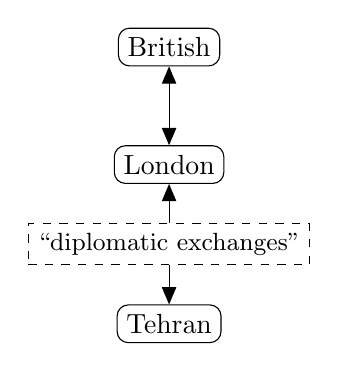
\begin{tikzpicture}
		\node[draw, dashed] (Diplo) {\small{``diplomatic exchanges''}} ;
		\node[draw, above=0.5cm of Diplo, rounded corners] (London) {London} ;
		\node[draw, rounded corners,above=of London] (British) {British} ;
		\node[draw, below=0.5cm of Diplo, minimum width=8.5mm, rounded corners] (Tehran) {Tehran} ;
		\edge [<->] {British} {London} ;
		\edge [<-] {London} {Diplo} ;
		\edge [->] {Diplo} {Tehran} ;		
	\end{tikzpicture}
	\caption{``A \entity{British} official, speaking anonymously because of the delicacy of the diplomatic exchanges between \entity{London} and \entity{Tehran}...''}
	\label{fig:nytimes-pgm1}
	\end{subfigure}
	\hfill
	\begin{subfigure}[t]{0.45\textwidth}
	\centering
	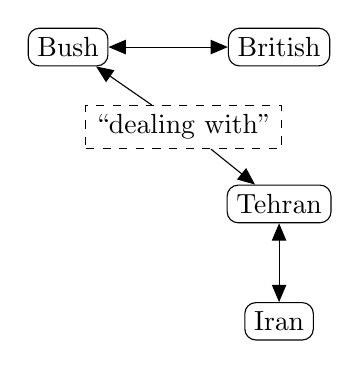
\begin{tikzpicture} %
		% Center
		\node[draw, dashed] (Dealing) {``dealing with''} ;
		\node[draw, below right=0.45cm and -0.7cm of Dealing, minimum width=8.5mm, rounded corners] (Tehran) {Tehran} ; %
		\node[left=1.5cm of Tehran] (Bushp) {\phantom{Bush}} ;
		\node[draw, rounded corners,above=1.5cm of Bushp] (Bush) {Bush} ;
		\node[draw, rounded corners, above=1.5cm of Tehran] (British) {British} ;
		\node[draw, rounded corners, below=of Tehran] (Iran) {Iran} ;
		% Emission
		\edge [<->] {Bush} {British} ;
		\edge [<->] {Tehran} {Iran} ;
		\edge [<-] {Bush} {Dealing} ;
		\edge [->] {Dealing} {Tehran} ;
	\end{tikzpicture}
	\caption{``The \entity{Bush} administration said Thursday that the release of 15 \entity{British} sailors and marines held by \entity{Iran} for two weeks created no new openings in dealing with \entity{Tehran}...''}
	\label{fig:nytimes-pgm2}
	\end{subfigure}
	\vspace{0.1cm}
	\begin{subfigure}[t]{0.45\textwidth}
		\centering
		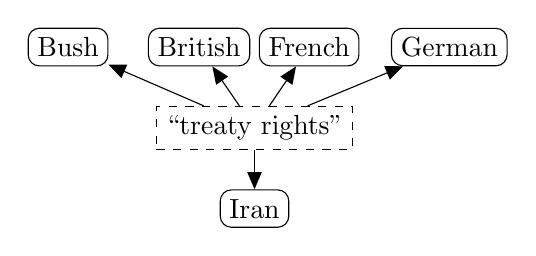
\begin{tikzpicture}
			\node[draw, dashed] (Treaty) {``treaty rights''} ;
			\node[draw, rounded corners, below=0.5cm of Treaty] (Iran) {Iran} ;
			\node[draw, rounded corners,above left=0.5cm and -1.2cm of Treaty] (British) {British} ;
			\node[draw, rounded corners,left=0.5cm of British] (Bush) {Bush} ;
			\node[draw, above right=0.5cm and -1.2cm of Treaty, minimum width=8.5mm, rounded corners] (French) {French} ; %
			\node[draw, rounded corners, right=0.4cm of French] (German) {German} ;
			\edge [<-] {Bush} {Treaty} ;
			\edge [<-] {British} {Treaty} ;
			\edge [<-] {French} {Treaty} ;
			\edge [<-] {German} {Treaty} ;
			\edge [->] {Treaty} {Iran} ;
		\end{tikzpicture}
		\caption{``By deceiving the nuclear agency about its activities, President \entity{Bush} and \entity{British}, French and German officials say, \entity{Iran} has given up whatever treaty rights it once enjoyed.''}
		\label{fig:nytimes-pgm3}
	\end{subfigure}
	\hfill
	\begin{subfigure}[t]{0.45\textwidth}
		\centering
		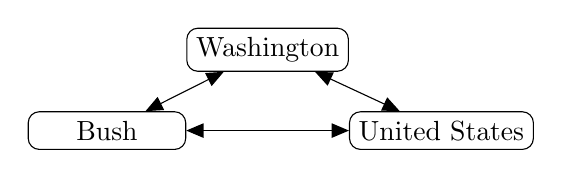
\begin{tikzpicture} %
				% Center
				\node[draw, rounded corners] (Washington) {Washington} ;
				\node[draw, rounded corners,below left=0.5cm and 0cm of Washington,minimum width=20mm] (Bush) {Bush} ;
				\node[draw, rounded corners,below right=0.5cm and 0cm of Washington] (US) {United States} ;
				
				% Emission
				\edge [<->] {Washington} {Bush} ;
				\edge [<->] {Washington} {US} ;
				\edge [<->] {Bush} {US} ;
			\end{tikzpicture}
			\caption{``Asserting \entity{Washington}'s determination to protect Japan and South Korea, its principal allies in the region, Mr. \entity{Bush} said the \entity{United States} `will meet the full range of our deterrent and security commitments.'{}''}
			\label{fig:nytimes-pgm4}
	\end{subfigure}
	\caption{Graphical models of the relationships which context-sensitive text-analysis algorithms can infer from sentences (1) through (4) above.}
	\label{fig:nytimes-pgm14}
\end{figure}

\begin{figure}[ht!]
	\centering
	\begin{subfigure}[t]{0.45\textwidth}
	\centering
	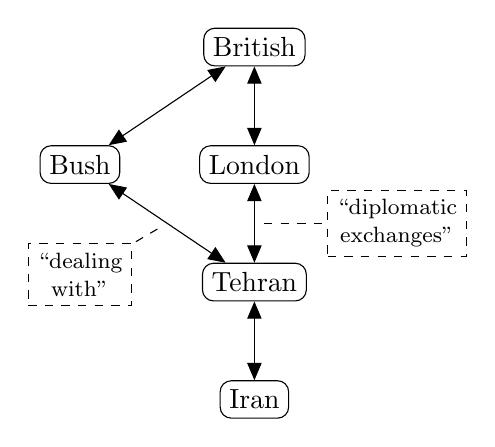
\begin{tikzpicture} %
		% Center
		\node[draw, rounded corners] (Bush) {Bush} ;
		\node[draw, rounded corners,right=of Bush] (London) {London} ;
		\node[draw, rounded corners,above=of London] (British) {British} ;
		\node[draw, below=of London, minimum width=8.5mm, rounded corners] (Tehran) {Tehran} ; %
		\node[draw, rounded corners, below=of Tehran] (Iran) {Iran} ;
		\edge [<->] {Bush} {British} ;
		% Diplo label
		%\node [above=0.33cm of Tehran] (Diplol) {} ;
		\node (Diplol) at ($(Tehran)!0.5!(London)$) {} ;
		\node [draw, dashed, right=0.8cm of Diplol] (Diplo) {\footnotesize\shortstack{``diplomatic\\exchanges''}} ;
		
		\edge [<->] {Tehran} {Iran} ;
		\edge [<->] {Bush} {Tehran} ;
		% Bush-Tehran label
		\node (Dealingl) at ($(Bush)!0.5!(Tehran)$) {} ;
		\node [draw, dashed, below=0.75cm of Bush] (Dealing) {\footnotesize\shortstack{``dealing\\with''}} ;
		\edge [<->] {London} {Tehran} ;
		\edge [<->] {British} {London} ;
		\edge [-,dashed] {Diplol} {Diplo} ;
		\edge [-,dashed] {Dealingl} {Dealing} ;
	\end{tikzpicture}
	\caption{The systematic merging of the networks in Figures \ref{fig:nytimes-pgm1} and \ref{fig:nytimes-pgm2}.}
	\label{fig:nytimes-pgm5}
	\end{subfigure}
	\hfill
	\begin{subfigure}[t]{0.45\textwidth}
	\centering
	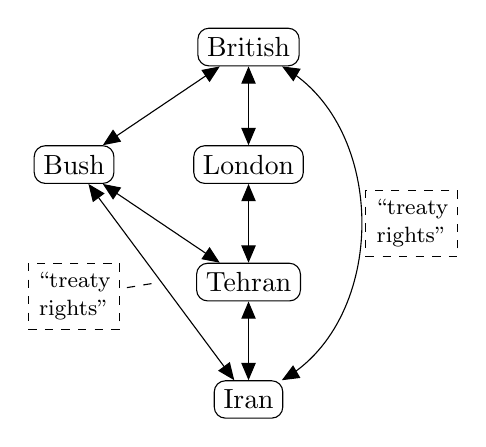
\begin{tikzpicture} %
		% Center
		\node[draw, rounded corners] (Bush) {Bush} ;
		\node[draw, rounded corners,right=of Bush] (London) {London} ;
		\node[draw, rounded corners,above=of London] (British) {British} ;
		\node[draw, below=of London, minimum width=8.5mm, rounded corners] (Tehran) {Tehran} ; %
		\node[draw, rounded corners, below=of Tehran] (Iran) {Iran} ;
		\edge [<->] {Bush} {British} ;
		\edge [<->] {Tehran} {Iran} ;
		\edge [<->] {Bush} {Tehran} ;
		\edge [<->] {London} {Tehran} ;
		\edge [<->] {British} {London} ;
		\edge [<->] {Bush} {Iran} ;
		% Bush-Iran label
		\node (Treatyl) at ($(Bush)!0.5!(Iran)$) {} ;
		\node [draw, dashed, below=1cm of Bush] (Treaty) {\footnotesize\shortstack{``treaty\\rights''}} ;
		%\edge [<->, bend left=90,looseness=1.2] {British} {Iran} ;
		\edge [-,dashed] {Treatyl} {Treaty} ;
		\path[<->]          (British)  edge   [bend left=60]   node[midway,right,draw,dashed,xshift=0.05cm] {\footnotesize\shortstack{``treaty\\rights''}} (Iran);
		% British-Iran label
		%\node (BTreatyl) at ($(London)!0.5!(Tehran)$) {} ;
		%\node [draw, dashed, right=1cm of BTreatyl] (BTreaty) {\footnotesize\shortstack{``treaty\\rights''}} ;
		%\edge [<->, bend left=90,looseness=1.2] {British} {Iran} ;
		%\edge [-,dashed] {BTreatyl} {BTreaty} ;
	\end{tikzpicture}
	\caption{The network formed by incorporating the information in Figure \ref{fig:nytimes-pgm3} into the network of panel (a).}
	\label{fig:nytimes-pgm6}
\end{subfigure}
\caption{An illustration of how, after constructing the individual-sentence context networks in Figure \ref{fig:nytimes-pgm14}, the algorithm can systematically merge the information across sentences, eventually producing the final corpus-wide network shown in Figure \ref{fig:nytimes-pgmfinal}.}
\label{fig:nytimes-pgm57}
\end{figure}

\begin{figure}[ht!]
	\centering
	\tikz{ %
		% Center
		\node[draw, rounded corners] (Bush) {Bush} ;
		\node[below=of Bush] (Bushp) {\phantom{Bush}} ;
		\node[draw, rounded corners,left=of Bushp] (Wash) {Washington} ;
		\node[draw, rounded corners,below=of Wash] (US) {United States} ;
		\node[draw, rounded corners,right=of Bush] (London) {London} ;
		\node[draw, rounded corners,above=of London] (British) {British} ;
		\node[draw, below=of London, minimum width=8.5mm, rounded corners] (Tehran) {Tehran} ; %
		\node[draw, rounded corners, below=of Tehran] (Iran) {Iran} ;
		
		% Emission
		\edge [<->] {Bush} {British} ;
		\edge [<->] {Tehran} {Iran} ;
		\edge [<->] {Bush} {Tehran} ;
		\edge [<->] {London} {Tehran} ;
		\edge [<->] {British} {London} ;
		\edge [<->] {Bush} {Iran} ;
		%\edge [<->] {British} {Iran} ;
		\edge [<->] {Bush} {Wash} ;
		\edge [<->] {Bush} {US} ;
		\edge [<->] {Wash} {US} ;
	}
	\caption{The final corpus-wide contextual network, combining all information from the individual networks in Figure \ref{fig:nytimes-pgm14} (edge labels omitted for clarity).}
	\label{fig:nytimes-pgmfinal}
\end{figure}


%\begin{enumerate}
%	\item (British <-> London) <-(diplomatic exchanges)-> Tehran
%	\item Bush <-> British <-(dealing with)-> Tehran -> Iran
%	\item Bush <-> British <-> French <-> German <-(treaty rights)-> Iran
%\end{enumerate}
The meaningful spatial positions of the learned vectors, moreover, give rise to a type of transitive property allowing us to infer information that is \textit{never} stated in the corpus, directly or indirectly. To see this, note how in Figure \ref{fig:nyt-vectors} one can travel from the $\vv{\texttt{Russia}}$ vector to the $\vv{\texttt{Kyiv}}$ vector via many different pathways, for example by:
	\begin{enumerate}
		\item[(a)] Following the $\vv{\textsf{Invaded}}$ vector to $\vv{\texttt{Ukraine}}$ and then following the $\vv{\textsf{Capital-Of}}$ vector to $\vv{\texttt{Kyiv}}$,
		\item[(b)] following the $\vv{\textsf{Capital-Of}}$ vector to $\vv{\texttt{Moscow}}$ and then following the $\vv{\textsf{Invaded}}$ vector to $\vv{\texttt{Kyiv}}$, or
		\item[(c)] Following the $\vv{\textsf{Leader-Of}}$ vector to $\vv{\texttt{Putin}}$, the $\vv{\textsf{Invaded}}$ vector to $\vv{\texttt{Zelensky}}$, the $\vv{\textsf{Leader-Of}}$ vector in the opposite direction to $\vv{\texttt{Ukraine}}$, and finally the $\vv{\textsf{Capital-Of}}$ vector to $\vv{\texttt{Kyiv}}$.
	\end{enumerate}
We illustrate this multitude of paths in Figure \ref{fig:nyt-paths}, where the pathways described by (a), (b), and (c) above are colored and labeled accordingly.
	
For example, having learned the aforementioned $\vv{\textsf{Capital-Of}}$ vector based on the respective contexts in which ``U.S.'' and ``Washington'' were used in the corpus, one could then add this vector to the vector for the entity \entity{Poland} to obtain the vector for \entity{Warsaw}, even if the corpus contained no explicit statements about Warsaw being the capital of Poland. Typically this is made possible by the algorithm's ability to pick up on subtle contextual patterns, like the fact that capital cities of a given country are often the most frequently-mentioned cities in stories about those countries. Thus, for example, the embedding for \entity{Ulaanbaatar} could occupy a similar position relative to \entity{Mongolia} as \entity{Warsaw} does to \entity{Poland}, even without the former appearing together in an explicit ``capital of'' context in the corpus, on account more simply of their common co-occurrence.

%The embedding spaces constructed by these algorithms, in other words, mirror the types of fairly complex inferences humans are able to make from a corpus:
%\begin{enumerate}
%	\item ``\entity{U.S.} officials are set to meet with \entity{Argentine} leaders next week in \entity{Buenos Aires}...''
%	\item ``IMF officials traveled to Buenos Aires on Monday...''
%	\item ``Debt restructuring talks between Argentina and the IMF broke down Wednesday...''
%	\item ``The Buenos Aires regime has suffered a legitimacy crisis since Argentina defaulted on its foreign debt at the end of 2001...''
%\end{enumerate}
	
% Then, since these vectors also respect transitivity, one can infer information 
It is in their ability to capture meaningful semantic relationships like these---an ability extending even to relationships never explicitly mentioned within a corpus---that we argue for understanding word embedding algorithms as methods for inferring and studying the ``geometry of political discourse''.
	
%%% Full NYTimes figure

\begin{figure}[ht!]
	\centering
	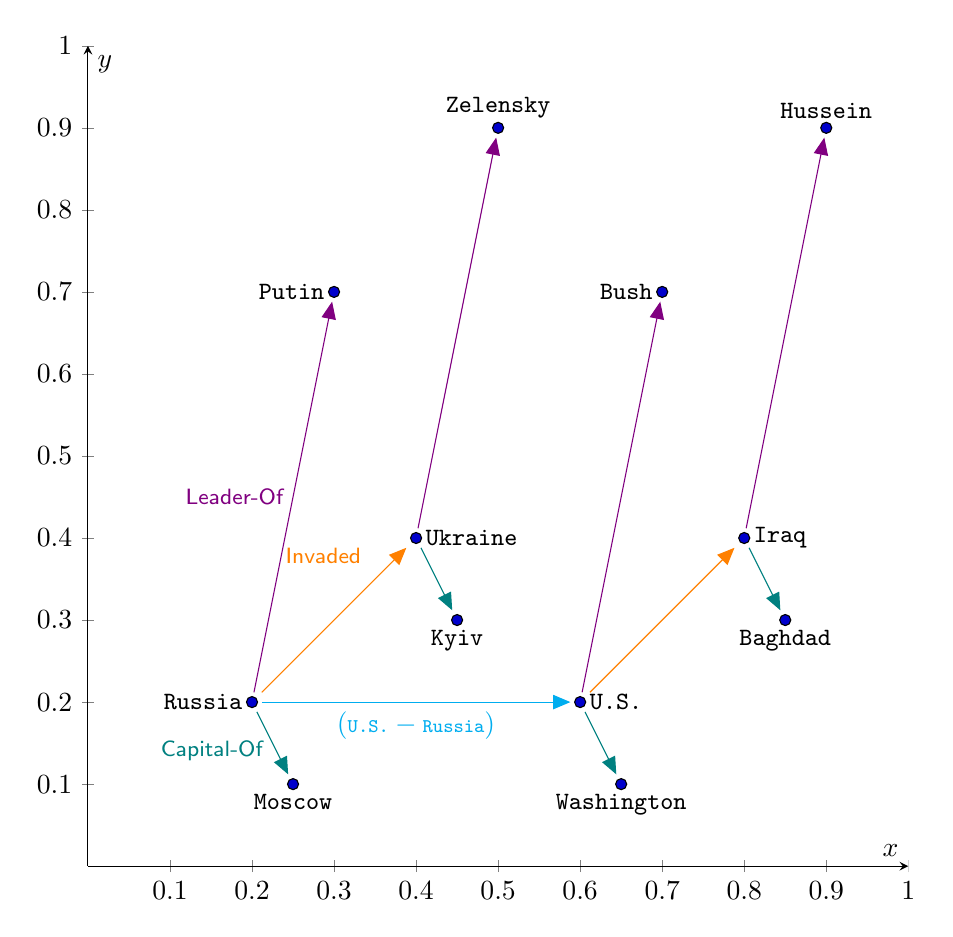
\begin{tikzpicture}
		\begin{axis}[axis lines=center,
			%view={28}{22},
			xmin=0, xmax=1, ymin=0, ymax=1,
			%xtick={0,1},ytick={0,1.0},
			xlabel=$x$,ylabel=$y$,width=12cm,height=12cm]
			\addplot+[only marks,point meta=explicit symbolic, nodes near coords,black] coordinates 
			{
				% Putin
				(0.3,0.7)[]
				% Russia
				(0.2,0.2)[]
				% Moscow
				(0.25,0.1)[]
				% Ukraine
				(0.4,0.4)[]
				% Kyiv
				(0.45,0.3)[]
				% Zelensky
				(0.5,0.9)[{\small$\entvecpgf{Zelensky}$}]
				% Bush
				(0.7,0.7)[]
				% US
				(0.6,0.2)[]
				% Washington
				(0.65,0.1)[]
				% Iraq
				(0.8,0.4)[]
				% Baghdad
				(0.85,0.3)[]
				% Hussein
				(0.9,0.9)[{\small$\entvecpgf{Hussein}$}]
			};
			%\node[anchor=west] (source) at (axis cs:0.0,0.0){};
			% Russia + Label
			\node (russia) at (axis cs:0.2,0.2){};
			\node[anchor=east] (russial) at (axis cs:0.2,0.2){{\small$\entvecpgf{Russia}$}};
			% Moscow + Label
			\node (moscow) at (axis cs:0.25,0.1){};
			\node[anchor=north] (moscowl) at (axis cs:0.25,0.1){{\small$\entvecpgf{Moscow}$}};
			% Ukraine + Label
			\node (ukraine) at (axis cs:0.4,0.4){};
			\node[anchor=west] (ukrainel) at (axis cs:0.4,0.4){{\small$\entvecpgf{Ukraine}$}};
			% Kyiv + Label
			\node (kyiv) at (axis cs:0.45,0.3){};
			\node[anchor=north] (kyivl) at (axis cs:0.45,0.3){{\small$\entvecpgf{Kyiv}$}};
			% Putin + Label
			\node (putin) at (axis cs:0.3,0.7){};
			\node[anchor=east] (putinl) at (axis cs:0.3,0.7){{\small$\entvecpgf{Putin}$}};
			% Zelensky
			\node (zelen) at (axis cs:0.5,0.9){};
			% US + Label
			\node (us) at (axis cs:0.6,0.2){};
			\node[anchor=west] (usl) at (axis cs:0.6,0.2){{\small$\entvecpgf{U.S.}$}};
			% Washington + Label
			\node (wash) at (axis cs:0.65,0.1){};
			\node[anchor=north] (washl) at (axis cs:0.65,0.1){{\small$\entvecpgf{Washington}$}};
			% Iraq + Label
			\node (iraq) at (axis cs:0.8,0.4){};
			\node[anchor=west] (iraql) at (axis cs:0.8,0.4){{\small$\entvecpgf{Iraq}$}};
			% Baghdad + Label
			\node (baghdad) at (axis cs:0.85,0.3){};
			\node[anchor=north] (baghdadl) at (axis cs:0.85,0.3){{\small$\entvecpgf{Baghdad}$}};
			% Bush + Label
			\node (bush) at (axis cs:0.7,0.7){};
			\node[anchor=east] (bushl) at (axis cs:0.7,0.7){{\small$\entvecpgf{Bush}$}};
			% Hussein
			\node (hussein) at (axis cs:0.9,0.9){};
			%%% Arrow labels
			% Invaded
			\node[anchor=north west,color=orange] (invaded) at (axis cs:0.229,0.4){{\footnotesize$\relvecpgf{Invaded}$}};
			% US-Russia
			\node[anchor=north,color=cyan] (usmrus) at (axis cs:0.4,0.2){$\left(\vv{\scriptsize{\texttt{U.S.}}}-\vv{\scriptsize{\texttt{Russia}}}\right)$};
			% Leader
			\node[anchor=east,color=violet] (leader) at (axis cs:0.25,0.45) {{\footnotesize$\relvecpgf{Leader-Of}$}};
			% Capital
			\node[anchor=east, color=teal] (capital) at (axis cs:0.225,0.14) {{\footnotesize$\relvecpgf{Capital-Of}$}};
			\draw[->,color=orange](russia)--(ukraine);
			\draw[->,color=violet](russia)--(putin);
			\draw[->,color=teal](russia)--(moscow);
			\draw[->,color=cyan](russia)--(us);
			\draw[->,color=violet](ukraine)--(zelen);
			\draw[->,color=teal](ukraine)--(kyiv);
			%\draw[->,color=orange](putin)--(zelen);
			\draw[->,color=orange](us)--(iraq);
			\draw[->,color=violet](us)--(bush);
			\draw[->,color=teal](us)--(wash);
			\draw[->,color=violet](iraq)--(hussein);
			\draw[->,color=teal](iraq)--(baghdad);
			%\draw[->,color=orange](bush)--(hussein);
		\end{axis}
	\end{tikzpicture}
	\caption{A visualization of the ``analogical math'' which can be performed within word embedding spaces, due to their ability to capture multiple \textit{types} of word-word relationships in the form of distances ranging over multiple dimensions: entity vectors are typeset in fixed-width font ($\entvec{Entity}$), while relational vectors are typeset in serif font ($\relvec{Relation}$). The vector from $\entvec{Russia}$ to $\entvec{U.S.}$, a relational vector, is typeset in fixed-width font only to illustrate its mathematical form (i.e., that it is computed via the subtraction two entity vectors).}
	\label{fig:nyt-vectors}
\end{figure}

%%% NYTimes paths figure

\begin{figure}[ht!]
	\centering
	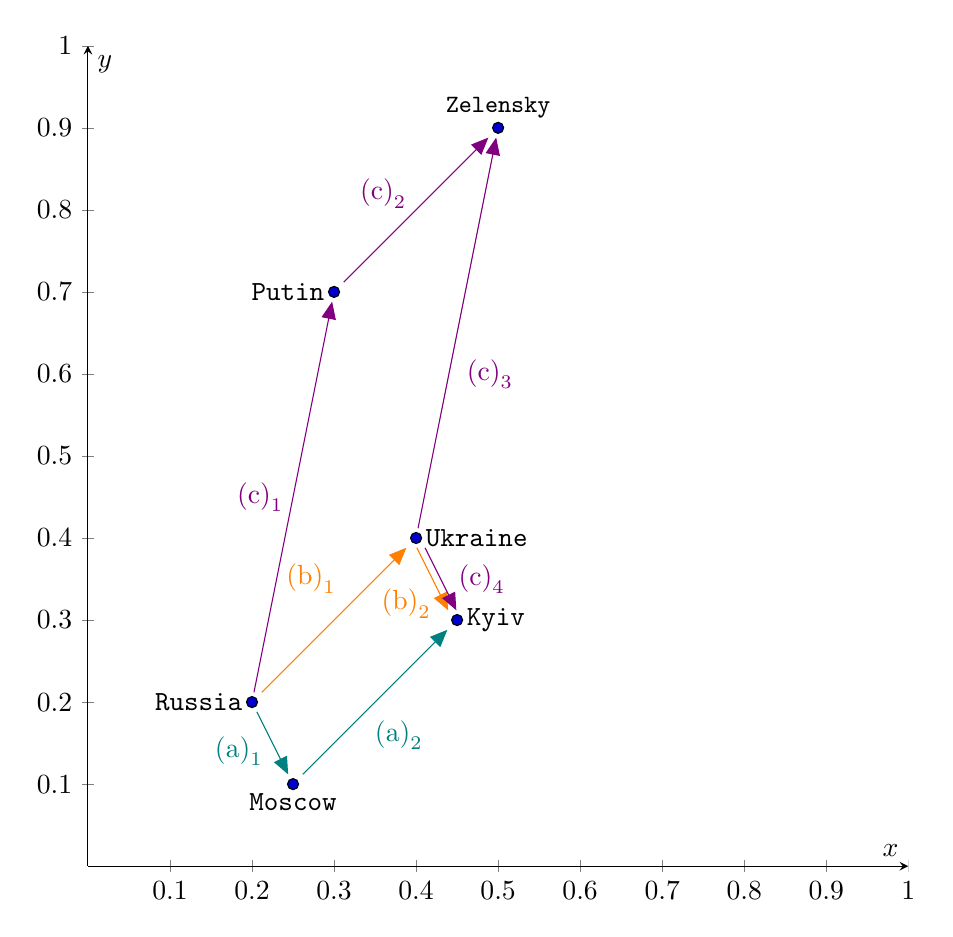
\begin{tikzpicture}
		\begin{axis}[axis lines=center,
			%view={28}{22},
			xmin=0, xmax=1, ymin=0, ymax=1,
			%xtick={0,1},ytick={0,1.0},
			xlabel=$x$,ylabel=$y$,width=12cm,height=12cm]
			\addplot+[only marks,point meta=explicit symbolic, nodes near coords,black] coordinates 
			{
				% Putin
				(0.3,0.7)[]
				% Russia
				(0.2,0.2)[]
				% Moscow
				(0.25,0.1)[]
				% Ukraine
				(0.4,0.4)[]
				% Kyiv
				(0.45,0.3)[]
				% Zelensky
				(0.5,0.9)[$\vv{\small{\texttt{Zelensky}}}$]
			};
			%\node[anchor=west] (source) at (axis cs:0.0,0.0){};
			% Russia + Label
			\node (russia) at (axis cs:0.2,0.2){};
			\node[anchor=east] (russial) at (axis cs:0.2,0.2){$\entvecpgf{Russia}$};
			% Moscow + Label
			\node (moscow) at (axis cs:0.25,0.1){};
			\node[anchor=north] (moscowl) at (axis cs:0.25,0.1){$\entvecpgf{Moscow}$};
			% Ukraine + Label
			\node (ukraine) at (axis cs:0.4,0.4){};
			\node (ukrainewest) at (axis cs:0.395,0.4){};
			\node (ukraineeast) at (axis cs:0.405,0.4){};
			\node[anchor=west] (ukrainel) at (axis cs:0.4,0.4){$\entvecpgf{Ukraine}$};
			% Kyiv + Label
			\node (kyiv) at (axis cs:0.45,0.3){};
			\node (kyivwest) at (axis cs:0.445,0.3){};
			\node (kyiveast) at (axis cs:0.455,0.3){};
			\node[anchor=west] (kyivl) at (axis cs:0.45,0.3){$\entvecpgf{Kyiv}$};
			% Putin + Label
			\node (putin) at (axis cs:0.3,0.7){};
			\node[anchor=east] (putinl) at (axis cs:0.3,0.7){$\entvecpgf{Putin}$};
			% Zelensky
			\node (zelen) at (axis cs:0.5,0.9){};
			%\node (zelenl) at ()
			%%% Arrow labels
			% (b)_1
			\node[anchor=north west,color=orange] (b1) at (axis cs:0.23,0.38){$\text{(b)}_1$};
			% (b)_2
			\node[anchor=east, color=orange] (b2) at (axis cs:0.43,0.32){$\text{(b)}_2$};
			% (c)_1
			\node[anchor=east,color=violet] (c1) at (axis cs:0.25,0.45) {$\text{(c)}_1$};
			% (c)_2
			\node[anchor=east, color=violet] (c2) at (axis cs:0.4,0.82) {$\text{(c)}_2$};
			% (c)_3
			\node[anchor=west, color=violet] (c3) at (axis cs:0.45,0.6) {$\text{(c)}_3$};
			% (c)_4
			\node[anchor=west, color=violet] (c4) at (axis cs:0.44,0.35) {$\text{(c)}_4$};
			% Capital
			%\node[anchor=east, color=teal] (capital) at (axis cs:0.225,0.14) {$\relvecpgf{Capital}$};
			% (a)_1
			\node[anchor=east, color=teal] (a1) at (axis cs:0.225,0.14) {$\text{(a)}_1$};
			% (a)_2
			\node[anchor=east, color=teal] (a2) at (axis cs:0.42,0.16) {$\text{(a)}_2$};
			\draw[->,color=orange](russia)--(ukraine);
			\draw[->,color=violet](russia)--(putin);
			\draw[->,color=teal](russia)--(moscow);
			\draw[->,color=violet](ukraine)--(zelen);
			\draw[->,color=orange](ukrainewest)--(kyivwest);
			\draw[->,color=violet](ukraineeast)--(kyiveast);
			\draw[->,color=teal](moscow)--(kyiv);
			\draw[->,color=violet](putin)--(zelen);
		\end{axis}
	\end{tikzpicture}
	\caption{Visualizing three of the potential pathways by which one can move from the $\texttt{Russia}$ to the $\texttt{Kyiv}$ vectors.}
	\label{fig:nyt-paths}
\end{figure}
	
While we will dive into the details of these embedding algorithms more deeply in Section \ref{sec:meaning-context} below, to see \textit{how} they are able to capture these multi-layered semantic relationships, for now we conclude by re-emphasizing how understanding contextual embedding algorithms as \textit{computational implementations} of Firth's hypothesis thus ``completes the loop'' from computational linguistics to the Cambridge School and back: the contextual analysis advocated by Cambridge School scholars and carried out via a deep reading of a wide array of historical texts is precisely mirrored in the processes that generate these neural embedding spaces. And, as touched on above (a consideration which we will also discuss in more detail below), while embeddings restricted to the level of words are perhaps too lexically fine-grained to allow a general understanding of a text in the sense advocated by the Cambridge School, the move from contextual word embeddings up to contextual \textit{sentence} embeddings in recent years brings us significantly closer to the textual level of analysis, and offers hope that the types of methods used to aggregate information from the word to the sentence level could also bear fruit for the further aggregation of information up to the level of full texts within a corpus.

\section{Models of Meaning and Context}\label{sec:meaning-context}

\subsection{Constructing Contextual Fields}\label{sec:contextual-fields}

The key computational tool used throughout the studies in the remainder of this work is the contextual sentence embedding algorithm, a method for mapping linguistic units (words, phrases, sentences, documents) into geometric spaces based on their semantic content. In fact, there is no single ``embedding algorithm'', but rather a wide range of algorithms which transform various linguistic entities into points within a high-dimensional geometric space. Although our unit of analysis herein is a \textit{document} (e.g., a text, pamphlet, or letter), these documents are in general too long for a single embedding algorithm to handle -- state-of-the-art embedding algorithms like \BERT{} have an upper limit of 512 tokens that can be jointly encoded into a single high-dimensional vector. Thus we instead compute a separate embedding for each \textit{sentence} within a text using \texttt{SentenceTransformers} \parencite{reimers_sentencebert_2019}, then combine these sentence vectors into a single document vector via mean pooling. As a robustness check, however, we computed document-level embeddings via an experimental document embedding method called Longformer, described in \cite{beltagy_longformer_2020}, and obtained qualitatively similar results.
%(see Appendix \ref{app:longformer}).

%\begin{figure}[ht!]
%	\centering
%	\includegraphics[width=\textwidth]{./ch_methods/figs/dimensionality_reduction.jpeg}
%	\caption{Figure 1 from \cite{kozlowski_geometry_2019}, illustrating how word embedding algorithms solve the problem of how to best capture the relationships between words and their contexts while restricting the representation of words to only 3 dimensions.}
%	\label{fig:dim-reduction}
%\end{figure}

Turning to the issue of \textit{how} exactly the semantic information in a text is given a geometric interpretation: at the most basic level, sentence embedding algorithms take every word appearing in a corpus and represent them as points within a geometric space, such that words which are used in similar contexts\footnote{Although ``context'' can be operationalized in different ways based on what information a user hopes to extract, in our case the context of a word $w$ in a sentence $S$ is defined to be the set of $n$ words appearing before and after $w$ in the sentence. For example, if $S$ is ``\texttt{The sleepy grey cat likes salmon.}'', and $w$ is ``\texttt{cat}'', then the context of $w$ with $n = 2$ would be the set $\{\texttt{sleepy}, \texttt{grey}, \texttt{likes}, \texttt{salmon}\}$.} will be placed closer together in the space than sentences which use dissimilar words and/or dissimilar contexts around these words. In this way, computers can begin to reason about semantic relationships between words by analyzing the geometric properties of these constructed spaces, as in Figure \ref{fig:cosine-sim}.

\begin{figure}[ht!]
	\centering
	\begin{subfigure}{0.45\linewidth}
	\centering
	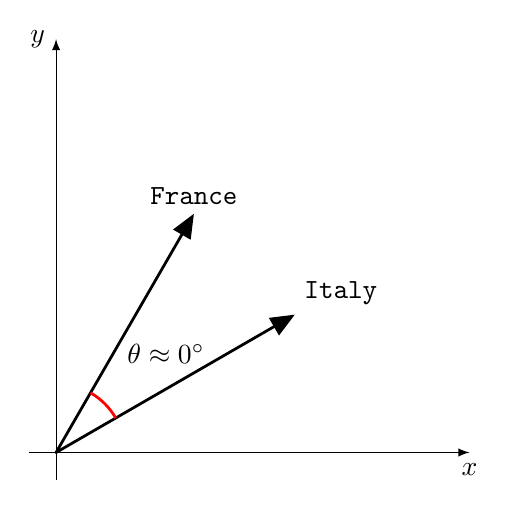
\begin{tikzpicture}[scale=3.5]
		%\tkzInit
		\tkzInit[xmin=-0.1,xmax=1,ymin=-0.1,ymax=1]
		%\tkzGrid
		\tkzDrawX[>=latex] \tkzDrawY[>=latex]
		\tkzDefPoint(0,0){O}
		\tkzDefPoint(0.5,0.866){F}
		\tkzDefPoint(0.866,0.5){I}
		%\tkzDrawPoints(O,I,F)
		%\tkzLabelPoints(O,I,F)
		\tkzDrawSegment[->,line width=1](O,I)
		\tkzDrawSegment[->,line width=1](O,F)
		\tkzLabelPoint[above](F){\entpgf{France}}
		\tkzLabelPoint[above right](I){\entpgf{Italy}}
		% New
		% Label POA angle
		% New triangle angles
		\tkzMarkAngle[size=0.25,color=red,line width=1](I,O,F)
		\tkzLabelAngle[above right=0mm and -2.2mm,pos=0.4](I,O,F){$\theta \approx 0^\circ$}
		%\tkzLabelAngle(T,A,O){$x_3$}
	\end{tikzpicture}
\end{subfigure}
\begin{subfigure}{0.45\linewidth}
	\centering 
	\begin{tikzpicture}[scale=3]
		%\tkzInit
		\tkzInit[xmin=-0.1,xmax=1,ymin=-1,ymax=1]
		%\tkzGrid
		\tkzDrawX[>=latex] \tkzDrawY[>=latex]
		\tkzDefPoint(0,0){O}
		\tkzDefPoint(0.707,0.707){B}
		\tkzDefPoint(0.707,-0.707){C}
		%\tkzDrawPoints(O,I,F)
		%\tkzLabelPoints(O,I,F)
		\tkzDrawSegment[->,line width=1](O,B)
		\tkzDrawSegment[->,line width=1](O,C)
		\tkzLabelPoint[above](B){\entpgf{Ball}}
		\tkzLabelPoint[above right](C){\entpgf{Crocodile}}
		% New
		% Label POA angle
		% New triangle angles
		\tkzMarkAngle[size=0.2,color=red,line width=1](C,O,B)
		\tkzLabelAngle[above right,pos=0.2](C,O,B){$\theta \approx 90^\circ$}
		%\tkzLabelAngle(T,A,O){$x_3$}
	\end{tikzpicture}
\end{subfigure}
\caption{The word-level linguistic intuitions which, by constructing an appropriate geometric space, can be quantitatively measured by way of the Cosine Similarity metric: (a) On the left, \entity{France} and \entity{Italy} are quite similar, so that $\theta$ is close to $0^\circ$, and $\cos(\theta)$ is close to $1$. (b) On the right, \entity{Ball} and \entity{Crocodile} are not similar, so that $\theta$ is close to $90^\circ$, and $\cos(\theta)$ is close to $0$.}
\label{fig:cosine-sim}
\end{figure}

By implementing this micro-level property---that is, the property that words or phrases which share similar contexts should be close together in the generated geometric space---across an entire text corpus, what emerges at the macro level is a landscape of the words and phrases in the corpus within which distinct regions can be identified which correspond to our intuitions about semantic meaning in human language. For example, Figure \ref{fig:xlang-embeddings} visualizes a cross-lingual embedding space where each node is colored based on what part of speech it represents, demonstrating how these embedding algorithms, despite focusing solely on micro-level (i.e., word- or phrase-level) similarity properties, naturally give rise to geometric spaces which capture macro-level properties of human languages.

\begin{figure}[ht!]
	\centering
	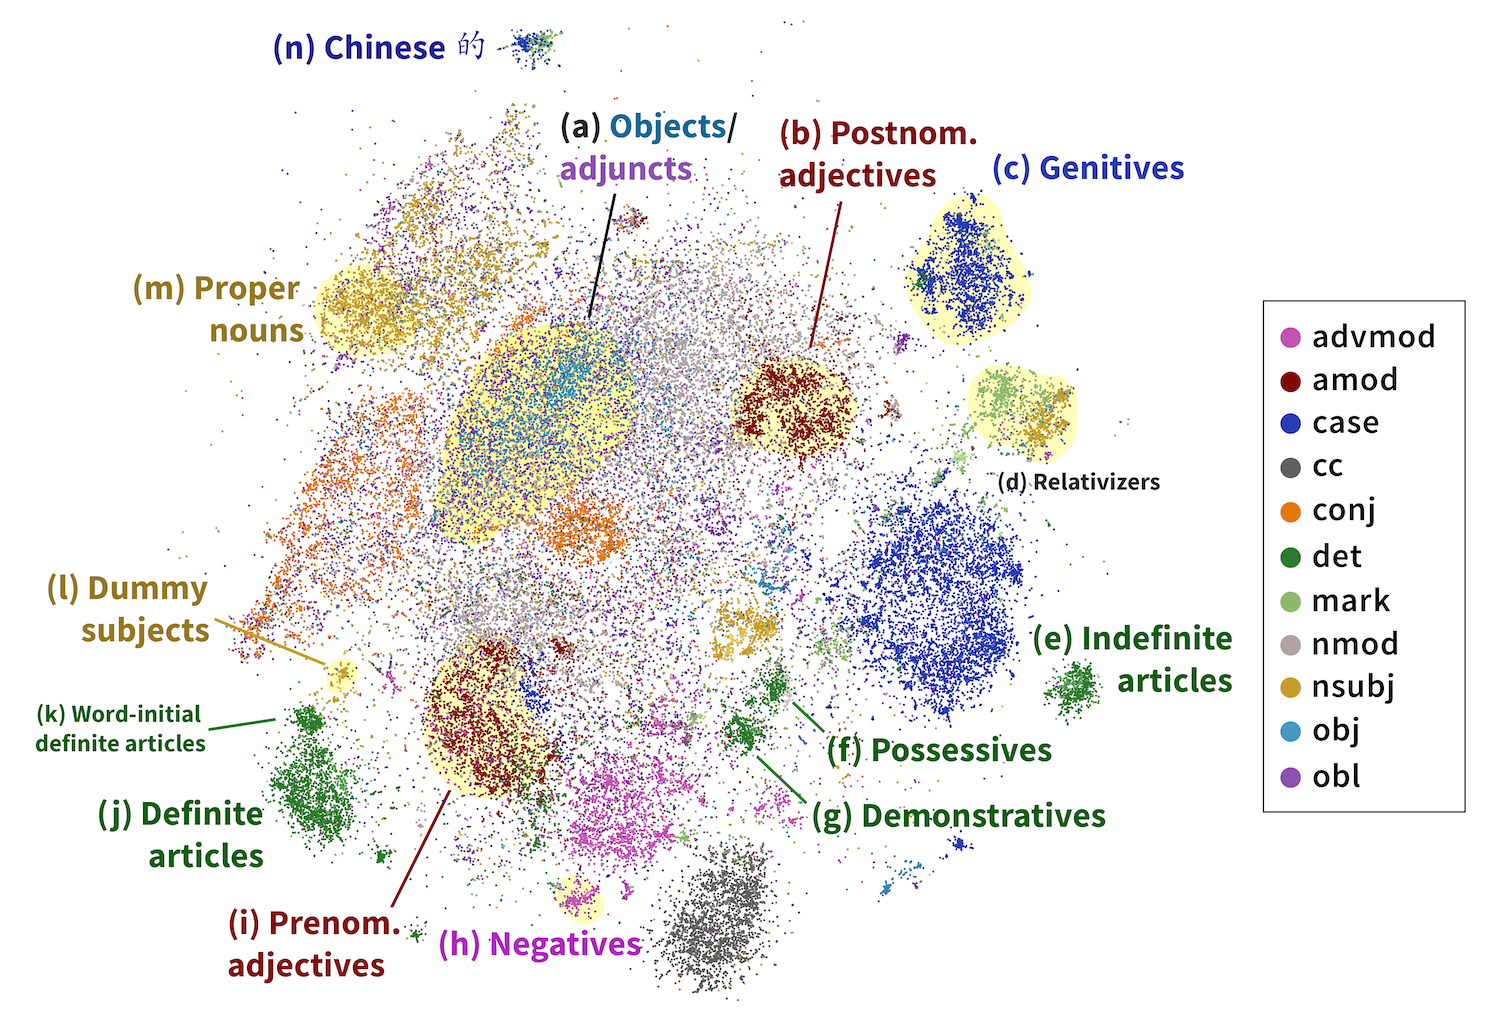
\includegraphics[width=\textwidth]{../figs/xlang_embeddings.png}
	\caption{An example of the higher-level properties of language which naturally emerge when an embedding algorithm computes \textit{word-level} contextual-semantic similarities (that is, moves the points for words which occur in similar contexts closer together) across a large corpus of text from many different languages. (From \cite{chi_finding_2020}, Figure 6)}
	\label{fig:xlang-embeddings}
\end{figure}

%\begin{itemize}
%	\item Civill Law, Is to every Subject, those Rules, which the Common-wealth hath Commanded him, by Word, Writing, or other sufficient Sign of the Will, to make use of, for the Distinction of Right, and Wrong; that is to say, of what is contrary, and what is not contrary to the Rule.
%	\item Liberty, or Freedome, signifieth (properly) the absence of Opposition; (by Opposition, I mean externall Impediments of motion;) and may be applyed no lesse to Irrationall, and Inanimate creatures, than to Rationall.
%\end{itemize}

% Hobbes example
\begin{figure}[ht!]
	\centering
	\[\arraycolsep=1.8pt\def\arraystretch{1.2}
	\begin{blockarray}{c@{\hspace{2mm}}c@{\hspace{1.5mm}}c@{\hspace{2mm}}c@{\hspace{2mm}}c@{\hspace{2mm}}c@{\hspace{1.8mm}}c@{\hspace{1.8mm}}c}
		& \texttt{\small{law}} & \texttt{\small{power}} & \texttt{\small{soveraign}} & \texttt{\small{christ}} & \cdots & \texttt{\small{justice}} \\
		\begin{block}{c@{\hspace{2mm}}[c@{\hspace{1.5mm}}c@{\hspace{2mm}}c@{\hspace{2mm}}c@{\hspace{2mm}}c@{\hspace{1.8mm}}c@{\hspace{1.8mm}}c]}
			\texttt{\small{law}} & 2257 & 376 & 560 & 74 & \cdots & 100 \\
			\texttt{\small{power}} & 376 & 1071 & 624 & 80 & \cdots & 36 \\
			\texttt{\small{soveraign}} & 560 & 624 & 983 & 32 & \cdots & 38 \\
			\texttt{\small{christ}} & 74 & 80 & 32 & 727 & \cdots & 0 \\
			\vdots & \vdots & \vdots & \vdots & \vdots & \ddots & \vdots \\
			\texttt{\small{justice}} & 100 & 36 & 38 & 0 & \cdots & 143 \\
		\end{block}
	\end{blockarray} 
	%\leadsto
	\approx
	\begin{blockarray}{c@{\hspace{2mm}}c@{\hspace{2mm}}c}
		& x & y \\
		\begin{block}{c@{\hspace{2mm}}[r@{\hspace{2mm}}r]}
			\texttt{\small{law}} & 0.52 & 7.38 \\
			\texttt{\small{power}} & 0.54 & 6.04 \\
			\texttt{\small{soveraign}} & 0.35 & 10.92 \\
			\texttt{\small{christ}} & 8.03 & -6.53 \\
			\vdots & \vdots & \vdots \\
			\texttt{\small{justice}} & -0.22 & 10.50 \\
		\end{block}
	\end{blockarray}
	\times V %V^{\top}
	\]
	\caption{The mathematical operation (dimensionality reduction) by which we compress the \textit{full} set of word-context information in Hobbes' \textit{Leviathan} (the matrix on the left) into a smaller matrix of two-dimensional vectors (the rows in the right-side matrix) which best preserve contextual similarity. That is, similar rows in the left-side matrix will be mapped to close-by points in 2D space, with $(x,y)$ coordinates as given in the right-side matrix.}
\end{figure}
%\begin{figure}[ht!]
%	\begin{align*}
	%		\begin{bmatrix}
		%		\text{Liberty} & 2 & 0 & 0 & 3 & 0 & 2 & 7 & \cdots & 4 \\
		%		\text{Law} & 3 & 1 & 0 & 6 & 0 & 0 & 2 & \cdots & 0 \\
		%		\text{Subject} & 1 & 3 & 4 & 2 & 7 & 2 & 0 & \cdots & 9 \\
		%		\text{Common-wealth} & 7 & 0 & 1 & 0 & 3 & 0 & 7 & \cdots & 4 \\
		%		\text{Right} & 0 & 2 & 0 & 4 & 0 & 0 & 7 & \cdots & 0 \\
		%		\text{Wrong} & 0 & 0 & 0 & 0 & 0 & 0 & 0 & \cdots & 0 \\
		%			
		%		\end{bmatrix} \approx
	%		\begin{bmatrix}.3 & .1 & .0 \\ .1 & .3 & .4\end{bmatrix} \times \begin{bmatrix}.2 & .2 & .1 \\ .7 & .0 & .1\end{bmatrix}
	%	\end{align*}
%	\caption{Constructing a geometric space which embeds key terms from Hobbes' \textit{Leviathan}.}
%	\label{fig:hobbes-matrices}
%\end{figure}


% Kozlowski example
\begin{figure}[ht!]
	\centering
	\[\arraycolsep=1.8pt\def\arraystretch{1.2}
	\begin{blockarray}{c@{\hspace{4mm}}c@{\hspace{2mm}}c@{\hspace{2mm}}c@{\hspace{2mm}}c@{\hspace{2mm}}c@{\hspace{2mm}}c@{\hspace{2mm}}c@{\hspace{2mm}}c@{\hspace{2mm}}c}
		& ~~\rot{\textsf{\small{context 1}}} & \rot{\textsf{\small{context 2}}} & \rot{\textsf{\small{context 3}}} & \rot{\textsf{\small{context 4}}} & \rot{\textsf{\small{context 5}}} & \rot{\textsf{\small{context 6}}} & \rot{\textsf{\small{context 7}}} & \small{\cdots} & \rot{\small{\textsf{context}} $M$}~ \\
		\begin{block}{c[@{\hspace{4mm}}c@{\hspace{2mm}}c@{\hspace{2mm}}c@{\hspace{2mm}}c@{\hspace{2mm}}c@{\hspace{2mm}}c@{\hspace{2mm}}c@{\hspace{2mm}}c@{\hspace{2mm}}c]}
			\textsf{word 1} & 2 & 0 & 0 & 3 & 0 & 2 & 7 & \cdots & 4 \\
			\textsf{word 2} & 3 & 1 & 0 & 6 & 0 & 0 & 2 & \cdots & 0 \\
			\textsf{word 3} & 1 & 3 & 4 & 2 & 7 & 2 & 0 & \cdots & 9 \\
			\textsf{word 4} & 7 & 0 & 1 & 0 & 3 & 0 & 7 & \cdots & 4 \\
			\textsf{word 5} & 0 & 2 & 0 & 4 & 0 & 0 & 7 & \cdots & 0 \\
			\textsf{word 6} & 0 & 9 & 3 & 2 & 1 & 3 & 0 & \cdots & 0 \\	
			\textsf{word 7} & 2 & 0 & 0 & 1 & 0 & 5 & 1 & \cdots & 3 \\	
			\vdots & \vdots & \vdots & \vdots & \vdots & \vdots & \vdots & \vdots & \ddots & \vdots \\	
			\textsf{word~}N & 5 & 0 & 1 & 3 & 0 & 0 & 5 & \cdots & 3 \\
		\end{block}
		& \BAmulticolumn{9}{c}{\underbrace{\small\text{\phantom{C}Word-Context Matrix}\phantom{C}}_{N \times M}} \\
	\end{blockarray}
	\approx
	\begin{blockarray}{c@{\hspace{3mm}}c@{\hspace{2mm}}c}
		\rot{\phantom{\textsf{\small{context }$M$}}}x~ & ~y & z \\
		\begin{block}{[c@{\hspace{2mm}}c@{\hspace{2mm}}c]}
			.3 & .1 & .0 \\ .1 & .3 & .4 \\ .0 & .2 & .1 \\ .0 & .9 & .3 \\ .2 & .0 & .3 \\ .5 & .0 & .1 \\ .0 & .9 & .0 \\ \vdots & \vdots & \vdots \\ .2 & .1 & .3 \\
			% \undermat{\text{Word Vectors}}{.2 & .1 & .3} \\
		\end{block}
		\BAmulticolumn{3}{c}{\underbrace{\small\text{Word Vectors}}_{N \times 3}} \\
	\end{blockarray}
	%\substack{{\textstyle\;\times\;}\\~\\~}
	\times
	\begin{blockarray}{c@{\hspace{2mm}}c@{\hspace{2mm}}c@{\hspace{2mm}}c@{\hspace{2mm}}c@{\hspace{2mm}}c@{\hspace{2mm}}c@{\hspace{2mm}}c@{\hspace{2mm}}c}
		\BAmulticolumn{9}{c}{\phantom{\underbrace{\small\text{\phantom{Conte}Context Vectors}\phantom{Conte}}_{3 \times M}}} \\
		\BAmulticolumn{9}{c}{\vspace{-2.5mm}} \\
		%\BAnoalign{\centering Unlike ...}
		\begin{block}{[c@{\hspace{2mm}}c@{\hspace{2mm}}c@{\hspace{2mm}}c@{\hspace{2mm}}c@{\hspace{2mm}}c@{\hspace{2mm}}c@{\hspace{2mm}}c@{\hspace{2mm}}c]}
			.2 & .2 & .1 & .3 & .0 & .2 & .7 & \cdots & .4 \\
			.7 & .0 & .1 & .0 & .3 & .5 & .7 & \cdots & .4 \\
			.9 & .8 & .6 & .3 & .0 & .1 & .7 & \cdots & .0 \\
		\end{block}
		\BAmulticolumn{9}{c}{\underbrace{\small\text{\phantom{Conte}Context Vectors}\phantom{Conte}}_{3 \times M}} \\
	\end{blockarray}
	\]
	\caption{An example of the matrix decomposition procedure that word embedding algorithms implement, to solve the problem of \textit{retaining} information about word-context relationships while \textit{reducing} the $M$-dimensional representations of each word down to 3 dimensions. (Example adapted from \cite{kozlowski_geometry_2019}, Figure 1)}
	\label{fig:kozlowski-decomposition}
\end{figure}

To understand how exactly this text-to-geometric-space transformation works, Figure \ref{fig:kozlowski-decomposition} illustrates how the task can be represented as a mathematical problem which, when solved, produces precisely the desired semantic-capturing and context-sensitive geometric space. Given the \textit{full} set of contextual information about each word---that is, how many times the word appears in each possible context---the aim is to compress the information for each word into just 3 dimensions, such that words which appear in similar contexts will be close together when visualized in 3D space. Visualizing the 3D space generated in the figure, for example, word 5 will be very close to word $n$, as word 5 will be mapped to the coordinate $(x,y,z) = (.2,.0,.3)$, while word $n$ will be mapped to $(x,y,z) = (.2,.1,.3)$, so that they differ only by $0.1$ in the $y$ coordinate, as visualized in Figure \ref{fig:geometry-td}.

\begin{figure}[ht!]
	\centering
	\begin{tikzpicture}
		\begin{axis}[axis lines=center,
			view={28}{22},
			xmin=0, xmax=1.1,
			ymin=0, ymax=1.1,
			zmin=0, zmax=1.1,
			xtick={0,1},ytick={0,1.0},ztick={0,1.0},
			xlabel=$x$,ylabel=$y$,zlabel=$z$,
			x label style={anchor=west},
			y label style={at={(axis description cs:0.38,0.42)},anchor=north},
			z label style={anchor=south}
			]
			\addplot3+[only marks,point meta=explicit symbolic, nodes near coords] coordinates 
			{
				%(0.3,0.1,0.0)[Word 1]
				(0.1,0.3,0.4)[2]
				%(0.0,0.2,0.1)[3]
				(0.0,0.9,0.3)[4]
				(0.2,0.0,0.3)[5]
				(0.5,0.0,0.1)[6]
				%(0.0,0.9,0.0)[7]
				(0.2,0.1,0.3)[$n$]
			};
		\end{axis}
	\end{tikzpicture}
	\caption{A plot of the 3-dimensional word representations in Figure \ref{fig:kozlowski-decomposition}.}
	\label{fig:geometry-td}
\end{figure}

To see how powerful this dimensionality-reduction approach is, let's consider an extremely small corpus of four ``documents'', where each document is actually just a single 3-4 word sentence:
\begin{enumerate}
	\item \texttt{Green eggs are sweet.}
	\item \texttt{Ham is sour.}
	\item \texttt{Cats love sweet food.}
	\item \texttt{Dogs love sour food.}
\end{enumerate}
Taking the set of unique words\footnote{That is, the unique words after the \textit{function words} ``are'' and ``is'' have been removed. Standard practice in word embedding models is to remove all such function words, since they pertain to the \textit{syntax} rather than the semantic content of a given sentence. In other research applications, however, the syntactic structure of the sentences may be exactly what one is hoping to capture with these embeddings, in which case all \textit{non-}function words are removed. See \cite{mosteller_inference_1964} for a seminal application of this syntax-based analysis in the social sciences.}, and defining the context of a word to be the full sentence in which it appears, we obtain the Word-Context Matrix shown (along with the resulting two-dimensional embeddings) in Figure \ref{fig:eggs-matrix}. By examining the plot of the resulting two-dimensional embeddings in Figure \ref{fig:eggs-plot}, we can see that despite having a corpus of only four sentences (providing a total of 15 tokens) to infer information from, the method is already able to detect multiple semantic relationships: First, we see that it has captured the identical context-employment of \texttt{green} and \texttt{eggs}, by mapping them onto the same point in the 2D space. Second, we see that it has used the $x$-axis to separate two triangles of points, one representing the semantic relations involving \texttt{cat} and the other the semantic relations involving \texttt{dog}.

\begin{figure}[ht!]
\centering
	\[\arraycolsep=1.8pt\def\arraystretch{1.2}
	\begin{blockarray}{ccccccccc}
		& \rot{\texttt{\small{cats}}} & \rot{\texttt{\small{dogs}}} & \rot{\texttt{\small{eggs}}} & \rot{\texttt{\small{green}}} & \rot{\texttt{\small{ham}}} & \rot{\texttt{\small{love}}} & \rot{\texttt{\small{sour}}} & \rot{\texttt{\small{sweet}}} \\
		\begin{block}{c[cccccccc]}
\texttt{cats} & 1 & 0 & 0 & 0 & 0 & 1 & 0 & 1 \\
\texttt{dogs} & 0 & 1 & 0 & 0 & 0 & 1 & 1 & 0 \\
\texttt{eggs} & 0 & 0 & 1 & 1 & 0 & 0 & 0 & 1 \\
\texttt{green} & 0 & 0 & 1 & 1 & 0 & 0 & 0 & 1 \\
\texttt{ham} & 0 & 0 & 0 & 0 & 1 & 0 & 1 & 0 \\
\texttt{love} & 1 & 1 & 0 & 0 & 0 & 2 & 1 & 1 \\
\texttt{sour} & 0 & 1 & 0 & 0 & 1 & 1 & 2 & 0 \\
\texttt{sweet} & 1 & 0 & 1 & 1 & 0 & 1 & 0 & 2 \\
		\end{block} & \BAmulticolumn{8}{c}{\underbrace{\small\text{\phantom{Wo}Word-Context Matrix\phantom{Wo}}}_{8 \times 8}} \\
	\end{blockarray}
	\approx
	\begin{blockarray}{c@{\hspace{3mm}}c}
		\rot{\phantom{\texttt{\small{green}}}}x~ & ~y \\
		\begin{block}{[r@{\hspace{2mm}}r]}
			-0.308 &  0.125 \\
			-0.271 & -0.316 \\
			-0.201 &  0.359 \\
			-0.201 &  0.359 \\
			-0.107 & -0.234 \\
			-0.580 & -0.191 \\
			-0.378 & -0.550 \\
			-0.510 & 0.483 \\
		\end{block}
		\BAmulticolumn{2}{c}{\underbrace{\small\text{\phantom{W}Word Vectors\phantom{W}}}_{8 \times 2}} \\
	\end{blockarray}
	%\substack{{\textstyle\;\times\;}\\~\\~}
	\times \underbrace{V}_{2 \times 8}
	\]
\caption{The Word-Context Matrix for the four-sentence Green Eggs and Ham corpus, along with the two-dimensional embeddings computed for each word.}
\label{fig:eggs-matrix}
\end{figure}

\begin{figure}[ht!]
\centering
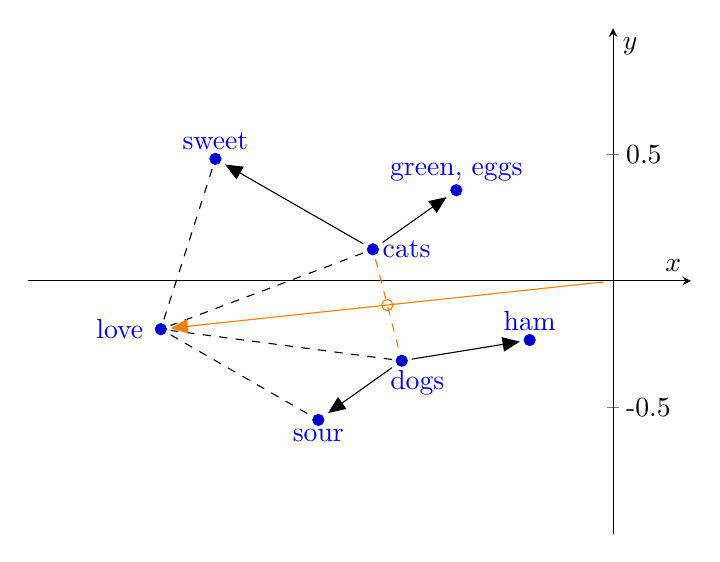
\begin{tikzpicture}
	\begin{axis}[axis lines=center,
		xmin=-0.75,xmax=0.1, ymin=-1,ymax=1,
		width=10cm,height=8cm,
		%xtick={-0.5},
		xtick={0},
		ytick={-0.5,0,0.5},
		%xticklabels={$\text{-}0.5$},
		yticklabels={$~\text{-}0.5$,$0$,$~0.5$},
		xlabel=$x$,ylabel=$y$,
		yticklabel style={right}]
		\addplot+[only marks,point meta=explicit symbolic, nodes near coords] coordinates 
		{
			(-0.308,  0.125)[]
			(-0.271, -0.316)[]
			(-0.201,  0.359)[green, eggs]
			(-0.107, -0.234)[ham]
			(-0.58 , -0.191)[]
			(-0.378, -0.55)[]
			(-0.51 ,  0.483)[sweet]
		};
	    \addplot+[only marks,point meta=explicit symbolic, nodes near coords,mark=o,mark options={color=orange,fill=orange}] coordinates
	    {
	    	(-0.2895,-0.0955)[]
	    };
	% Bisection line
	%\addplot+[domain=-0.75:0.2,sharp plot,mark=none,color=orange]{0.329*x};
	\node (origin) at (axis cs:0,0){};
	\node (cats) at (axis cs:-0.308,0.125){};
	\node[anchor=west,color=blue] (catsl) at (axis cs:-0.308,0.125){cats};
	\node (dogs) at (axis cs:-0.271,-0.316){};
	\node[anchor=north,color=blue] (dogsl) at (axis cs:-0.251,-0.316){dogs};
	\node (green) at (axis cs:-0.201,0.359){};
	\node (ham) at (axis cs:-0.107,-0.234){};
	\node (love) at (axis cs:-0.58,-0.191){};
	\node[anchor=east,color=blue] (lovel) at (axis cs:-0.59,-0.191){love};
	\node (sour) at (axis cs:-0.378,-0.55){};
	\node[anchor=north,color=blue] (sourl) at (axis cs:-0.378,-0.55){sour};
	\node (sweet) at (axis cs:-0.51, 0.483){};
	\draw[->](cats)--(green);
	\draw[->](cats)--(sweet);
	\draw[-,dashed](cats)--(love);
	\draw[-,dashed](love)--(sweet);
	\draw[-,dashed](dogs)--(love);
	\draw[-,dashed](love)--(sour);
	\draw[->](dogs)--(ham);
	\draw[->](dogs)--(sour);
	\draw[->,color=orange](origin)--(love);
	\draw[-,dashed,color=orange](cats)--(dogs);
\end{axis}
\end{tikzpicture}
\caption{A plot of the two-dimensional vectors generated for the 8 unique words in the Green Eggs and Ham corpus.}
\label{fig:eggs-plot}
\end{figure}

Since the spaces produced by these word embedding algorithms are vector spaces in a formal mathematical sense, we can use powerful tools from linear algebra to \textit{re-orient} our visualization from Figure \ref{fig:eggs-plot}, allowing us to build our intuition about various aspectsof the corpus' semantic relations. For example, looking at the original plot, we can observe that the $x$-axis neatly separates \textit{most} of the vectors into a cat quadrant (above the $x$-axis) and dog quadrant (below the $x$-axis), but that the arrangement is a bit skewed such that the vector for ``love'' lies within the dog quadrant, despite the fact that it actually perfectly bisects the angle formed by the ``cat'' and ``dog'' vectors (that is, the orange line in the figure passes through the midpoint of the dashed orange line joining ``cats'' and ``dogs'', the point labeled in the figure via an unfilled orange circle). Thus, as researchers, we may be able to get an even better sense of the dog vs. cat relation by \textit{rotating} the points clockwise until the vector for ``love'' is exactly aligned with the $x$-axis, as pictured in Figure \ref{fig:eggs-plot-rotated}.

%%% Eggs plot, rotated

\begin{figure}[ht!]
	\centering
	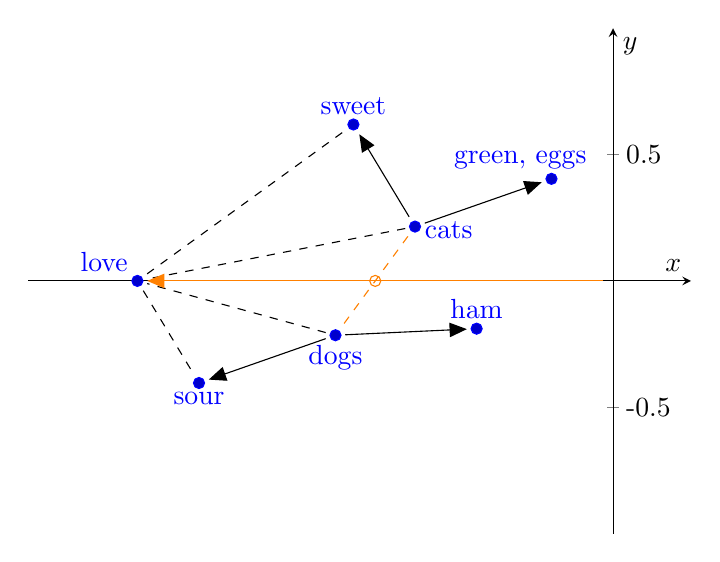
\begin{tikzpicture}
		\begin{axis}[axis lines=center,
			xmin=-0.75,xmax=0.1, ymin=-1,ymax=1,
			width=10cm,height=8cm,
			%xtick={-1.0},
			xtick={0},
			ytick={-0.5,0,0.5},
			%xticklabels={$\text{-}0.5$},
			yticklabels={$~\text{-}0.5$,$0$,$~0.5$},
			xlabel=$x$,ylabel=$y$,
			yticklabel style={right}]
			\addplot+[only marks,point meta=explicit symbolic, nodes near coords] coordinates 
			{
				(-0.254,0.215)[] % cats
				(-0.356,-0.215)[] % dogs
				(-0.079,0.404)[]
				(-0.175,-0.189)[ham]
				(-0.61,0.0)[] % love
				(-0.531,-0.404)[] % sour
				(-0.333,0.619)[sweet]
			};
			\addplot+[only marks,point meta=explicit symbolic, nodes near coords,mark=o,mark options={color=orange,fill=orange}] coordinates
			{
				(-0.305,0.0)[]
			};
			% Bisection line
			%\addplot+[domain=-0.75:0.2,sharp plot,mark=none,color=orange]{0.329*x};
			\node (origin) at (axis cs:0,0){};
			\node (cats) at (axis cs:-0.254,0.215){};
			\node[anchor=west,color=blue] (catsl) at (axis cs:-0.254,0.20){cats};
			\node (dogs) at (axis cs:-0.356,-0.215){};
			\node[anchor=north,color=blue] (dogsl) at (axis cs:-0.356,-0.215){dogs};
			\node (green) at (axis cs:-0.079,0.404){};
			\node[anchor=south,color=blue] (greenl) at (axis cs:-0.119,0.404){green, eggs};
			\node (ham) at (axis cs:-0.175,-0.189){};
			\node (love) at (axis cs:-0.61,0.0){};
			\node[anchor=east,color=blue] (lovel) at (axis cs:-0.61,0.075){love};
			\node (sour) at (axis cs:-0.531,-0.404){};
			\node[anchor=north,color=blue] (sourl) at (axis cs:-0.531,-0.404){sour};
			\node (sweet) at (axis cs:-0.333, 0.619){};
			\draw[->](cats)--(green);
			\draw[->](cats)--(sweet);
			\draw[-,dashed](cats)--(love);
			\draw[-,dashed](love)--(sweet);
			\draw[-,dashed](dogs)--(love);
			\draw[-,dashed](love)--(sour);
			\draw[->](dogs)--(ham);
			\draw[->](dogs)--(sour);
			\draw[->,color=orange](origin)--(love);
			\draw[-,dashed,color=orange](cats)--(dogs);
		\end{axis}
	\end{tikzpicture}
	\caption{The same points as in Figure \ref{fig:eggs-plot}, but rotated clockwise so that the ``love'' vector is aligned with the $x$-axis.}
	\label{fig:eggs-plot-rotated}
\end{figure}

By performing this rotation we thus obtain a clean separation which corresponds to our intuition with respect to the original corpus: words pertaining to cats in particular are in the cat quadrant (above the $x$-axis), those pertaining to dogs in particular are in the dog quadrant (below the $x$-axis), and the vector for the word ``love'', since it is neutral with respect to the cats-dogs split (i.e., since both cats and dogs are described as loving something), is  now located exactly on the boundary point between the quadrants. Although the pattern which emerges could have been seen (via a tilt of the head) in the original plot, this ability to re-orient the embedding space visualizations as needed becomes crucial for more complex corpora.

As another example of a useful re-orientation, consider the case of a researcher who studies the rotated plot in Figure \ref{fig:eggs-plot-rotated}, identifies the dog quadrant vs. cat quadrant pattern, and wants to explore this axis further. By employing another linear-algebraic transformation we can rotate and rescale the points so that the cats-to-dogs vector itself serves as our $x$-axis, allowing us to examine where the remaining points fall on this cats-to-dogs spectrum, as pictured in Figure \ref{fig:eggs-plot-orthogonal}. With this transformation, two salient splits now become evident: first, the cat and dog regions from before are now split (by construction) by the $y$-axis, with the cat region to its left and the dog region to its right. A second, new split can now be seen as well: that between food words (above the newly-constructed $x$-axis) and taste words (below the $x$-axis). The utility of this transformation is immediately apparent: with the four-quadrant separation resulting from the combination of these two splits (that is, starting from the upper-right quadrant and moving clockwise: dog-food words, dog-taste words, cat-taste words, and cat-food words), one could analyze a much more complex corpus by seeing how it ``sorts'' the words across the corpus into these categories. And indeed, computational linguist Dan Jurafsky performed just this sort of analysis on a much larger corpus---a collection of culinary descriptions from restaurant menus around the globe---as the basis for his award-winning book \textit{The Language of Food: A Linguist Reads the Menu} (\cite{jurafsky_language_2014}).

\begin{figure}[ht!]
	\centering
	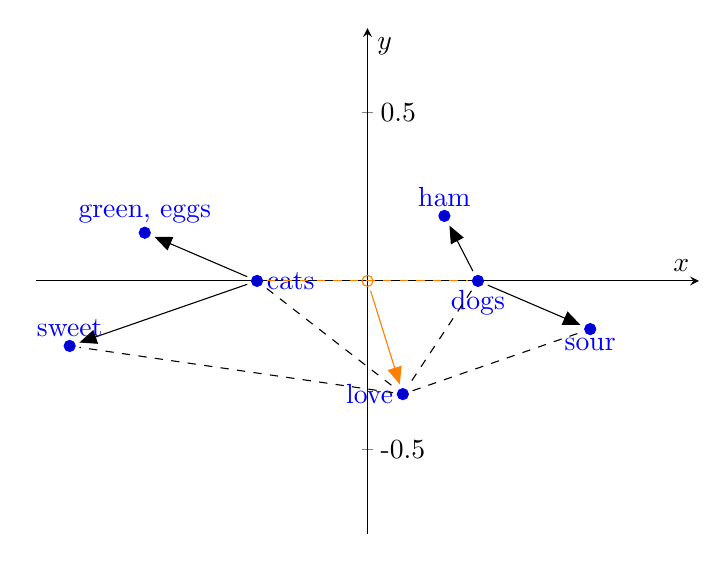
\begin{tikzpicture}
		\begin{axis}[axis lines=center,
			xmin=-1.5,xmax=1.5, ymin=-1.5,ymax=1.5,
			width=10cm,height=8cm,
			%xtick={-1.0},
			xtick={0},
			ytick={-1,0,1},
			%xticklabels={$\text{-}0.5$},
			yticklabels={$~\text{-}0.5$,$0$,$~0.5$},
			xlabel=$x$,ylabel=$y$,
			yticklabel style={right}]
			\addplot+[only marks,point meta=explicit symbolic, nodes near coords] coordinates 
			{
				(-0.500,0.000)[] % cats
				(0.500,0.000)[] % dogs
				(-1.008,0.286)[] % green, eggs
				(0.348,0.386)[ham]
				(0.160,-0.672)[] % love
				(1.008,-0.286)[] % sour
				(-1.348,-0.386)[sweet]
			};
			\addplot+[only marks,point meta=explicit symbolic, nodes near coords,mark=o,mark options={color=orange,fill=orange}] coordinates
			{
				(0.0,0.0)[]
			};
			% Bisection line
			%\addplot+[domain=-0.75:0.2,sharp plot,mark=none,color=orange]{0.329*x};
			\node (origin) at (axis cs:0,0){};
			\node (cats) at (axis cs:-0.5,0.0){};
			\node[anchor=west,color=blue] (catsl) at (axis cs:-0.5,0.0){cats};
			\node (dogs) at (axis cs:0.5,0.0){};
			\node[anchor=north,color=blue] (dogsl) at (axis cs:0.5,0.0){dogs};
			\node (green) at (axis cs:-1.008,0.286){};
			\node[anchor=south,color=blue] (greenl) at (axis cs:-1.008,0.286){green, eggs};
			\node (ham) at (axis cs:0.348,0.386){};
			\node (love) at (axis cs:0.160,-0.672){};
			\node[anchor=east,color=blue] (lovel) at (axis cs:0.160,-0.672){love};
			\node (sour) at (axis cs:1.008,-0.286){};
			\node[anchor=north,color=blue] (sourl) at (axis cs:1.008,-0.286){sour};
			\node (sweet) at (axis cs:-1.348, -0.386){};
			\draw[->](cats)--(green);
			\draw[->](cats)--(sweet);
			\draw[-,dashed](cats)--(love);
			\draw[-,dashed](love)--(sweet);
			\draw[-,dashed](dogs)--(love);
			\draw[-,dashed](love)--(sour);
			\draw[->](dogs)--(ham);
			\draw[->](dogs)--(sour);
			\draw[->,color=orange](origin)--(love);
			\draw[-,dashed,color=orange](cats)--(dogs);
		\end{axis}
	\end{tikzpicture}
	\caption{The same points as in Figures \ref{fig:eggs-plot} and \ref{fig:eggs-plot-rotated}, but this time rotated and rescaled so that the vector from ``cats'' to ``dogs'' now serves as our $x$-axis.}
	\label{fig:eggs-plot-orthogonal}
\end{figure}

A key lesson can be drawn from this this example for the sake of studying political theory\footnote{Here we focus on political theory in general (i.e., viewed synchronically) rather than the history of political thought (viewed diachronically) since a genuinely historical study will require a model of how these embeddings evolve through \textit{time}, which we indeed develop starting in Section \ref{sec:methods-diachronic} below.}, namely, that the effectiveness of these embedding algorithms for capturing semantic relations in a text depends upon how \textit{systematically} the text employs key terms (i.e., whatever terms the researcher aims to study). That is, the algorithm's success in inferring meaningful semantic relations from just the four sentences in our constructed corpus was aided by the fact that the sentences straightforwardly delineated these semantic relations: each sentence contained a single subject-verb-object triad, with the subjects and objects shared across sentences, enabling the straightforward construction of the network structures visualized in Figures \ref{fig:eggs-plot} through \ref{fig:eggs-plot-orthogonal}.

With this in mind, then, the most direct analogue of our hypothetical example within political theory would thus be a political-theoretic text which similarly aims to systematically discuss key terms and their interrelationships. The obvious candidate in Western political thought would be Hobbes' \textit{Leviathan}, a text so self-consciously systematic that even a champion of contextualism like Skinner agrees with his Straussian critics in deeming it ``probably the most plausible candidate'' for ``a classic text which `makes eminent sense on its own'{}'' (\cite{tully_meaning_1988}, p. 104, quoting \cite{parekh_history_1973}, p. 173)\footnote{The strength of the claim can be seen even more clearly by considering the full passage from which the quoted snippet is taken: ``unlike [Paine's \textit{Agrarian Justice} or Burke's \textit{Reflections}], \textit{Leviathan} makes eminent sense on its own, [...] circumscribed but not limited by its own historical conditions.'' (\cite{parekh_history_1973}, p. 173)}. \textit{Leviathan} stands out from other texts, that is, in Hobbes' attempt to construct an entirely self-contained and internally-cohesive system of political terms, making minimal reference (polemical or otherwise) to other texts\footnote{Hobbes' project in \textit{Leviathan} thus stands in stark contrast to e.g. Marx's in \textit{Critique of Hegel's `Philosophy of Right'} (discussed in the next chapter), which consists entirely of explicit references to excerpts from Hegel, or his \textit{Herr Vogt}, which is infused with dozens of implicit references in the form of puns and ironic statements which are unintelligible without knowledge of Vogt and his background.}.

Thus, in Figure \ref{fig:lev-embeddings}, we present a two-dimensional visualization of an embedding space constructed from the original English text of Hobbes' \textit{Leviathan}\footnote{An interesting comparative study---outside the scope of our demonstrative example, but pertaining directly to some of Skinner's arguments in \cite{skinner_hobbes_2008}---could be performed by training an embedding algorithm on both the original English and the later Latin edition of the text, to test whether any new vocabularic innovations were introduced by way of the latter.}. While perhaps not as cleanly-structured as the manually-constructed Green Eggs and Ham example, we \textit{do} observe the algorithm distinguishing important clusters of words: key terms constituting the religious aspects of the text are seen in the bottom-right corner (``christ'', ``holy'', ``lord''), while a set of relevant vocabularic dyads can be seen throughout the space (``obey'' and ``fear'', ``civill'' and ``law'', ``common-wealth'' and ``soveraign'', ``authority'' and ``power''). The algorithm's formation of these clusters is already encouraging, and perhaps surprising, given the fact that the standard applications of these word embedding algorithms in Computer Science typically train them on enormous datasets with billions of sentences\footnote{Google's LaBSE model for example, mentioned above, is trained on the \href{https://commoncrawl.org/}{CommonCrawl corpus}, which contains over 6.4 PB (PB stands for ``petabytes'', with one petabyte being equal to 1,000 gigabytes (GB)) of data. The text file for Leviathan is about 1 kilobye (KB), meaning that the algorithm was able to detect these types of semantic relations even in a corpus 6,400,000,000,000 (6.4 trillion) times smaller than the standard CommonCrawl corpus used to train this algorithm in industry settings.}. To understand how such a generated space could be used as a tool for historical, sociological, economic, or other social-scientific research, we now turn to a review of existing works which have made effective use of embeddings to study social-scientific phenomena. We emphasize throughout, however, some key limitations of these works which our approach---by utilizing a newer generation of explicitly \textit{context-sensitive} embedding algorithms---is able to overcome.

%The effect of adding slightly more data can be seen in Figure \ref{fig:hobbes-embeddings}, where a joint embedding space is generated for \textit{Leviathan}, \textit{Behemoth}, and \textit{De Cive}: 

%  embedding algorithms are awe can begin by observing that embedding algorithms will be able to capture  considering an ``easy'' case of a text

%%%%%
% Hobbes embeddings
%%%%%

\begin{figure}[ht!]
	\centering
	
	\begin{tikzpicture}
		\begin{axis}[axis lines=center,
			xmin=1, xmax=7,
			ymin=-10-0.4, ymax=10+0.4,
			xtick={1,7},ytick={-10,10},
			xlabel=$x$,ylabel=$y$,
			x label style={anchor=west},
			y label style={anchor=south},
			width=\textwidth
			]
			\addplot+[only marks,point meta=explicit symbolic, nodes near coords] coordinates
			{
(2.4045865535736084, 3.981800079345703)[\entpgf{authority}]
(4.982620716094971, -7.800631046295166)[\entpgf{christ}]
(2.9104197025299072, 5.7709784507751465)[\entpgf{civill}]
(4.146951675415039, 9.405494689941406)[\entpgf{common-wealth}]
(1.2487008571624756, -0.7207204103469849)[\entpgf{externall\_impediment}]
(2.110340118408203, 2.9968762397766113)[\entpgf{fear}]
(1.9348148107528687, 1.7129795551300049)[\entpgf{free}]
(3.3026037216186523, 8.032057762145996)[\entpgf{government}]
(5.239315032958984, -7.335639953613281)[\entpgf{holy}]
(3.3217368125915527, 7.348580837249756)[\entpgf{justice}]
(2.253394842147827, -2.1352388858795166)[\entpgf{king}]
(3.637099266052246, -5.454532623291016)[\entpgf{kingdome}]
(3.0478007793426514, 5.627185344696045)[\entpgf{law}]
(3.6457087993621826, 8.718162536621094)[\entpgf{liberty}]
(6.149326324462891, -9.386823654174805)[\entpgf{lord}]
(2.0016136169433594, 2.2313578128814697)[\entpgf{obey}]
(2.6352310180664062, 4.666365146636963)[\entpgf{power}]
(4.0261406898498535, 8.316762924194336)[\entpgf{soveraign}]
    };
    \end{axis}
	\end{tikzpicture}

	\caption{Visualization of a 2D embedding space generated from the English text of Hobbes' \textit{Leviathan}.}
	\label{fig:lev-embeddings}
\end{figure}

Since the introduction of the first widely-used word embedding algorithm, \texttt{word2vec} (\cite{mikolov_distributed_2013}), in 2012, researchers in the social sciences have used these algorithms to incorporate information from textual corpora into studies which previously were restricted to using numeric or qualitative data. Recent studies have found, for example, that contextual embeddings are able to capture salient properties of social class \parencite{kozlowski_geometry_2019}, the ideology of political manifestos \parencite{rheault_word_2020}, and the influence of economics on legal decisions \parencite{ash_ideas_2017}. Of these three, the latter comes closest to our work, in attempting to study the linguistic properties captured by word embeddings using econometric methods for estimation of time-series effects.

A related literature, which predates the creation of word embedding algorithms, aims to quantitatively capture the existence, direction, and magnitude of ideological influence directly. \cite{barron_individuals_2018}, for example, studies ideological influence across a time series of French Revolutionary debate transcripts by introducing ``transience'' and ``novelty'' metrics, which quantify how much the content of a given text is adopted by future texts, and how much it differs from the content of earlier texts, respectively. Unlike the previously-mentioned studies, however, this literature has yet to explore the new possibilities opened up by the development of semantic embedding algorithms, instead opting for the more well-established approach of probabilistic topic modeling (described here in Appendix \ref{sec:pgms}).
%a set of older more established text-analysis methods known as Topic Models
%\footnote{Topic modeling algorithms such as Latent Dirichlet Allocation (LDA), the most widely-used method, utilize word collocation information to identify a set of $K$ semantic topics within a text corpus, where each topic is itself a probability distribution over words. When given a corpus of unlabeled New York Times articles, for example, these algorithms are able to identify a topic for which ``stock'', ``market'', and ``percent'' are the three highest-probability terms, another where ``restaurant'', ``sauce'', ``menu'' have highest probability, and so on \parencite{blei_topic_2013}. Thus, despite not having any information on what sections the articles were pulled from, the algorithm is able to group articles from the same section together with near-perfect accuracy.}.
Although these topic modeling algorithms are an effective tool for summarizing a corpus at a high level, they are ill-suited for the task of tracing out the trajectory of \textit{particular} terms or concepts over time. Since we are interested in how Marx was able to cement his particular set of terms as \textit{the} vocabulary for later socialist discourse, embeddings are uniquely effective in allowing us to look at exactly which contexts a given term was employed in by Marx, and how this differs from the term's typical contexts before and after Marx's intervention. In other words, while topic-modeling-based approaches can tell us \textit{that} Marx's writings influenced future socialist discourse, embedding-based approaches can tell us \textit{how} this influence operated -- which terms or concepts Marx utilized in particularly novel ways, and which of these illocutionary moves were and were not effective in terms of influencing subsequent socialist thought.

Studies across both of these literatures, moreover, have yet to adopt the contextual \textit{sentence} embeddings we use herein, which utilize a more recently-developed embedding method from 2019 known as \BERT{} \parencite{devlin_bert_2019}. \BERT{}, in essence, differs from previous embedding algorithms in that it generates \textit{joint} numeric representations for words \textit{and} the contexts in which they appear, rather than associating each word with a single embedding vector. This means that, e.g., the word ``\texttt{bank}'' within the sentence ``\texttt{I took my money to the bank.}'' would be given a different embedding from the same word within the sentence ``\texttt{I took a nap on the bank of the river.}''. With these context-differentiated vectors, then, we have a powerful computational tool for grappling with a key difficulty in linguistically-informed historical studies: the fact that ``words denote and are known to denote different things at the same time.'' (\cite{pocock_virtue_1985}, p. 30)

As visualized in Figure \ref{fig:bert-nobert}, this approach to polysemy changes the unit of analysis in our model: we are no longer modeling words themselves, but rather \textit{word-context pairs}. In this way, the context is \textit{explicitly integrated} into the numerical representations we use to understand an author's use of language, providing researchers with a quantitative implementation of precisely the type of Cambridge School-style contextual approach described above.
%The usefulness of this joint word-context modeling becomes apparent if we compare the two plots in Figure \ref{fig:bert-nobert}.


\begin{figure}[ht!]
	\centering
	\begin{tikzpicture}
		
		\begin{axis}[axis lines=center,
			%view={28}{22},
			xmin=0, xmax=1, ymin=0, ymax=1,
			%xtick={0,1},ytick={0,1.0},
			xlabel=$x$,ylabel=$y$,width=10cm,height=10cm]
			\addplot+[only marks,point meta=explicit symbolic, nodes near coords,black] coordinates 
			{
				% top left: withdrawal_drugs
				(0.2,0.79)[{\includesvg[width=5.5mm,height=5.5mm]{../figs/1F489.svg}}]
				(0.2,0.9)[$\textsf{withdrawal}_2$]
				(0.1,0.72)[$\textsf{addiction}$]
				(0.3,0.715)[$\textsf{drugs}$]
				% bottom left: bank_money
				(0.2,0.19)[{\includesvg[width=5.5mm,height=5.5mm]{../figs/1F4B0.svg}}]
				(0.2,0.3)[$\textsf{bank}_1$]
				(0.085,0.2)[$\textsf{money}$]
				(0.3,0.2)[$\textsf{teller}$]
				(0.2,0.1)[$\textsf{withdrawal}_1$]
				% top right: bank_water
				% waves
				%(0.8,0.8)[{\includesvg[width=5.5mm]{./ch0/figs/1F30A.svg}}]
				% droplet
				(0.8,0.79)[{\includesvg[width=5.5mm,height=5.5mm]{../figs/1F4A7.svg}}]
				(0.69,0.8)[$\textsf{bank}_2$]
				(0.8,0.9)[$\textsf{river}$]
				(0.8,0.71)[$\textsf{swim}$]
				(0.925,0.8)[$\textsf{stream}_1$]
				% bottom right: stream_music
				% 3 notes
				%(0.8,0.19)[{\includesvg[width=5.5mm,height=5.5mm]{./ch0/figs/1F3B6.svg}}]
				% 1 note
				(0.8,0.19)[{\includesvg[width=5.5mm,height=5.5mm]{../figs/1F3B5.svg}}]
				(0.8,0.3)[$\textsf{stream}_2$]
				(0.7,0.12)[$\textsf{revenue}$]
				(0.9,0.12)[$\textsf{music}$]
			};
			%\addplot+ graphics[xmin=0,xmax=96,ymin=0,ymax=96] {Dad64.png};
		\end{axis}
	\end{tikzpicture}
	\caption{A visualization of \BERT{}'s ability to compute numeric representations of the same word in multiple different contexts.}
	\label{fig:bert-nobert}
\end{figure}


This improvement upon the original set of word embedding algorithms is therefore crucial, we contend, for capturing the nuanced uses of language which occur frequently in political-ideological polemics---the same concern which originally motivated the Cambridge School shift from what an author is saying to what they are \textit{doing} with their words. Marx's 1860 polemic against Karl Vogt \parencite{marx_herr_1860}, for example, makes use of several puns and purposeful misspellings of the names of those he is attacking, thus evoking contexts which the reader would not otherwise have read into the ``standard'' usage of the words. For example, he calls a particular political opponent with the surname Ranigel ``Ran-Igel'', likening him to an ``Igel'', the German word for hedgehog---we would therefore want to keep Marx's use of ``Igel'' in this sense separate from uses of ``Igel'' in general German texts. In general, due to the harsh censorship of political writings under the regimes of Friedrich Wilhelm III and IV (1797--1840 and 1840--1861, respectively)\footnote{See \cite{rose_reading_1978} for a detailed treatment of the effects of this censorship on Marx's writings, and \cite{prawer_karl_1976} for a chronological examination of the explicit and implicit literary references in Marx's writings.}, pre-\BERT{} text-analysis methods which are unable to capture the wide variety of ironic, metaphorical, and figurative uses of words would thus be unable to capture many important political illocutions throughout 19th century German political discourse, which had to be performed almost exclusively by way of these figures of speech.

\subsection{Visualizing Contextual Fields}\label{sec:methods-visualizing}

While the embedding spaces we've seen thus far have, for expository purposes, been \textit{constructed} as two- or three-dimensional spaces, these toy models are insufficient in practice for analyzing the semantic content of a corpus. The rich variety of meanings which a set of words can be infused with---even within a single text, much less across a collection of texts in dialogue with one another---cannot be arranged neatly along two or three axes. For this reason, even the most bare-bones embedding algorithms typically aim to embed words and phrases within an extremely high-dimensional space: 300 dimensions in the original word2vec algorithm, for example, or 768 in the case of \BERT{}. 

The tradeoffs between lower- and higher-dimensional spaces can be seen by comparing the left and right sides of the decomposition equation shown in Figure \ref{fig:kozlowski-decomposition}. Each value in the right-side matrix must be estimated from the corpus information encoded in the left-side matrix. In the terminology of statistics, each additional term that must be estimated ``costs'' an additional \textit{degree of freedom}, which can be thought of as a measure of the ``richness'' of the information provided by the corpus. If the word ``alienation'' only appears in the corpus once or twice, for example, it will be difficult to generate a meaningful high-dimensional vector for this term, as this vector's semantic content is dependent upon (in fact, under the Firthian hypothesis, is \textit{defined by}) the \textit{range} of contexts in which the word is seen. In Figure \ref{fig:decomposition-bad}, for example, we can see that word 4 appears only one time in the corpus, in a single context (context 5) in which no other words appear. In this case, therefore, \BERT{} has no information about this word's relationship to any other word in the corpus, and thus no way to infer where its 768-dimensional vector (the fourth row in the Word Vectors matrix on the right-hand side of the equation, containing values $u_{4,1}$ through $u_{4,768}$) should be placed relative to the other word vectors in the generated space. In cases like these, we say that the dataset does not have a sufficient level of \textit{statistical power} for estimation of embeddings via this method\footnote{We note that this term is used \textit{in relation to} the method since, for example, the Word-Context matrix in Figure \ref{fig:decomposition-bad} \textit{could} have a sufficient level of statistical power for estimation of much smaller (say, two- or three-dimensional) word vectors.}.

\begin{figure}[ht!]
	\centering
	\[\arraycolsep=1.8pt\def\arraystretch{1.2}
	\begin{blockarray}{cccccc}
		\rot{\phantom{\textsf{\small{diiim 7689\,}}}} & \rot{\textsf{\small{context 1}}} & \rot{\textsf{\small{context 2}}} & \rot{\textsf{\small{context 3}}} & \rot{\textsf{\small{context 4}}} & \rot{\textsf{\small{context 5}}} \\
		\begin{block}{c[ccccc]}
			\textsf{word 1} & 0 & 7 & 1 & 2 & 0 \\
			\textsf{word 2} & 0 & 7 & 3 & 6 & 0 \\
			\textsf{word 3} & 0 & 6 & 4 & 0 & 0 \\
			\textsf{word 4} & 0 & 0 & 0 & 0 & 1 \\
			\textsf{word 5} & 7 & 4 & 1 & 0 & 0 \\[1.1ex]
		\end{block}
		& \BAmulticolumn{5}{c}{\small\text{Word-Context}} \\[-1.0ex]
		& \BAmulticolumn{5}{c}{\underbrace{\small{\text{\phantom{Word}Matrix\phantom{Word}}}}_{5 \times 5 \; = \; 25}} \\
	\end{blockarray}
	\approx
	\begin{blockarray}{ccccccccc}
		\rot{\textsf{\small{dim 1}}} & \rot{\textsf{\small{dim 2}}} & \rot{\textsf{\small{dim 3}}} & \rot{\textsf{\small{dim 4}}} & \rot{\textsf{\small{dim 5}}} & \rot{\textsf{\small{dim 6}}} & \cdots & \rot{\textsf{\small{dim 768}}} \\
		\begin{block}{[rrrrrrrrr]}
u_{1,1} & u_{1,2} & u_{1,3} & u_{1,4} & u_{1,5} & u_{1,6} & \cdots & u_{1,768} \\
u_{2,1} & u_{2,2} & u_{2,3} & u_{2,4} & u_{2,5} & u_{2,6} & \cdots & u_{2,768} \\
u_{3,1} & u_{3,2} & u_{3,3} & u_{3,4} & u_{3,5} & u_{3,6} & \cdots & u_{3,768} \\
u_{4,1} & u_{4,2} & u_{4,3} & u_{4,4} & u_{4,5} & u_{4,6} & \cdots & u_{4,768} \\
u_{5,1} & u_{5,2} & u_{5,3} & u_{5,4} & u_{5,5} & u_{5,6} & \cdots & u_{5,768} \\[1.1ex]
		\end{block}
		\BAmulticolumn{8}{c}{\underbrace{\small\text{\phantom{Word VectorsWo}Word Vectors\phantom{ Word VectorsWo}}}_{5 \times 768 \; = \; 3,840}} \\
	\end{blockarray}
	%\substack{{\textstyle\;\times\;}\\~\\~}
	\times \underbrace{V}_{768 \times 5}
	\]
	\caption{A case where the information about the corpus (the Word-Context Matrix on the left side) does not have sufficient statistical power to allow estimation of the word and context vectors (the matrices on the right side). At a high level, the algorithm is unlikely to be able to draw meaningful estimates for 7,680 parameters---the 3,840 entries in the word vectors matrix (the $u$ parameters), plus another 3,840 entries (not labeled) in the context vectors matrix $V$---using only 25 input data points. Looking more closely at the \textit{structure} of the input data, we also see that it has no information from which to infer word 4's context-sensitive relation to other words, as it appears in only one context which is not shared by any other word in the corpus.}
	\label{fig:decomposition-bad}
\end{figure}

For intuition regarding this tradeoff in language modeling, consider Quine's \textit{gavagai} thought experiment described above. If we have only one or two observations of a foreign-language speaker saying \textit{gavagai} while pointing at a running rabbit, we won't have a rich enough set of contexts for this term to be able to differentiate whether, e.g., it refers to the rabbit itself, to the rabbit's fur, to a running animal in general, to creatures with tails, the act of running itself, etc. With the few linguistic ``degrees of freedom'' available to us at this point, we can only at best infer some vague properties of the term---perhaps that it has to do with motion more so than stillness\footnote{Stretching the metaphor a bit for clarity: if our goal was to generate a mental word embedding space for the new language, after these few observations we could (at most) conservatively move the \textit{gavagai} point slightly closer to the point for \textit{motion} (or more accurately, given the inner workings of word embedding algorithms, the point(s) for terms which our model hypothesizes as highly likely to represent or relate to the concept of motion).}. As we observe the term being used more and more across a wider and wider range of contexts, however, we start accumulating enough ``linguistic degrees of freedom'' to allow us to more and more confidently and precisely map \textit{gavagai} within the broader linguistic field\footnote{In Section \ref{sec:methods-diachronic} below we will distinguish more precisely between linguistic \textit{utterances}---the particular instances where we've observed \textit{gavagai} being used---and the broader linguistic \textit{field} from which these utterances were constructed (the Saussurean \textit{parole} and \textit{langue}, respectively). For now it suffices to understand ``linguistic field'' as a working model of the foreign language which is built using data in the form of utterances of \textit{gavagai}.} of the foreign language.

Once we \textit{have} accumulated enough observations from the corpus to feel confident in our estimated embedding vectors, however, a second key question arises: how can we \textit{use} this high-dimensional embedding space to draw meaningful inferences about the language of different authors or across different timespans within our corpus? Turning to the high-dimensional vectors produced by the embedding algorithm, we may ask, what good are (e.g.) points in a 768-dimensional geometric space when humans can only visualize points in at most two or three dimensions? While we do have tools like the similarity metrics discussed in Section \ref{sec:methods-embeddings} above, in a sense these only provide hints as to the full landscape of the embedding space\footnote{To see this, consider e.g. the task of trying to reconstruct a subway map given only the distances between stations. As illustrated for the Swiss rail system in \cite{dokmanic_euclidean_2015}, even sophisticated algorithms can only produce an approximation of the underlying space (this process is nonetheless crucial for e.g. inferring 3D protein structures; see \cite{vendruscolo_recovery_1997})}. We can do better using a set of visualization algorithms created specifically to construct 2D and 3D representations of high-dimensional spaces.

The $t$-distributed Stochastic Neighbor Embedding ($t$-SNE) algorithm, for example, constructs a 2D (or 3D) plot with the goal of capturing the ``neighborhood structures'' present within a higher-dimensional space, identifying distinct clusters of points which are closer to one another than to the other points in the space. For intuition, one can imagine taking a point in 3D space $\alpha\text{\textsuperscript{\includesvg[scale=0.01]{../figs/Sphere.svg}}}$ and asking, if I construct a small sphere centered at this point and grow it larger and larger, how soon will it come into contact with another point in the 3D space $\beta\text{\textsuperscript{\includesvg[scale=0.01]{../figs/Sphere.svg}}}$? The $t$-SNE algorithm constructs corresponding points $\alpha^\circ$ and $\beta^\circ$ in \textit{2D} space such that, if I construct a small \textit{circle} centered at $\alpha^\circ$ and grow it larger and larger, a similar property will hold with respect to how long it takes for that circle to come into contact with $\beta^\circ$. In this way, nearby points in $N$-dimensional space remain nearby in the two-dimensional visualization.

A separate visualization tool called Principal Component Analysis (PCA) also constructs low-dimensional representations of high-dimensional spaces but, unlike $t$-SNE, focuses on capturing the \textit{variance} among points rather than their neighborhood structure. To this end PCA can be thought of simply as projecting all the points in the space down to two dimensions, from every possible angle, then choosing the most interesting of these projections with respect to how \textit{spread out} the points are. Thus, taking the scatterplot of points in Figure \ref{fig:pca-scatter} as an example, we can see in the figure what these points in 2D look like when projected down into one dimension, whether onto the $x$-axis (the short lines along the horizontal axis at the bottom) or the $y$-axis (the short lines along the vertical axis on the left).

\begin{figure}[ht!]
\centering
\includesvg[width=0.666\textwidth]{../figs/pca_scatter.svg}
\caption{100 randomly-generated points in 2D space, showing potential projections of these points down into one dimension on both the $x$ and $y$ axes (the short vertical and horizontal lines, respectively).}
\label{fig:pca-scatter}
\end{figure}

However, this figure also illustrates a potential drawback of these ``standard'' projections onto the $x$-axis or $y$-axis, namely, that they may not in fact be the most interesting projections with respect to capturing the directions along which the points vary most. If the points represented word embeddings learned from the WPA Slave Narrative Collection (\cite{yetman_background_1967}), for example, the reason for these points' diagonal arrangement is likely to be far more interesting to researchers than the points' original $(x,y)$ coordinates. Perhaps points closer to the bottom-left of the plot are those used in the context of describing masters, and those closer to the top-right are those used when describing fellow slaves, for example, while points closer to the top-left corner are more likely to refer to women than those closer to the bottom-right corner, regardless of their placement on the main diagonal.

The PCA algorithm captures this intuition, that the directions of highest \textit{variance} may be most salient to the researcher, by tossing out the original $(x,y)$ coordinate system and replacing it with a coordinate system based on Principal Components: the First Principal Component axis is the axis along which the data varies the most, while the Second Principal Component axis is the direction along which the data varies second-most. This process can be continued, in fact (e.g., to generate a 3D PCA plot), up to the $N$ dimensions of the original set of points, revealing its power as \textit{both} a dimensionality-reduction \textit{and} data-reorientation tool. In our working WPA Slave Narrative Collection example, for instance, our PCA plot has the same dimensionality (2D) as the original plot, but re-orients the points so that the $x$-axis is the axis of maximum variance and the $y$-axis that of second-highest variance, as illustrated in Figure \ref{fig:pca-scatter-transformed}.

\begin{figure}
\centering
\includesvg[width=0.666\textwidth]{../figs/pca_scatter_transformed.svg}
\caption{The same data as plotted in Figure \ref{fig:pca-scatter}, but transformed via PCA so that the horizontal axis represents the direction of greatest variance (the First Principal Component) while the vertical axis represents the direction of second-greatest variance (the Second Principal Component).}
\label{fig:pca-scatter-transformed}
\end{figure}

To see the usefulness of this method in practice, we start by computing two-dimensional word embeddings for terms in the WPA Slave Narratives corpus, obtaining the space illustrated in Figure \ref{fig:wpa-embeddings}. And indeed we see the type of non-$(x,y)$-oriented pattern that we hypothesized earlier: isolating key terms for race (``white'' and ``black'') and status within the slave system (``slave'' and ``master''), we can observe that a move from bottom-right to top-left corresponds to a move from ``black'' to ``slave'', and that a nearly identical move in the same direction brings us from ``white'' to ``master''. With this observation in mind, then, we can choose our own horizontal and vertical axes and then analyze other terms \textit{with respect to} this newly-meaningful left-right or up-down orientation. For example, we generate Figure \ref{fig:wpa-embeddings-transformed} with the same data but with the horizontal axis now representing the white-to-black orientation we observed in the original plot.

\begin{figure}[ht!]
	\centering
	
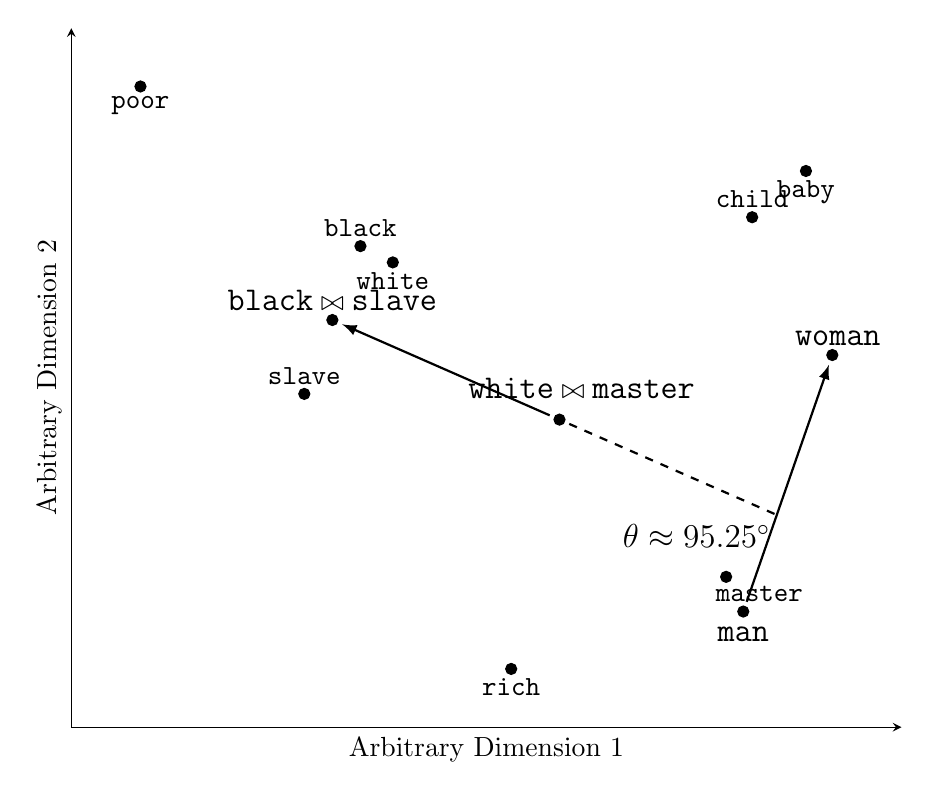
\begin{tikzpicture}
\pgfplotsset{ticks=none}
		\begin{axis}[
		    axis x line=bottom,
			axis y line=left,
			xmin=34.371693-1.7909069061279297, xmax=52.28076+1.7909069061279297,
			ymin=8.950363-1.1716894149780275, ymax=20.667257+1.1716894149780275,
			xtick={34.371693,52.28076},ytick={8.950363,20.667257},
			xlabel={Arbitrary Dimension 1},ylabel={Arbitrary Dimension 2},
			%x label style={anchor=west},
			%y label style={anchor=south},
			width=\textwidth
			]
			\addplot+[mark options={fill=black,color=black},only marks,point meta=explicit symbolic, nodes near coords] coordinates {
(49.975616455078125, 10.104655265808105)[]
(52.28076171875, 15.264684677124023)[]
(49.532535552978516, 10.802817344665527)[]
(40.06618118286133, 17.45557975769043)[]
(38.61276626586914, 14.48298168182373)[]
(40.904022216796875, 17.128196716308594)[]
(50.20615768432617, 18.036758422851562)[]
(51.59844207763672, 18.967124938964844)[]
(34.3716926574707, 20.66725730895996)[]
(43.968379974365234, 8.950363159179688)[]
(45.21827697753906, 13.965507507324219)[]
(39.339473724365234, 15.969280242919922)[]

};
\node (man) at (axis cs:49.975616, 10.104655){};
\node (woman) at (axis cs:52.28076, 15.264685){};
\node (master) at (axis cs:49.532536, 10.802817){};
\node (black) at (axis cs:40.06618, 17.45558){};
\node (slave) at (axis cs:38.612766, 14.482982){};
\node (white) at (axis cs:40.904022, 17.128197){};
\node (child) at (axis cs:50.206158, 18.036758){};
\node (baby) at (axis cs:51.598442, 18.967125){};
\node (poor) at (axis cs:34.371693, 20.667257){};
\node (rich) at (axis cs:43.96838, 8.950363){};
\node (whitemaster) at (axis cs:45.218277, 13.9655075){};
\node (blackslave) at (axis cs:39.339474, 15.96928){};
\node [inner sep=0] (intersect) at (axis cs:50.8438, 12.048069){};
\node[anchor = north, xshift=0.0, yshift=-2.0] (manl) at(axis cs: 49.975616, 10.104655){${\large \entpgf{man}}$};
\node[anchor = south, xshift=2.0, yshift=0.0] (womanl) at(axis cs: 52.28076, 15.264685){${\large \entpgf{woman}}$};
\node[anchor = north, xshift=12.0, yshift=0.0] (masterl) at(axis cs: 49.532536, 10.802817){$\entpgf{master}$};
\node[anchor = south, xshift=0.0, yshift=0.0] (blackl) at(axis cs: 40.06618, 17.45558){$\entpgf{black}$};
\node[anchor = south, xshift=0.0, yshift=0.0] (slavel) at(axis cs: 38.612766, 14.482982){$\entpgf{slave}$};
\node[anchor = north, xshift=0.0, yshift=0.0] (whitel) at(axis cs: 40.904022, 17.128197){$\entpgf{white}$};
\node[anchor = south, xshift=0.0, yshift=0.0] (childl) at(axis cs: 50.206158, 18.036758){$\entpgf{child}$};
\node[anchor = north, xshift=0.0, yshift=0.0] (babyl) at(axis cs: 51.598442, 18.967125){$\entpgf{baby}$};
\node[anchor = north, xshift=0.0, yshift=0.0] (poorl) at(axis cs: 34.371693, 20.667257){$\entpgf{poor}$};
\node[anchor = north, xshift=0.0, yshift=0.0] (richl) at(axis cs: 43.96838, 8.950363){$\entpgf{rich}$};
\node[anchor = south, xshift=8.0, yshift=4.0] (whitemasterl) at(axis cs: 45.218277, 13.9655075){${\large \entpgf{white} \bowtie \entpgf{master}}$};
\node[anchor = south, xshift=0.0, yshift=0.0] (blackslavel) at(axis cs: 39.339474, 15.96928){${\large \entpgf{black} \bowtie \entpgf{slave}}$};
\node[anchor = north, xshift=-29.0, yshift=0.0] (intersectl) at(axis cs: 50.8438, 12.048069){\large $\theta \approx 95.25^\circ$};
\draw[->,>=stealth,thick,,-latex](man) to (woman);
\draw[->,>=stealth,thick,,-latex](whitemaster) to (blackslave);
\draw[-,dashed,>=stealth,thick,](whitemaster) to (intersect);

\end{axis}
\end{tikzpicture}

	\caption{A two-dimensional embedding space trained on the WPA Slave Narratives corpus, where we draw solid arrows connecting points for key racial terms (``white'' and ``black'') and for terms denoting status within the slave system (``slave'' and ``master''), along with a dashed arrow connecting points for gendered terms (``man'' and ``woman'').}
	\label{fig:wpa-embeddings}
\end{figure}

\begin{figure}[ht!]
\centering
%\includesvg[width=\textwidth]{../figs/wpa_embeddings_transformed.svg}

\begin{tikzpicture}
\pgfplotsset{ticks=none}
		\begin{axis}[
			separate axis lines,
		    axis x line=bottom,
			axis y line=left,
			xmin=-1.0687146-0.3009931564331055, xmax=1.941217+0.3009931564331055,
			ymin=-1.0480828-0.21689443588256838, ymax=1.1208615+0.21689443588256838,
			xtick={-1.0687146,1.941217},ytick={-1.0480828,1.1208615},
			xlabel={$\entity{white} \bowtie \entity{master} \leftarrow$ Racial Slavery Dimension $\rightarrow \entity{black} \bowtie \entity{slave}$},ylabel={$\entity{man} \leftarrow$ Gender Dimension $\rightarrow \entity{woman}$},
			%x label style={anchor=west},
			%y label style={anchor=south},
			width=\textwidth
			]
			\addplot+[mark options={fill=black,color=black},only marks,point meta=explicit symbolic, nodes near coords] coordinates {
%(-0.9854497909545898, -0.42804527282714844)[]
%(-1.0687146186828613, 0.5719547271728516)[]
(-0.8816595077514648, -0.3472309112548828)[]
(0.9065628051757812, 0.04435586929321289)[]
(0.9736499786376953, -0.5407805442810059)[]
(0.7618718147277832, 0.05193376541137695)[]
(-0.6085567474365234, 0.8700709342956543)[]
(-0.7724103927612305, 1.120861530303955)[]
(1.9412169456481934, 0.1522383689880371)[]
(-0.12992000579833984, -1.0480828285217285)[]
%(-0.05989360809326172, -0.14764881134033203)[]
%(0.9401063919067383, -0.24821233749389648)[]

};
\node (master) at (axis cs:-0.8816595077514648, -0.3472309112548828){};
\node (black) at (axis cs:0.9065628051757812, 0.04435586929321289){};
\node (slave) at (axis cs:0.9736499786376953, -0.5407805442810059){};
\node (white) at (axis cs:0.7618718147277832, 0.05193376541137695){};
\node (child) at (axis cs:-0.6085567474365234, 0.8700709342956543){};
\node (baby) at (axis cs:-0.7724103927612305, 1.120861530303955){};
\node (poor) at (axis cs:1.9412169456481934, 0.1522383689880371){};
\node (rich) at (axis cs:-0.12992000579833984, -1.0480828285217285){};
\node (whitemaster) at (axis cs:-0.05989360809326172, -0.14764881134033203){};
\node (blackslave) at (axis cs:0.9401063919067383, -0.24821233749389648){};
\node [inner sep=0] (intersect) at (axis cs:-1.0168094635009766, -0.05141639709472656){};
\node[anchor = north, xshift=12.0, yshift=0.0] (masterl) at(axis cs: -0.8816595077514648, -0.3472309112548828){$\entpgf{master}$};
\node[anchor = south, xshift=0.0, yshift=0.0] (blackl) at(axis cs: 0.9065628051757812, 0.04435586929321289){$\entpgf{black}$};
\node[anchor = south, xshift=0.0, yshift=0.0] (slavel) at(axis cs: 0.9736499786376953, -0.5407805442810059){$\entpgf{slave}$};
\node[anchor = north, xshift=0.0, yshift=0.0] (whitel) at(axis cs: 0.7618718147277832, 0.05193376541137695){$\entpgf{white}$};
\node[anchor = south, xshift=0.0, yshift=0.0] (childl) at(axis cs: -0.6085567474365234, 0.8700709342956543){$\entpgf{child}$};
\node[anchor = north, xshift=0.0, yshift=0.0] (babyl) at(axis cs: -0.7724103927612305, 1.120861530303955){$\entpgf{baby}$};
\node[anchor = north, xshift=0.0, yshift=0.0] (poorl) at(axis cs: 1.9412169456481934, 0.1522383689880371){$\entpgf{poor}$};
\node[anchor = north, xshift=0.0, yshift=0.0] (richl) at(axis cs: -0.12992000579833984, -1.0480828285217285){$\entpgf{rich}$};

%\draw[ultra thin] (axis cs:\pgfkeysvalueof{/pgfplots/xmin},0) -- (axis cs:\pgfkeysvalueof{/pgfplots/xmax},0);
%\draw[ultra thin] (axis cs:0,\pgfkeysvalueof{/pgfplots/ymin}) -- (axis cs:0,\pgfkeysvalueof{/pgfplots/ymax});

\end{axis}
\end{tikzpicture}

\caption{The same points displayed in Figure \ref{fig:wpa-embeddings}, but transformed so that the horizontal axis represents the white-to-black direction within the space ($\entity{white} \bowtie \entity{master}$ on the left, $\entity{black} \bowtie \entity{slave}$ on the right), and the vertical represents the man-to-woman direction (\entity{man} below, \entity{woman} above).}
\label{fig:wpa-embeddings-transformed}
\end{figure}

Interestingly, after performing this translation, we can observe a second emergent feature of the word vectors' orientation: although in the original plot the move from ``woman'' to ``man'' seemed to be broadly similar to the move from ``white'' to ``master'' or ``black'' to ``slave'', once we differentiate the latter pairs by choosing them to be the horizontal and vertical axes (respectively), we can see that in fact the ``woman'' to ``man'' direction is \textit{diagonal} with respect to this new orientation---as we observed in our theoretical example above, this indicates that perhaps our analysis could benefit even more from setting the vertical axis to represent gender, as illustrated in Figure \ref{fig:wpa-embeddings-gender}.

%\begin{figure}[ht!]
%\centering
%\includesvg[width=\textwidth]{../figs/wpa_embeddings_gender.svg}
%\caption{The same embedding space as in Figures \ref{fig:wpa-embeddings} and \ref{fig:wpa-embeddings-transformed}, with the vertical axis now transformed to represent the man-to-woman direction, and with additional key terms plotted to enable analysis of their interrelationships with respect to these two sociologically-meaningful dimensions.}
%\label{fig:wpa-embeddings-gender}
%\end{figure}

The arbitrariness of the $(x,y)$ coordinates, and thus the impetus for employing PCA as one possibility for deriving \textit{meaningful} coordinates instead, is important enough to re-emphasize here: since the word embedding algorithms don't know the particular types of meaning we hope to capture, the coordinates generated for each word have no \textit{a priori} human-interpretable meaning at all; they are chosen solely on the basis of placing words closer together or further apart based on the similarity or difference between the contexts they appear in. In a 2D space, for example, if \textit{gavagai}'s initial embedding (typically randomly-chosen) lies directly below that of \textit{bird} and directly above that of \textit{fish}, but the algorithm observes \textit{gavagai} being used in a context which shows it is neither of these animals, the only way to increase its distance from \textit{both} points is to move \textit{gavagai}'s embedding left or right, i.e., to modify its $y$ coordinate. Since the same logic holds in cases where the three points randomly start out e.g. in a horizontal line (\textit{gavagai}'s embedding would have to be moved up or down), or on the $x$-$y$ diagonal (its embedding would have to be moved along the off-diagonal), we can see that the coordinates themselves have no stable or human-interpretable meaning on their own. It is up to the researcher to choose---on the basis of their research goals and/or intuitions regarding their field of study---how to transform the data to make sense of the embedding algorithm's outputs. Thus we have another example of how, as emphasized above, these algorithms do not \textit{automate} social-scientific research, but \textit{do} provide a powerful addition to the researcher's toolbox, to be used in conjunction with their own domain knowledge and expertise.

There is an unexplored dimension of the WPA embedding examples thus far, however, which may be crucial for a researcher's understanding of the corpus, especially in the social sciences and humanities. Namely: the spaces we've generated to this point have produced a \textit{single} point for each word, by \textit{averaging} its uses in various contexts over \textit{all} the interview subjects, when in reality what social science researchers often care about is precisely how the uses of these words \textit{differ} between different individuals or groups. If a researcher is analyzing the WPA Narratives with the goal of understanding 19th and early 20th century notions of freedom in the U.S., for example, it would be crucial to differentiate between how the term was used by slaves themselves versus how it was used by masters or overseers, just as historians have analyzed how (e.g.) John C. Calhoun and Frederick Douglass infused terms like ``liberty'' and ``freedom'' with very different semantic contents.

To this end, in the next section we describe a set of algorithms developed specifically to model not only the different \textit{senses} in which a word is used (which we saw above in our explanation of the \BERT{} algorithm), but also how different \textit{authors} emphasize or de-emphasize these senses. This brings us one step closer to our goal of understanding the history of political thought as a history of illocutionary moves since, as we argue, these author-specific emphases and de-emphases can be seen as textual manifestations of their attempts to \textit{steer} discourse in a certain direction: to steer popular understandings of ``liberty'' towards what we would today call ``negative liberty'' (freedom as non-interference) in Hobbes' case, for example, or to steer socialist discourse away from utopian ideals and towards political-economic categories, in Marx's.
%only that they should place points in such a way  which were, after all, based on arbitrarily chosen  axes along which the algorithm could move embedding points as their contexts were observed).

%Drawing on the examples of \cite{kozlowski_geometry_2019}, for example, bottom-leftmost point might be the embedding for the word ``man'', and the upper-rightmost point the embedding for ``woman''. In this case, for (e.g.) sociological research purposes, the original $x$ and $y$ coordinates of the points are not as interesting as their placement with respect to a line spanning from the ``man'' point to the ``woman'' point. Thus, 

\subsection{Author-Specific Embedding Spaces}\label{sec:auth-embeddings}

As we gestured towards at the end of the previous section, in order to further pinpoint the pathways through which political thought has evolved we'll need a model which can  keep track not only of the different \textit{senses} in which key terms are used, but also of the particular \textit{individuals} who use these terms in certain ways which shift their usage going forward. A recently-developed extension of the original \BERT{} algorithm \parencite{welch_exploring_2020} provides us with exactly the tool we need in this case, in explicitly constructing an additional personalized embedding for each (word, author) \textit{pairing} on top of the main contextual embedding for each word irrespective of author (i.e., relative to the entire corpus). This enables us to capture not only the shared terms and figures of speech available to all authors within a discursive community, but also the \textit{particular} ways in which they are employed---or wielded---by individual authors. Indeed, if one accepts (as we do) Skinner's contention that historians ought to treat these terms and figures of speech ``less as statements about the world than as tools and weapons of ideological debate'' (\cite{skinner_visions_2012}, p. 177), these author-specific embeddings provide a crucial tool for explicitly modeling how particular word-weapons were wielded by particular actors in particular wars of ideas, such as the battles for hegemony over socialist discourse that we analyze in future chapters.

%\jj{Skinner quote here about people operating by using the shared terms and figs of speech available}


\begin{figure}[ht!]
	\centering
	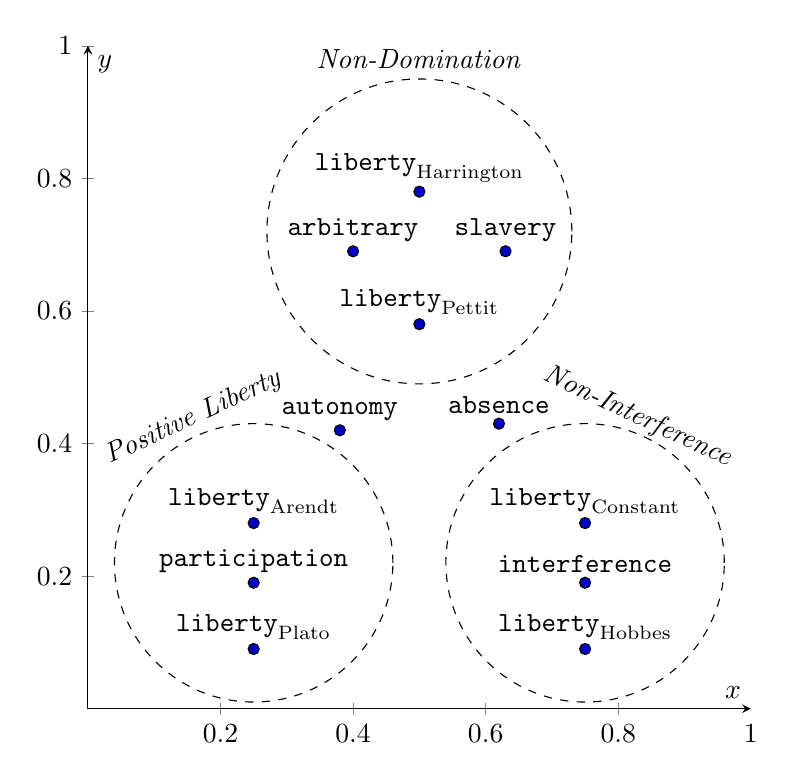
\begin{tikzpicture}
		\begin{axis}[axis lines=center,
			%view={28}{22},
			xmin=0, xmax=1, ymin=0, ymax=1,
			%xtick={0,1},ytick={0,1.0},
			xlabel=$x$,ylabel=$y$,width=10cm,height=10cm]
			\addplot+[only marks,point meta=explicit symbolic, nodes near coords,black] coordinates 
			{
				% top left: withdrawal_drugs
				(0.5,0.78)[$\texttt{liberty}_\text{Harrington}$]
				(0.5,0.58)[$\texttt{liberty}_\text{Pettit}$]
				(0.4,0.69)[$\texttt{arbitrary}$]
				(0.63,0.69)[$\texttt{slavery}$]
				% bottom left: bank_money
				(0.25,0.28)[$\texttt{liberty}_\text{Arendt}$]
				(0.25,0.09)[$\texttt{liberty}_\text{Plato}$]
				(0.25,0.19)[$\texttt{participation}$]
				(0.38,0.42)[$\texttt{autonomy}$]
				% top right: bank_water
				% waves
				%(0.8,0.8)[{\includesvg[width=5.5mm]{./ch0/figs/1F30A.svg}}]
				% droplet
				(0.62,0.43)[$\texttt{absence}$]
				(0.75,0.28)[$\texttt{liberty}_\text{Constant}$]
				(0.75,0.09)[$\texttt{liberty}_\text{Hobbes}$]
				(0.75,0.19)[$\texttt{interference}$]
				% bottom right: stream_music
				% 3 notes
				%(0.8,0.19)[{\includesvg[width=5.5mm,height=5.5mm]{./ch0/figs/1F3B6.svg}}]
				% 1 note
				%(0.8,0.3)[$\textsf{stream}_2$]
			};
			%\addplot+ graphics[xmin=0,xmax=96,ymin=0,ymax=96] {Dad64.png};
			% Positive Liberty + Circle
			\node[rotate=25] (a) at (axis cs:0.16,0.44) {\textit{Positive Liberty}};
			\draw[dashed] (axis cs:0.25,0.22) circle [blue, radius=0.21];
			\node[rotate=-25] (a) at (axis cs:0.83,0.44) {\textit{Non-Interference}};
			\draw[dashed] (axis cs:0.75,0.22) circle [blue, radius=0.21];
			% Non-Domination + Circle
			\node[] (a) at (axis cs:0.5,0.98) {\textit{Non-Domination}};
			\draw[dashed] (axis cs:0.5,0.72) circle [blue, radius=0.23];
		\end{axis}
	\end{tikzpicture}
	\caption{A visualization of \BERT{}'s ability to model the different contexts (and thus, senses) in which words are used by different authors. In this case \texttt{interference} falls squarely within the negative liberty (liberty as non-interference) cluster, as a term central to distinguishing negative from other forms of liberty, whereas \texttt{absence} falls between two clusters as it can be employed in both republican (``absence of arbitrary power'') and negative-liberty (``absence of interference'') contexts.}
	\label{fig:bert-author}
\end{figure}


%Although the embedding methods described in Section \ref{intro:methods} allowed us to construct a \textit{single} ideological space within which we were able to compare Marx's writings with those of his posited influences, in this section we need a more advanced technique which will allow us to trace the differential usage of various terms both over time and across authors (or groups of authors). Thus, for the explorations in this section we utilize a newer method introduced in
%\cite{welch_exploring_2020}, %\cite{personalized_2018},
%that of ``personalized'' word embeddings. While still estimating an overall ideological space based on the entire corpus (labeled \texttt{MAIN} in the resulting dataset), this approach also allows us to label each text with an author, for whom a separate set of embedding vectors is estimated.

Importantly, this method does not generate a separate embedding \textit{space} for every author, since our entire goal is to be able to \textit{compare} different authors' vectors on some common scale\footnote{i.e., for authors $A$, $B$, and $C$, the distance $\Dist(\vv{w_A}, \vv{w_B})$ between $A$'s vector for some word $w$ and $B$'s vector for $w$ must be on the same scale as the distance $\Dist(\vv{w_A}, \vv{w_C})$ between $A$'s vector for $w$ and $C$'s vector for $w$, as well as the distance $\Dist(\vv{w_B}, \vv{w_C})$ between $B$'s vector for $w$ and $C$'s vector for $w$.}. Instead, in the author-specific \BERT{} estimation, each author's specific vector $\vv{w_i}$ for a given term $w$ is estimated as an \textit{offset} relative to the vector for $w$ in the \texttt{MAIN} vector space, $\vv{w_\texttt{MAIN}}$. Given a vector $\vv{w_{PE}}$ representing the centroid of political-economic discourse within the broader ideological vector space (estimated via a procedure we detail in the next section), for example, this allows us to instantly check whether an author $A$ tends to use a term $w$ in a more political-economic context than some other author $B$, by checking whether $\Dist(\vv{w_A},\vv{w_{PE}}) < \Dist(\vv{w_B},\vv{w_{PE}})$, or relative to the ``average'' usage of the term across the entire corpus, by checking whether $\Dist(\vv{w_A},\vv{w_{PE}}) < \Dist(\vv{w_\texttt{MAIN}},\vv{w_{PE}})$.

Thus, while studies like \cite{kozlowski_geometry_2019} are able to discover shifts in the overall discourse around social class during the 20th century, for example that different education-related terms tended to become more dichotomous along the upper-class/lower-class axis, this modification of \BERT{} would allow them to identify \textit{which authors in particular} were ahead of the curve, adopting the newer senses of education-related terms earlier than others. Although a fully-developed methodology for testing the \textit{causal} impact of these early-adopters on the broader discourse is outside the scope of this paper, we are still therefore able to identify a necessary condition for causal influence---temporal precedence---and thus develop plausible causal hypotheses based on which authors' embeddings precede the overall embeddings in terms of the movement of key terms along socially meaningful axes.

To this end, especially when we turn to \textit{diachronic} embeddings below, we keep in mind the notion of \textit{Granger Causality} between two time-evolving data series $X_t$ and $Y_t$: if the values of $X$ up to some time $t$ help predict future values of $Y$ ($Y_{t+1}, Y_{t+2}, \ldots$) better than one could predict them solely on the basis of past values of $Y$, $X$ is said to exert Granger causality on $Y$. Thus, for example, if we consider $X_{\leq 1848}$ to be data representing Marx's pre-1848 speech acts, $Y_{\leq 1848}$ to be data representing language use by socialists besides Marx before 1848, and $Y_{> 1848}$ to be data representing language use by socialists besides Marx \textit{after} 1848, we can say that Marx's speech acts exerted Granger causality on socialist discourse to the extent that knowing $X_{\leq 1848}$ helps us predict the post-1848 trajectory of socialist discourse better than we could using $Y_{\leq 1848}$ alone (i.e., pre-1848 socialist discourse excluding Marx). Abstracting away from the details, then, when historians of political thought make claims like ``one cannot understand the trajectory of post-1848 socialist thought without understanding Marx [or Hegel, or Babeuf, etc.]''\footnote{Sholomo Avineri's \textit{The Social and Political Thought of Karl Marx}, for example, introduces its discussion of August von Cieszkowski with the claim that ``one cannot fully grasp Marx without recourse to Cieszkowski.'' (\cite{avineri_social_1968}, p. 125)} they are (perhaps unknowingly) making claims of Granger causality\footnote{On the applicability of this concept in the social sciences see the short entry in \cite{lewis-beck_sage_2003}, p. 439, or the more in-depth discussion in \cite{hlavackova-schindler_assumption_2012}. Within the humanities as such we have been able to locate only one work, \cite{wevers_tracking_2020}, which explicitly focuses on this conception of causality.}.

While testing for this type of causality using these author-specific embeddings is therefore possible in theory, in practice the problem of moving from associational to causal analysis is typically overshadowed by an even more fundamental problem, related to our discussion of \textit{degrees of freedom} in Section \ref{sec:methods-visualizing} above. While in that section we discussed how the researcher must have enough text---with words ranging over a rich enough variety of contexts---to allow estimation of all $N$ entries within each word's $N$-dimensional vector, the problem becomes even more acute when estimating author-specific spaces. Now, if there are $M$ authors in the corpus, the researcher must have enough text from \textit{each author} to estimate all $N \times M$ entries across the $M$ vectors generated for each word, plus the additional $N$ entries in the $N$-dimensional ``main'' word vector. Methodologically, this is why the algorithm's developers chose to estimate the single $w_\texttt{MAIN}$ vector for each word, and then learn each author's specific word embeddings $w_a$ as an \textit{offset} of this \texttt{MAIN} vector: this allows the algorithm to first pool \textit{all} of the scarce information about $w$ across the entire corpus towards estimating $w_\texttt{MAIN}$, then to estimate the author-specific embedding $w_a$ on the basis of how many degrees of freedom remained (with respect to the word $w$) to ``spend'' on this additional estimation.

In practice this means that researchers must take care when interpreting cases where an author's embedding $w_a$ for some key word $w$ seems not to differ much from $w_\texttt{MAIN}$. While ideally---that is, given enough textual data from each author---this indicates that the author's usage of $w$ indeed did not differ substantially from the general usage of $w$ across the corpus, it could also mean simply that the algorithm did not have enough data on this author to evaluate their usage, and thus ``guessed'' their usage to be at or near the corpus-average usage, for lack of any better way to choose. This latter case corresponds to the heuristic where, for example, if we only know that a man is Dutch, our best guess as to his height would be just the average height of Dutch men (182.5 cm, or about 6 ft.).

This analogy also points the way towards a potential modification of the approach, however, which we use to minimize the chances that this collapse-to-the-average affects our results. Within the analogy, note that if we could obtain additional salient information about this man, such as his membership within a \textit{subset} of the Dutch population, we could narrow the group over which we're taking the heuristic average. For example, if we learned that he was on the Dutch Olympic basketball team, we could do much better by guessing his height to be the average height of this team's members (about 6 ft. 7 in.), rather than that of the Dutch population as a whole. Thus in our case, to address this collapsing-to-the-average issue for authors with a small number of extant texts, we instead group individual authors into ``meta-authors'' based on the discursive community they are generally associated with in the historical literature---chosen to be as specific and/or exclusive as possible to minimize the distortions introduced by algorithmic averaging\footnote{Considering the Dutch basketball player example again, this matches our intuition that the average height of the Olympic team would provide a better guess than, for example, the average height of all Dutch basketball players or athletes in general, as the former represents a much smaller height-related subset of the population.}. Thus, for example, the texts of Bruno and Edgar Bauer, Arnold Ruge, Max Stirner, etc., are combined into one Young Hegelian meta-author in order to estimate a vector $\vv{w_{YH}}$ representing the centroid of Young Hegelian discourse (as defined by this author-to-group mapping) within the broader ideological space of 19th-century German discourse. Importantly, however, this approach is \textit{not} used to generate the political-economic and Hegelian vectors which serve as our orthogonal basis vectors, for reasons we describe in the next section.

\subsection{Discursive Fields as Embedding Clusters}\label{sec:embedding-clusters}

In the previous section we introduced two special vectors $\vv{w_{PE}}$ and $\vv{w_H}$, representing the centroids of political-economic and Hegelian discourse respectively, which we do \textit{not} compute via author-specific embedding estimation. Instead, to minimize the dependence (in the statistical sense) between our two basis vectors and the vectors like $\vv{w_{Marx}}$ for which we want to observe movement over time, we compute these basis vectors as centroids of word clusters which are derived independently via the \cTFIDF{} measure\footnote{\cTFIDF{} stands for the Class-Based Text-Frequency minus Inverse Document Frequency measure, formally defined via the formula
\begin{align*}
\textsf{cTFIDF}(w_i,c_j) = \textsf{cf}(w_i,c_j) \cdot \log\left(1 + \frac{\overline{N}}{\textsf{f}(w_i)}\right),
\end{align*}
where $w_i$ represents the $i$th word in the corpus, $c_j$ represents the $j$th class (grouping of documents), and $\overline{N}$ represents the average number of words per class. $\textsf{cf}(w_i, c_j)$ measures the number of times word $w_i$ appears across class $c_j$'s documents, while $\textsf{f}(w_i)$ measures the number of times $w_i$ appears across the entire corpus. In this section we provide intuition for how this formula is able to capture the uniqueness of a word $w_i$ to a class of documents $c_j$, relative to all other classes (which we collectively denote as $c_{-j}$).
}, which generates a ranking of all terms in the corpus on the basis of how ``unique'' they are to political-economic texts relative to Hegelian texts (and vice-versa, by taking the $N$ terms with lowest, rather than greatest, \cTFIDF{} scores).

The intuition we aim to capture with this measure is that a word $w_i$ is more ``unique'' to a class of documents $c_j$ to the extent that it appears frequently \textit{within} $c_j$'s documents, but \textit{infrequently} within the documents of other classes. In the corpus of nineteenth-century socialist texts we use in later chapters, for example, we may observe the German word \dett{das} appearing frequently in Marx's writings, but it is not \textit{unique} to Marx's writings, since it also appears frequently in the writings of the other authors in the corpus. In this case, \dett{das} has a high \textit{class frequency} value relative to the class $c_\textsf{Marx}$ representing the collection of Marx's writings (denoted $\textsf{cf}(\dett{das}, c_\textsf{Marx})$), but also a high \textit{corpus-wide} frequency value (denoted $\textsf{f}(\dett{das})$). However, if we consider the term \dett{Mehrwert} (surplus value) instead, the frequency with which this word appears in Marx's writings is much higher than the average frequency of this word across all nineteenth-century authors, so that $\textsf{cf}(\dett{Mehrwert}, c_\textsf{Marx})$ is high but $\textsf{f}(\dett{Mehrwert})$ is low. Thus, as a simple measure of uniqueness, we can simply consider the ratio of these two quantities:
\begin{align*}
\textsf{Uniqueness}(w_i,c_j) = \frac{\textsf{cf}(w_i,c_j)}{\textsf{f}(w_i)},
\end{align*}
so that
\begin{align*}
\textsf{Uniqueness}(\dett{das}, c_\textsf{Marx}) &= \frac{high}{high} \approx 1\text{, while} \\
\textsf{Uniqueness}(\dett{Mehrwert}, c_\textsf{Marx}) &= \frac{high}{low} > 1,
\end{align*}
matching our intuition regarding the uniqueness of a word to a particular author. Note that the formula also allows us to measure how \textit{rare} a word is for a particular author: if Marx uses the term \dett{Utopie} significantly \textit{less} often than the other authors in the corpus, we'll now have a value for $\textsf{cf}(\dett{Utopie}, c_\textsf{Marx})$ which is lower than $\textsf{f}(\dett{Utopie})$, giving us
\begin{align*}
\textsf{Uniqueness}(\dett{Utopie}, c_\textsf{Marx}) = \frac{low}{high} < 1,
\end{align*}
so that now we can qualitatively characterize an author's use of a word $w_i$ in three ways:
\begin{itemize}
	\item If $\textsf{Uniqueness}(w_i, c_a) < 1$, the word is used \textit{less} often by the author than its average usage across authors in the corpus
	\item If $\textsf{Uniqueness}(w_i, c_a) \approx 1$, the author uses the word $w_i$ at about the average rate it is used by all authors in the corpus, and
	\item If $\textsf{Uniqueness}(w_i, c_a) > 1$, the author uses the word $w_i$ \textit{more} often than its average usage across all authors in the corpus.
\end{itemize}
The formal \textsf{cTFIDF} formula, then, is simply this intuitive \textsf{Uniqueness} measure with one modification enabling it to better capture a key empirical property of ``natural'' (human) languages: namely, that word frequencies in these languages exhibit what's called a ``power law'' distribution. In a linguistic context, this ``law'' is really just an observed tendency, found in nearly all known human languages, for the frequency of words to be inversely proportional to their frequency \textit{rank} in the language. In other words, if the frequency of the most common word is $f_1$, the second most frequent word tends to occur 1/2 as often, the third most frequent word 1/3 as often, an so on, such that the frequency of the $n$th most frequent word can be written as $f_n = (1/n)\cdot f_1$.

In English for example, the most frequent word (``the'') occurs about $f_1 = 50,000$ times per million words, the second-most frequent (``be'') occurs about half as often ($f_2 = (1/2)f_1$), the third-most frequent (``and'') about one-third as often ($f_3 = (1/3)f_0$), and so on, with this pattern (of the $n$th most frequent word occurring 1/$n$ as often) continuing all the way down to the rarest words in the language. Given this tendency, then, the frequencies of words will exhibit massive (exponential) differences when comparing among high-frequency words, but tiny differences when comparing low-frequency words, as shown by the orange points in Figure \ref{fig:power-law}. In the case of our \textsf{Uniqueness} measure, however, we don't want the difference between (e.g.) the first and second most frequent words to count 100 times more than the difference between the 100th and 101st most frequent words. Thus, to prevent this linguistic property from skewing our measurements, we replace the denominator with its \textit{logarithm}, ensuring a more gradual decrease in the denominator's value as we measure uniqueness for less frequent terms, illustrated by the blue points in Figure \ref{fig:power-law}.

%, since $\log(1/n) = \log(1)-\log(n) = -\log(n)$ (so that $\log(f_n) = \log((1/n)f_0) = \log(f_0) - \log(n)$), motivating our logarithmic transformation of the denominator in the final \textsf{cTFIDF} formula.

%since word frequencies across large corpora tend to exhibit what's known as a ``power law'' distribution, we can take the logarithm of the denominator (the overall frequency of $w_i$ across the entire corpus) to obtain a smoother, more linear sequence of frequency values as we move from the most-frequent to the least-frequent terms in the corpus overall. 

%Zipf's Law is not a deterministic law \textit{per se}, but rather an extremely robust observation that seems to hold across a wide range of ``naturally-arising'' datasets. 

\begin{figure}[ht!]
\centering
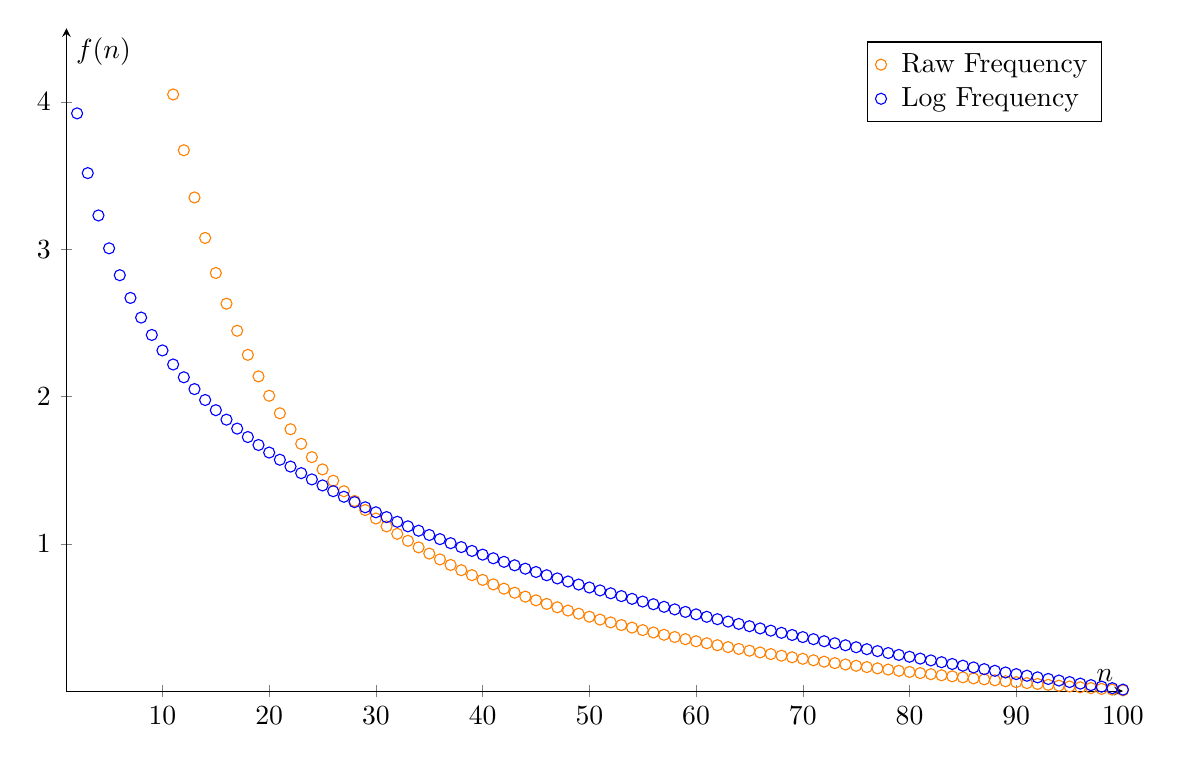
\begin{tikzpicture}
\begin{axis}[axis lines=center,
	xmin=1,
	%xmax=10000,
	ymin=0,ymax=4.5,
	width=15cm,height=10cm,
	%xtick={-0.5},
	%xtick={0},
	%ytick={-0.5,0,0.5},
	%xticklabels={$\text{-}0.5$},
	%yticklabels={$~\text{-}0.5$,$0$,$~0.5$},
	xlabel=$n$,
	ylabel=$f(n)$,
	xlabel style = {align=center},
	ylabel style = {align=center},
	legend cell align=left]
	%legend style={draw=none}
	%yticklabel style={right}]
\addplot+[domain=1:100,mark=o,only marks,color=orange,samples=100]{50*(1/x) - 50/101};
%\addlegendentry{$f(n) = 1/n$};
\addlegendentry{~Raw Frequency};
\addplot+[domain=1:100,mark=o,only marks,color=blue,samples=100]{ln(50*(1/x)) - ln(50/101)};
%\addlegendentry{$f(n) = \log(1/n)$};
\addlegendentry{~Log Frequency};
\end{axis}
%\begin{axis}[
%	scale only axis,
%	%xmin=-5,xmax=5,
%	axis y line*=right,
%	axis x line=none,
%	]
%\end{axis}
\end{tikzpicture}
\caption{An illustration of how the logarithm (plotted in blue) ``smoothes out'' the original corpus-wide frequencies (plotted in orange), where the horizontal axis represents a word's ranking in the corpus ($n=1$ representing the most frequent word, $n=2$ the second most frequent, and so on) and the vertical axis represents the frequencies of these words, measured in both original and logarithmic units. In particular, note that the logarithmic plot decreases the magnitude of the differences between the first \textasciitilde 30 words, and then slightly magnifies the differences between the remaining \textasciitilde 70 words, relative to the original frequency plot.}
\label{fig:power-law}
\end{figure}

%In particular, in Section \ref{sec:results} we will identify a movement in the language of 19th century socialist discourse writ large, away from philosophically-framed Hegelian terms and towards a more positivistic political-economic vocabulary, then identify Marx as a plausible cause of this shift due to the correlation between Marx's trajectory along this axis to the lagged trajectory of the corpus of 19th century socialist texts along the same axis.

With this modified, linguistic-theory-informed version of our \textsf{Uniqueness} measure in place we can to capture, in a mathematically- and linguistically-principled manner, the \textit{centrality} of certain terms to certain discursive genres: Hegelianism, political economy, Comtean positivism, etc. In future chapters we therefore use this approach to \textit{anchor} our axes, giving us a stable coordinate system---a common ruler---with which to measure differences in word usage between authors as well as changes in usage over time within and across these broadly-defined genres.

Specifically, the construction of these axes proceeds as follows: given a corpus $C$ containing words $\{w_1, w_2, \ldots, w_n\}$ and a set of genres $\{G_1, G_2, \ldots, G_m\}$ (where each genre is associated with a subset of the texts in the corpus which the researcher believes to be sufficiently representative of that genre), the researcher can compute ``genre-uniqueness scores'' $u_{i,j} = \textsf{cTFIDF}(w_i,G_j)$ for all (word, genre) pairings. With these scores in hand the researcher can then rank, for a chosen genre $G^*$, the $N$ words most unique to $G^*$ by choosing the $N$ words with the highest $\textsf{cTFIDF}(w_i,G^*)$ values. Once word embeddings for all words in the corpus have been generated, then, a \textit{centroid} vector representing the genre $G^*$ within this space can be computed as the \textit{weighted average} of the word vectors for the $N$ words found to be most unique to $G^*$. Once these centroid vectors have been computed, we can use them to orient ourselves within the otherwise arbitrary\footnote{Arbitrary, that is, with respect to the original $x$ and $y$ coordinates generated by the embedding algorithm.} geometric space. The movement of points through this space, for example, which before corresponded only to non-human-interpretable changes in the numeric values of a vector's 768 coordinates, can now be meaningfully interpreted with respect to one or more of these computed centroid vectors: a movement towards a centroid $G$ represents an increase in similarity to the semantics of this discursive genre, and vice-versa for a movement away from $G$. 

Social-scientifically, this interpretive lens enables us to analyze the linguistic field in terms of \textit{comparative statics}: holding some variables constant to enable the measurement of variation in others with respect to this static value. The ``Hegelian-ness'' of various authors in the corpus, for example, can be measured by comparing how their author-specific embedding vectors vary in relation to the static Hegelian genre-centroid vector. Or, we can evaluate an author's ``Hegelian-ness'' over time, by tracking changes in the distances between their author-specific vectors and the static Hegelian genre-centroid vector, over time.

This latter example, however, leaves some important questions unaddressed with respect to the nature of the linguistic fields we are studying: while treating a centroid for Hegel's writings as a constant in order to analyze changes in Marx may be reasonable, since these writings predated Marx's own (i.e., Hegel was not in interlocutory or back-and-forth dialogue with Marx in the same sense that Proudhon was), what do we do about the case where one author's speech acts feed into and have an effect on the very linguistic field from which another author subsequently draws when constructing their own speech acts? To incorporate \textit{time} as a variable in our analyses, we need to be able to model these complex linguistic feedback effects in a non-trivial way. That is, we need to explicitly augment our static embedding model with a model of the \textit{temporal relationships} between individual speech acts and the linguistic fields from which they are drawn.

As the first step in this direction, then, we begin the next section with an introduction to Saussurean structuralist linguistics. In particular, we discuss the distinction between \textit{langue} and \textit{parole} introduced by this approach, corresponding to the distinction between what we've been calling \textit{linguistic fields} and \textit{speech acts} thus far, and explain how this perspective gives rise to a working model of the \textit{mutual interactions} between these two co-constitutive phenomena which we can carry over into our computational approach.

%an author $a$'s discourse over time, for example, can be measured by seeing where their author-specific vectors for certain key terms are placed in the embedding space \textit{relative to} the Hegelian centroid vector. 


%with the use of a word like \dett{Sittlichkeit} (morality), for example, can be measured by seeing how close or far away the author-specific vector 

\subsection{Synchronic and Diachronic Analysis: Understanding the \textit{Langue}-\textit{Parole} Distinction}\label{sec:methods-diachronic}

Notwithstanding the progress in the field of semantic embeddings described at the end of Section \ref{sec:methods-ling-cambridge}, resulting in algorithms more and more capable of capturing meaning holistically across larger and larger linguistic units, there remain additional aspects of language---aspects crucial to social-scientific analysis---which we have not yet discussed and which will require a complementary set of tools to capture. To understand what the models thus far have lacked (and thus what additional tools we'll need to employ), however, we'll need to understand the Saussurean distinction between \textit{synchronic} and \textit{diachronic} approaches to language analysis.

%Understanding what aspects are and are not captured by the tools we've described up to this point, however, requires an understanding of 

Ferdinand de Saussure, in his \textit{Course on General Linguistics}, differentiates between two perspectives one can adopt when analyzing language: in the the first, which he calls the \textit{synchronic} perspective, the linguistic entities---texts, utterances, etc.---are treated as if they exist in a single moment in time (thus roughly corresponding to the notion of \textit{cross-sectional} analysis in the sciences), so that one can consider their interrelationships within a stable, static field of linguistic meaning. In other words, in the synchronic mode, one is concerned with understanding a particular collection of utterances, but \textit{not} with the dynamics by which these utterances, once issued, subsequently changed the field of language from which future utterances were generated (nor are they concerned with the other temporal direction: how past utterances shaped the linguistic field which gave rise to the utterances of interest). In Pocock's phrasing, however, the linguistic field that Cambridge School historians study is \textit{inherently}, definitionally diachronic, and must be studied in a diachronic mode:
\begin{quote}
``the diversity of linguistic contexts that went to determine what could be said but were at the same time acted upon by what was said.'' (\cite{pocock_virtue_1985}, p. 2)
\end{quote}

The models we've discussed thus far have all been essentially synchronic. The embedding algorithms, for example, are trained with the sole objective of capturing the relationships between \textit{words} and the \textit{contexts} they appear in across a given corpus, regardless of the temporal order in which the word-context pairs appeared. In reality, however, if we want our computational models to be able to aid in Cambridge School-style context-sensitive historical inquiry\footnote{That is to say, \textit{contextual} rather than textual analyses. If one was solely interested, for example, in evaluating the internal coherence of a single text like \textit{Leviathan}, the synchronic methods already introduced would be sufficient, as we saw in the \textit{Leviathan} embedding examples of Section \ref{sec:methods-embeddings}.}, we should take heed of the inherently diachronic emphasis of e.g. Pocock's definition cited above: ``a history of actors \textit{uttering and responding}''.

This Saussurean jargon may, at first glance, seem like a distinction without a difference: to obtain a diachronic model, one can simply train a sequence of synchronic models, one for each time period. We argue, however, that this misses the point of language modeling entirely: word embedding models are useful social-scientific tools because they implement a powerful theory of linguistic discourse---namely, the Firthian Hypothesis that we shall ``know a word by the company it keeps'' (\cite{firth_papers_1957}, p. 11)---which enables researchers to see (via the generated geometric spaces) the contours of how particular authors use particular words to do particular things. By the same logic, then, we argue that a diachronic language model is only useful or relevant for social-scientists to the extent that it can similarly implement an analytically-powerful theory of language change. Obtaining a sequence of trained word-embedding spaces is therefore necessary but \textit{not} sufficient for having a useful social-scientific tool. It must be paired with a theory regarding the \textit{relationship} between these time-slices, just as pairing the outputs of word embedding algorithms with the Firth Hypothesis provides us with a social-scientifically-grounded interpretive tool for understanding the relationship between words in the embedding spaces.

To this end, in the next section we survey the political-theoretic literature on the notion of \textit{influence}---an often-asserted but rarely-interrogated phenomenon in the practice of intellectual history---with an eye towards identifying what historians \textit{mean} when they posit that one event or thinker influenced another. Over the course of this survey, by pinning down this meaning as precisely as possible, we derive a coherent theory of influence which can thus serve as our lens through which to view and understand changes in embedding spaces over time.
%in the ideal speech situation of this modality, 
%utterances are not considered as \textit{responses} to other utterances but rather 

%Our discussion so far has focused on how computational methods can capture semantic meaning in a \textit{synchronic} mode: a term introduced by Saussure to refer to the notion of analyzing text as existing in a single moment in time.
%---with an eye towards illocutionary meaning---
%in text which we've assumed to be ``frozen in time'', i.e., without explicit reference 
%in that the models we've covered have been agnostic with respect to the temporal ordering of texts.

%To truly capture the types of meaning salient to political theorists, however, we must also have a model of the \textit{temporal relations} between texts.

%With this potential for computational text analysis in mind, in the next section we provide an overview of the early formation of Marx's political and economic thought, focusing on the key texts thought to have influenced Marx and how these influences manifested in his works.


\subsection{Putting it All Together: Networks of Semantic Influence}\label{sec:sln}

Although in previous sections we discussed how embedding spaces allow us to visualize the lexical-semantic relationships among individual terms, sentences, documents, and authors, the algorithms for constructing them operate only at the level of individual terms and sentences, such that information is lost when the resulting term or sentence embeddings are coarse-grained up to the document or authorial level. While we are many years away from embedding algorithms that can directly incorporate and model semantics above the sentence level\footnote{Even contextual sentence-level embedding algorithms are still in their infancy: while word embeddings have been in wide use since 2014 (after \cite{mikolov_distributed_2013}, the canonical citation for word embedding-based works, showed their immense effectiveness on a wide range of NLP tasks), with libraries for their construction available in nearly all programming languages by 2016, the first contextual sentence-level embedding library was not made available until 2020 (a year after the canonical publication, \cite{reimers_sentencebert_2019}), and at the time of writing no libraries are available for languages besides Python.}, we are able build on recent work in cultural analytics which combines the lexical-semantic modeling power of embeddings with explicit models of authorial influence, allowing us to perform more sophisticated author-level comparisons than would be possible through (e.g.) comparison of mean-pooled sentence embeddings.

In particular, we adopt the approach described in \cite{soni_abolitionist_2021} to construct a set of Semantic Leadership Networks which directly model dyadic-temporal influence among major sources of nineteenth-century European socialist thought. For example, to analyze the impact of pre-1848 socialist thought on that of the post-1848 era, we can consider the network in Figure \ref{fig:sln1}, where each edge represents the hypothesized lexical-semantic influence of one node before 1848 on the other after 1848.

\begin{figure}[ht!]
	\centering
	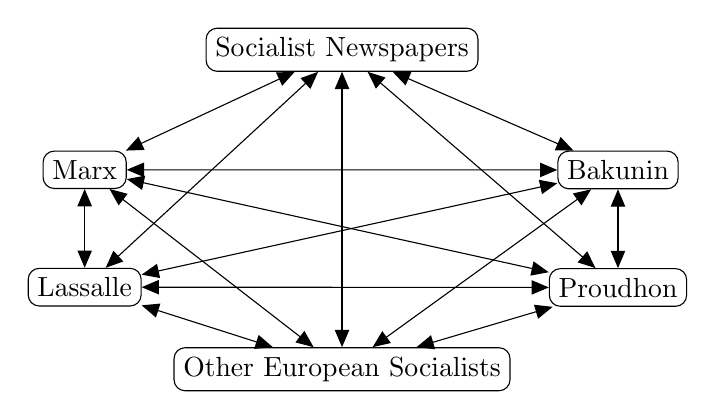
\begin{tikzpicture} %
		% Center
		\node[draw, rounded corners] (News) {Socialist Newspapers} ;
		\node[draw, below left=of News, rounded corners] (Marx) {Marx} ; %
		\node[draw, below right=of News, minimum width=8.5mm, rounded corners] (Bakunin) {Bakunin} ; %
		% Left
		\node[draw, below=of Marx, rounded corners] (Lassalle) {Lassalle} ;
		\node[draw, below=of Bakunin, rounded corners] (Proudhon) {Proudhon} ;
		%\node[right=of atp1] (atp2) {$\ldots$} ;
		% Fake nodes for getting the spacing right
		\node[below=of News] (Blank1) {} ;
		\node[below=of Blank1] (Blank2) {} ;
		\node[draw, below=of Blank2, rounded corners] (EuroSoc) {Other European Socialists} ;
		\edge [<->] {Marx} {Bakunin} ;
		\edge [<->] {Marx} {Lassalle} ;
		\edge [<->] {Marx} {Proudhon} ;
		\edge [<->] {Marx} {News} ;
		\edge [<->] {Marx} {EuroSoc} ;
		\edge [<->] {Bakunin} {Lassalle} ;
		\edge [<->] {Bakunin} {Proudhon} ;
		\edge [<->] {Bakunin} {News} ;
		\edge [<->] {Bakunin} {EuroSoc} ;
		\edge [<->] {Lassalle} {Proudhon} ;
		\edge [<->] {Lassalle} {News} ;
		\edge [<->] {Lassalle} {EuroSoc} ;
		\edge [<->] {Proudhon} {News} ;
		\edge [<->] {Proudhon} {EuroSoc} ;
		\edge [<->] {News} {EuroSoc} ;
	\end{tikzpicture}
	\caption{A PGM where we've observed the person's action ($a = \textsf{Go}$) but only have a probability distribution over the weather $w$.}
	\label{fig:sln1}
\end{figure}

Then to estimate the weights on these edges, i.e., the degree of lexical-semantic influence between a dyad of authors, we start by computing the ``lead'' of one author $a_1$ over another $a_2$ with respect to the movement of their respective embeddings for a particular word $w$ via the following equation, a simplified version of equation (4) from \cite{soni_abolitionist_2021}:
\begin{align*}
	\mathsf{Lead}_{a_1 \rightarrow a_2}(w) = \frac{\mathbf{pre}_w^{a_1} \cdot \mathbf{post}_w^{a_2}}{\mathbf{pre}_w^{a_2} \cdot \mathbf{post}_w^{a_2}},
\end{align*}
where the numerator represents the similarity between $a_1$'s pre-1848 embedding for $w$ and $a_2$'s post-1848 embedding for $w$ (both normalized to be of length one, an assumption we relax for the following definitions), and the denominator represents the similarity between $a_2$'s pre- and post-1848 embeddings for $w$. In other words, considering our word similarity function $\mathsf{sim}(\cdot, \cdot)$ described in the previous section, we compute
\begin{align*}
	\mathsf{Lead}_{a_1 \rightarrow a_2}(w) = \frac{\mathsf{sim}(\mathbf{pre}_w^{a_1}, \mathbf{post}_w^{a_2})}{\mathsf{sim}(\mathbf{pre}_w^{a_2}, \mathbf{post}_w^{a_2})}.
\end{align*}
As outlined in more detail in \cite{soni_abolitionist_2021}, this quantity operationalizes our concept of author $a_1$'s influence on author $a_2$ over a given time span: it increases in proportion to how much $a_2$'s post-1848 usage of $w$ is ``pulled'' towards $a_1$'s pre-1848 usage. For example, Figure \ref{fig:onewayinfluence} visualizes a situation where $a_2$'s post-1848 usage of a word $w$ is drawn away from their pre-1848 usage and towards $a_1$'s pre-1848 usage: intuitively, this can be thought of as $a_2$ being ``convinced'' to use $w$ in the manner they observed $a_1$ using it, thus dropping their original pre-1848 conception of $w$ over time.

\begin{figure}[ht!]
	\centering
	%\includegraphics[width=0.666\textwidth]{./ch2/figs/one_way_influence.tikz}
	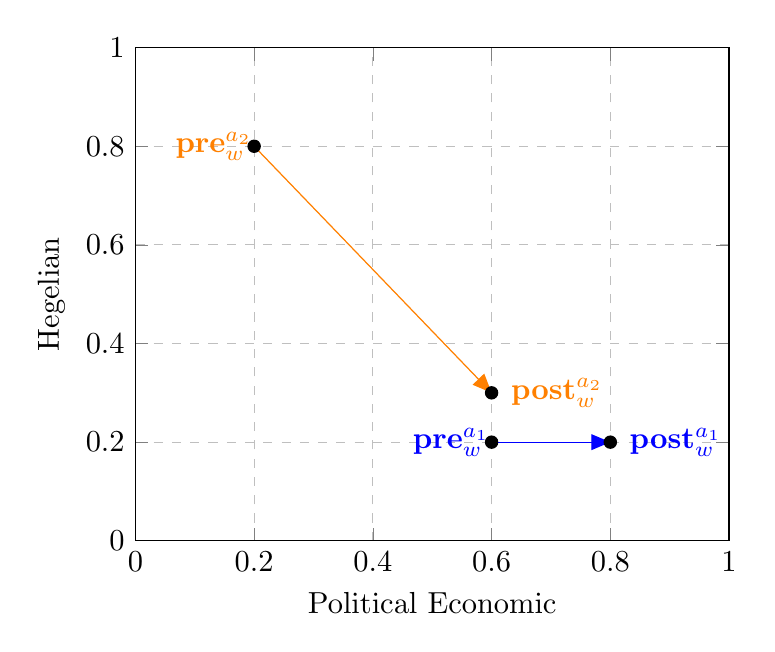
\begin{tikzpicture}[scale=1.1]
	\begin{axis}[
		%title={Temperature dependence of CuSO\(_4\cdot\)5H\(_2\)O solubility},
		xlabel={Political Economic},
		ylabel={Hegelian},
		xmin=0, xmax=1.0,
		ymin=0, ymax=1.0,
		xtick={0,0.2,0.4,0.6,0.8,1.0},
		ytick={0,0.2,0.4,0.6,0.8,1.0},
		legend pos=north west,
		ymajorgrids=true,
		xmajorgrids=true,
		grid style=dashed,
		]
		
		\addplot[
		color=blue,
		%mark=circle,
		->,
		smooth
		%patch,
		%mesh,% without mesh, pgfplots tries to fill
		%patch type=quadratic spline
		]
		coordinates {
			(0.6,0.2)(0.8,0.2)
		};
		%\legend{CuSO\(_4\cdot\)5H\(_2\)O}
		\addplot[
		color=orange,
		%mark=circle,
		->,
		smooth
		]
		coordinates {
			(0.2,0.8)(0.6,0.3)
		};
		
		\addplot[
		scatter/classes={a={blue}, b={orange}},
		%scatter/classes={%
			%	a={mark=square*,blue},%
			%	b={mark=triangle*,red},%
			%	c={mark=o,draw=black}},
		scatter, mark=*, only marks, 
		scatter src=explicit symbolic,
		nodes near coords*={\Label},
		nodes near coords style={
			%anchor=west,
			anchor=\perpointanchor,
			xshift=1mm,
			yshift=\perpointyshift,
			color=\perpointcolor
		},
		visualization depends on={value \thisrow{label} \as \Label},
		visualization depends on={value \thisrow{anchorclass} \as \perpointanchor},
		visualization depends on={value \thisrow{yshift} \as \perpointyshift},
		visualization depends on={value \thisrow{class} \as \perpointcolor}
		] table [meta=class] {
			x y anchorclass yshift class label
			0.6 0.2 east 0cm blue $\mathbf{pre}_w^{a_1}$
			0.8 0.2 west 0cm blue $\mathbf{post}_w^{a_1}$
			0.2 0.8 east 0cm orange $\mathbf{pre}_w^{a_2}$
			0.6 0.3 west 0cm orange $\mathbf{post}_w^{a_2}$
			%0.7 0.6 a C
			%0.35 0.4 a D
		};
		
	\end{axis}
\end{tikzpicture}

	\caption{The situation of one-way influence, where $\mathsf{Lead}_{a_1 \rightarrow a_2}(w) > \mathsf{Lead}_{a_2 \rightarrow a_1}(w)$, allowing us to infer that $a_1$'s usage of $w$ before 1848 had more influence on $a_2$'s usage over time than vice-versa.}
	\label{fig:onewayinfluence}
\end{figure}

Mathematically, assuming our embedding vectors are all in $\mathbb{R}^{[0,1]\times[0,1]}$, we can obtain a similarity metric $\Sim$ that scales from 0 to 1 via the transformation
\begin{align*}
	\Sim(\mathbf{v}_1, \mathbf{v}_2) = 1 - \frac{\|\mathbf{v}_2-\mathbf{v}_1\|}{\sqrt{2}},
\end{align*}
where $\|\mathbf{v}_2-\mathbf{v}_1\|$ represents the Euclidean distance between the embedding vectors $\mathbf{v}_1$ and $\mathbf{v}_2$, and where $\sqrt{2}$ represents the maximum Euclidean distance possible between two points in $\mathbb{R}^{[0,1]\times[0,1]}$. Then we can compute the Euclidean distances as:
\begin{align*}
	\|\postvec{w}{a_2} - \prevec{w}{a_1}\| &= \sqrt{(0.6-0.6)^2 + (0.3-0.2)^2} = \sqrt{0.1^2} = 0.1,\\
	\|\postvec{w}{a_2} - \prevec{w}{a_2}\| &= \sqrt{(0.6-0.2)^2 + (0.3-0.8)^2} = \sqrt{(0.4)^2 + (0.5)^2} = \sqrt{0.36} = 0.6,\\
	\|\postvec{w}{a_1} - \prevec{w}{a_2}\| &= \sqrt{(0.8-0.2)^2 + (0.2-0.8)^2} = \sqrt{0.6^2 + (-0.6)^2} = \sqrt{0.36 + 0.36} \\
	&= \sqrt{0.72} \approx 0.849,\\
	\|\postvec{w}{a_1} - \prevec{w}{a_1}\| &= \sqrt{(0.8-0.6)^2 + (0.2-0.2)^2} = \sqrt{0.2^2} = 0.2,
\end{align*}
and thus compute our leadership scores for this situation as:
\begin{align*}
	\Lead{a_1}{a_2}(w) &= \frac{\Sim(\prevec{w}{a_1}, \postvec{w}{a_2})}{\Sim(\prevec{w}{a_2}, \postvec{w}{a_2})} = \frac{1 - \frac{\|\postvec{w}{a_2} - \prevec{w}{a_1}\|}{\sqrt{2}}}{1 - \frac{\|\postvec{w}{a_2}-\prevec{w}{a_2}\|}{\sqrt{2}}} = \frac{1-\frac{0.1}{\sqrt{2}}}{1-\frac{0.6}{\sqrt{2}}} \approx \frac{0.929}{0.576} \approx 1.613,\\
	\Lead{a_2}{a_1}(w) &= \frac{\Sim(\prevec{w}{a_2}, \postvec{w}{a_1})}{\Sim(\prevec{w}{a_1}, \postvec{w}{a_1})} = \frac{1 - \frac{\|\postvec{w}{a_1} - \prevec{w}{a_2}\|}{\sqrt{2}}}{1 - \frac{\|\postvec{w}{a_1}-\prevec{w}{a_1}\|}{\sqrt{2}}} = \frac{1-\frac{0.849}{\sqrt{2}}}{1-\frac{0.2}{\sqrt{2}}} \approx \frac{0.340}{0.859} \approx 0.400,
\end{align*}
so that we obtain the result that $a_1$'s influence on $a_2$ in this case was about 4 times stronger than $a_2$'s influence on $a_1$.

Importantly, however, the $\mathsf{Lead}$ function also allows us to identify instances of \textit{mutual} influence between $a_1$ and $a_2$. In the most extreme case, visualized in Figure \ref{fig:mutualinfluence}, $a_1$'s usage of $w$ is influenced by $a_2$'s usage to such an extent that the former's post-1848 usage exactly matches the latter's pre-1848 usage and, with maximal influence also flowing from $a_1$ to $a_2$, $a_2$'s post-1848 usage exactly matches $a_1$'s pre-1848 usage. In other words, $a_1$ and $a_2$ have switched places---both authors drop their pre-1848 usage of $w$ and instead adopt the other author's usage.

\begin{figure}[ht!]
	\centering
	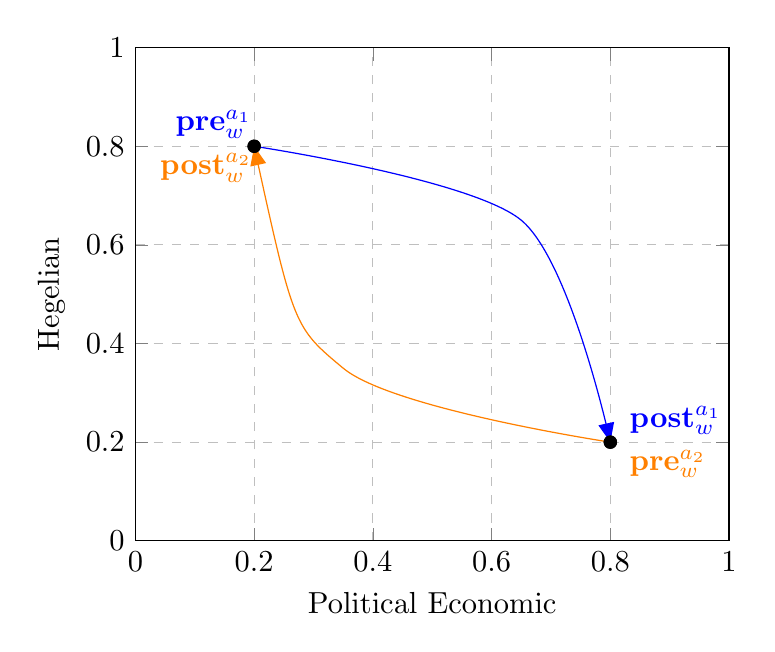
\begin{tikzpicture}[scale=1.1]
	\begin{axis}[
		%title={Temperature dependence of CuSO\(_4\cdot\)5H\(_2\)O solubility},
		xlabel={Political Economic},
		ylabel={Hegelian},
		xmin=0, xmax=1.0,
		ymin=0, ymax=1.0,
		xtick={0,0.2,0.4,0.6,0.8,1.0},
		ytick={0,0.2,0.4,0.6,0.8,1.0},
		legend pos=north west,
		ymajorgrids=true,
		xmajorgrids=true,
		grid style=dashed,
		]
		
		\addplot[
		color=blue,
		%mark=circle,
		->,
		smooth
		%patch,
		%mesh,% without mesh, pgfplots tries to fill
		%patch type=quadratic spline
		]
		coordinates {
			(0.2,0.8)(0.65,0.65)(0.8,0.2)
		};
		%\legend{CuSO\(_4\cdot\)5H\(_2\)O}
		\addplot[
		color=orange,
		%mark=circle,
		<-,
		smooth
		]
		coordinates {
			(0.2,0.8)(0.35,0.35)(0.8,0.2)
		};
		
		\addplot[
		scatter/classes={a={blue}, b={orange}},
		%scatter/classes={%
			%	a={mark=square*,blue},%
			%	b={mark=triangle*,red},%
			%	c={mark=o,draw=black}},
		scatter, mark=*, only marks, 
		scatter src=explicit symbolic,
		nodes near coords*={\Label},
		nodes near coords style={
			%anchor=west,
			anchor=\perpointanchor,
			xshift=1mm,
			yshift=\perpointyshift,
			color=\perpointcolor
		},
		visualization depends on={value \thisrow{label} \as \Label},
		visualization depends on={value \thisrow{anchorclass} \as \perpointanchor},
		visualization depends on={value \thisrow{yshift} \as \perpointyshift},
		visualization depends on={value \thisrow{class} \as \perpointcolor}
		] table [meta=class] {
			x y anchorclass yshift class label
			0.2 0.8 east 0.25cm blue $\mathbf{pre}_w^{a_1}$
			0.8 0.2 west 0.25cm blue $\mathbf{post}_w^{a_1}$
			0.2 0.8 east -0.25cm orange $\mathbf{post}_w^{a_2}$
			0.8 0.2 west -0.25cm orange $\mathbf{pre}_w^{a_2}$
			%0.7 0.6 a C
			%0.35 0.4 a D
		};
		
	\end{axis}
\end{tikzpicture}

	\caption{The situation of mutual influence, where $\mathsf{Lead}_{a_1 \rightarrow a_2}(w) = \mathsf{Lead}_{a_2 \rightarrow a_1}(w)$, since $a_1$'s post-1848 usage of $w$ exactly matches $a_2$'s pre-1848 usage, and $a_2$'s post-1848 usage exactly matches $a_1$'s pre-1848 usage.}
	\label{fig:mutualinfluence}
\end{figure}

In this case, given the values shown in Figure \ref{fig:mutualinfluence}, we can compute our Euclidean distances as
\begin{align*}
	\|\postvec{w}{a_2} - \prevec{w}{a_1}\| &= \sqrt{(0.2-0.2)^2 + (0.8-0.8)^2} = 0,\\
	\|\postvec{w}{a_2} - \prevec{w}{a_2}\| &= \sqrt{(0.2-0.8)^2 + (0.8-0.2)^2} = \sqrt{(-0.6)^2 + 0.6^2} = \sqrt{0.72} \approx 0.849,\\
	\|\postvec{w}{a_1} - \prevec{w}{a_2}\| &= \sqrt{(0.8-0.8)^2 + (0.2-0.2)^2} = 0,\\
	\|\postvec{w}{a_1} - \prevec{w}{a_1}\| &= \sqrt{(0.8-0.2)^2 + (0.2-0.8)^2} = \sqrt{0.6^2 + (-0.6)^2} = \sqrt{0.72} \approx 0.849,
\end{align*}
so that our leadership scores in this case are:
\begin{align*}
	\Lead{a_1}{a_2}(w) &= \frac{\Sim(\prevec{w}{a_1}, \postvec{w}{a_2})}{\Sim(\prevec{w}{a_2}, \postvec{w}{a_2})} = \frac{1-\frac{\|\postvec{w}{a_2} - \prevec{w}{a_1}\|}{\sqrt{2}}}{1-\frac{\|\postvec{w}{a_2} - \prevec{w}{a_2}\|}{\sqrt{2}}} \approx \frac{1-\frac{0}{\sqrt{2}}}{1-\frac{0.849}{\sqrt{2}}} \approx \frac{1}{0.400} = 2.5,\\
	\Lead{a_2}{a_1}(w) &= \frac{\Sim(\prevec{w}{a_2}, \postvec{w}{a_1})}{\Sim(\prevec{w}{a_1}, \postvec{w}{a_1})} =
	\frac{1-\frac{\|\postvec{w}{a_1} - \prevec{w}{a_2}\|}{\sqrt{2}}}{1-\frac{\|\postvec{w}{a_1} - \prevec{w}{a_1}\|}{\sqrt{2}}} \approx \frac{1-\frac{0}{\sqrt{2}}}{1-\frac{0.849}{\sqrt{2}}} \approx \frac{1}{0.400} = 2.5,
\end{align*}
and thus we see that indeed the leadership score is able to capture the perfect mutual influence between the two authors in this case.

Given this intuition around the leadership score with respect to a \textit{word}, the process of aggregating these scores up to the level of documents and authors becomes straightforward: we take, for example, the network from Figure \ref{fig:sln1} above and assign edge weights such that the weight on the edge from $a_1$ to $a_2$ is the number of times $a_1$ led $a_2$, normalized by the total number of times $a_1$ led \textit{any} author. Mathematically, we have
\begin{align*}
	\mathsf{Weight}(a_1 \rightarrow a_2) = \frac{\sum_{w \in \mathcal{V}}\mathbbm{1}[\Lead{a_1}{a_2}(w) > \Lead{a_2}{a_1}(w)]}{\sum_{a \in \mathcal{A}\setminus \{a_1\}} \sum_{w \in \mathcal{V}}\mathbbm{1}[\Lead{a_1}{a}(w) > \Lead{a}{a_1}(w)]},
\end{align*}
where $\mathcal{V}$ represents our vocabulary, i.e., the set of all words in the corpus, $\mathcal{A}$ represents the set of all authors in the corpus (so that $\mathcal{A}\setminus \{a_1\}$ represents the set of all authors in the corpus besides $a_1$), and $\mathbbm{1}[P]$ is an indicator function, equal to $1$ when the predicate $P$ is true and equal to $0$ otherwise.

Once we have these weights assigned, the network analysis literature provides several algorithms for computing the influence of one node over others in the network. In our case, following \cite{soni_abolitionist_2021}, we use the Pagerank algorithm, so that the set of influence scores is the solution to the system of linear equations defined by 
\begin{align*}
	\mathsf{Influence}(a_i) = \alpha \sum_{a_j \in \mathcal{A}\setminus \{a_i\}}\mathsf{Weight}(a_i \rightarrow a_j)\cdot \mathsf{Influence}(a_j) + \beta,
\end{align*}
where $\alpha$ and $\beta$ are set to be $0.85$ and $0.15/|S|$ respectively, and $|S|$ represents the number of authors in the network, following \cite{soni_abolitionist_2021}.

With this algorithm for constructing Semantic Leadership Networks we thus have a powerful tool, rooted in linguistically-principled microfoundations, for measuring the relative influences of the authors in our corpus of 19th-century socialist thinkers. In the next two sections we introduce this corpus itself, arguing that it captures a wide swath of 19th century socialist discourse and thus is sufficiently rich for our methods to infer characteristics of this discourse as a whole. 

%In these next sections, therefore, we delve into the particulars of the literature around influences on Marx and Marx's subsequent influence on the European socialist movement.

\section{The Empirics of Influence: Historical Sketches}\label{sec:empirics-of-influence}

\subsection{Theories of Influence, Past and Present}\label{sec:theories-of-influence}

\subsubsection{Structure vs. Agency}\label{sec:structure-agency}

Within the community of intellectual history and the history of political thought, strict battle lines are often drawn between those who center individual autonomy and free will as the driving forces behind intellectual innovation, and those who instead focus on factors outside of the individual such as material conditions, social institutions, or
% group-level phenomena.
group psychology. Grouping the latter categories under the rubric of ``structures'', for example, Skinner sees this as a growing concern among post-WWII scholars, to the point that ``the question of the relative weight to be assigned to agents and structures has indeed become a central preoccupation with the younger generation of social theorists'' (\cite{skinner_return_1990}, 18).

Perhaps especially in debates regarding our topics of study in the chapters that follow, however---Marxism and 19th century socialist discourse more broadly---the adoption or dismissal of key arguments often does hinge upon whether or not one accepts the inviolability of methodological individualism\footnote{For the case of debates among late-twentieth-century Western Marxists, for example, see \cite{elster_case_1982}, \cite{althusser_marx_1968}, \cite{cohen_karl_1978}.}.

% Althusser has perhaps gone furthest in this attempt to outlaw our ordinary notions of agency and responsibility from social explanation, but a similar tendency to lay all the emphasis on the determining effects of social and linguistic structures has been a prominent feature of many other grand theories in contemporary social science, especially in France (Return of Grand Theory, pg 18)

This general anxiety regarding the importance of methodological individualism manifests, among intellectual historians, as an anxiety around whether historical explanations which employ influence claims strip historical thinkers of their agency. In other words, the main challenge for a theorist in either case is to find a conception of social phenomena which can mitigate the incongruity between (a) looking out at the world and perceiving emergent ``social forces'' which seem to act on individuals as \textit{objects} despite these forces not having agency or intentionality themselves,
%\footnote{This is typically the impulse that drives the social/collective and sometimes metaphysical explanations regularly proffered to justify claims of influence in intellectual history.})
and (b) phenomenologically experiencing ``selfness'' as a subject with the free will to act or not act upon the objects ``out there''.

The history of Marxism for example, from Marx's time to the present, is largely a history of theorists trying to grapple with this antinomy: if the internal logic of capitalism implies its inevitable self-destruction and replacement by socialism, and with its trajectory towards this outcome determined by iron-clad ``laws of motion'' discovered by Marx, what exactly is left for an individual socialist to do, free-will-wise (especially given the near-certainty of a violent response by the agents of capital)? The complacency which this theory can therefore induce, invoking images of socialists calmly sitting and waiting for capitalism to fall, has been adduced to explain all manner of failures of Marxian socialism, but especially the failure of the German SPD to seize power in the years leading up to the Reichstag Fire.

%This latter case is the motivating impulse behind, for example, the methodological-individualist backlash to Hegel's conception of a ``world spirit'' as the subject of history: we have no feasible way to evaluate claims about how this ``world spirit'' .

Returning to the role of theory in the social sciences, in a paradigmatic case of ``easier to be a critic than a creator'', much ink has been spilled lambasting social theories on the basis of both (a)---i.e., for granting \textit{too much} autonomy to individuals and not acknowledging the pressures exerted by external forces (for example in critiques of libertarian contract theories)---and (b)---for denying the agency of the individual and treating them as a pawn in the machinations of an external or abstract entity (for example in critiques of ``vulgar'' or strongly-teleological historical materialism). In our view, however, these argumentative poles can serve as helpful boundary points delineating the two extremes of a spectrum of theories of intellectual influence. The problem outlined at the end of the previous section, of establishing a cogent theory of influence to serve as the interpretive machinery for our diachronic embeddings, thus becomes more manageable; we can evaluate theories on the basis of how well they adjudicate between these two critiques.

In fact, although Skinner frames it as somewhat of a zero-sum conflict in the quotation cited above, \cite{giddens_central_1979} analyzes aspects of the two ``sides'' that, we argue, can be made complementary rather than contradictory. He points out, for example, how separate literatures have already made great strides in understanding social behavior at various levels by adopting one or the other approach. Social scientists, he argues, often err on the side of determinism (with an extreme case being, e.g., vulgar historical materialism), while philosophers err instead on the side of theorizing individual action without reference to social-relational considerations:
\begin{quote}
	``There exists a large philosophical literature to do with purposes, reasons and motives of action; but it has to date made little impact upon the social sciences. In some part this is understandable, because the philosophy of action, as developed by British and American philosophers, has not paid much attention to issues that are central to social science: issues of institutional analysis, power and social change.'' (\cite{giddens_central_1979}, p. 2)
\end{quote}
In our reading of these facts, then, the historian's task is not to choose between the two, or to cleanly reconcile them, but rather to adopt the contributions of \textit{both} literatures as part of their historiographic toolbox. Hence, combining this interpretation of \cite{giddens_central_1979} with the later argument of \cite{sperber_explaining_1996}, we see no necessary contradiction in adopting a notion of intellectual influence that remains committed to materialist and methodological-individualist principles. Consider, for example, the following three points on an Ockham's-razor-based spectrum of theoretical complexity (i.e., a spectrum constructed via a notion of parsimony with respect to the theories' underlying assumptions):
\begin{enumerate}
	\item \textit{Physical} theories: for example particle physics, which studies the smallest indivisible units known to us (quarks),
	\item \textit{Social} theories: for example psychology, which studies the individual as a single cohesive unit, and 
	\item \textit{Metaphysical} theories: for example Hegel's ``world spirit'' or the Deep-Ecological Gaia Hypothesis, which assert non-observable agents whose dynamics give rise to observable phenomena.
\end{enumerate}
Considering the points themselves, we can gauge that (1) satisfies methodological individualism trivially (since particles aren't thought of as having agency with respect to their behavior) and (2) satisfies it non-trivially, but that (3) may not satisfy it unless it can be decomposed into combinations of (1) and (2). Then, we can consider the spaces in between the points, and posit e.g. that without any ``objective'' way to adjudicate among theories lying between (2) and (3), as a rule of thumb we'd prefer the theory closer to (2). In the next section, then, we choose from among various theories of influence in a similar way, evaluating where they lie on a spectrum of \textit{strictness} with respect to the scope of admissible influence claims, subject to the constraint of not violating key historiographic prerogatives like that of respecting individual agency.

%\footnote{Actually Lee Smolin's ``cosmological natural selection'' theory is probably the furthest extreme on this end -- positing that what black holes in a universe $A$ ``do'' when they collapse is actually form the initial conditions of a new universe $A'$ with slightly perturbed physical parameters, so some universe families ``die out'' while others live to pass their parameters on to the next generation -- but that was too weird and irrelevant so I put it here in a footnote. Question: does CNS satisfy Popperian verifiability?
	%Also speaking of ideology CNS satisfies Popperian ``verifiability'' unlike string theory, but only if you believe the half of physicists who swear by it, otherwise string theory satisfies verifiability unlike CNS. Ok I'm done.}
%}

%Before continuing, however, we briefly note some notation.

%\begin{sloppypar}
%For the remainder of the paper, $\textsf{Influenced}(A,B)$ will be the predicate representing the statement that ``$A$ influenced $B$'', which maps into values in $\{\textsf{True},\textsf{False}\}$, such that $P(\textsf{Influenced}(A,B))$ is a valid (and here Bayesian-interpreted) probability measure mapping into $[0,1]$. I will also abuse this notation, however, by introducing the shorthand $\textsf{Influenced}(A,B)=\textsf{?}$ to mean that we don't have enough information to conclude with any confidence that $\textsf{Influenced}(A,B) = \textsf{True}$ or $\textsf{Influenced}(A,B) = \textsf{False}$. Under a Bayesian framework
%\footnote{See footnote \ref{bayesoptimal} for my hand-waved attempt at a justification for using this framework. But for the most part you just need to know
%\footnote{For our purposes, this framework can be summarized as one which implements the informal definition of Bayesian reasoning presented in \cite{dedeo_bayesian_2018}: ``The use of probabilities to represent degrees of belief, and the manipulation of those probabilities [upon observing new salient information] in accordance with the standard rules [of probability theory]''.}, herein this corresponds to a state where the agent holding the degree of belief represented in the $P(\cdot)$ would not be comfortable making any serious bet about the truth or falsity of the influence claim, but also that they have thresholds $\phi_{lower}$ and $\phi_{upper}$ such that they are \textit{confident} (\textit{i.e.}, willing to make a substantial bet) that $\textsf{Influenced(A,B)} = \textsf{True}$.
%\end{sloppypar}

\subsubsection{Mapping and Evaluating the Theories}\label{sec:mapping-theories}

Though even the earliest historians implicitly grappled with the complexities of influence claims, it wasn't until the 20th century that historians began explicitly constructing and debating theories of intellectual influence. Assessing the state of the historical profession in his 1926--1928 lectures, for example, R. G. Collingwood laments that historiographic methodology ``is in point of fact almost wholly neglected by historians,'' to the extent that ``the ordinary historian can give no account of the processes by which he extracts narrative from sources'' (\cite{collingwood_idea_1946}, p. 389).

While one can trace this historiographic self-consciousness back to e.g. the inquiries of the Vienna School of logical positivism, the theories most relevant to our investigation were formed in the aftermath of Karl Popper's critiques of theretofore-unexamined aspects of historical practice in \textit{The Open Society and its Enemies} (\cite{popper_open_1945}). Popper massively raised the stakes of the debate around historical influence by arguing that a set of historiographic precepts, introduced by Plato but taken to extremes by Rousseau and Marx, in fact provided crucial ideological support to the self-legitimation of totalitarian regimes. Though Popper produced and presented these arguments, for the most part, in the context of pre-war debates within the philosophy of science, it quickly spread to other fields in the aftermath of World War II as scholars grappled with the horrors that the war had wrought.

Variations on this argument were introduced into political theory proper, for example, by Hannah Arendt's influential \textit{The Origins of Totalitarianism} (\cite{arendt_origins_1951}), while J. L. Talmon's \textit{The Origins of Totalitarian Democracy} (\cite{talmon_origins_1952}) centered Karl Marx's thought as the apotheosis of this immanently-totalitarian historiographic trend. This illocutionary move to link Karl Marx's thought as inexorably linked with the Soviet regime gained traction in less academic circles as well,  as the Cold War heated up in the years following the Berlin Airlift. Prominent US politicians were spurned into anti-communist action by Arthur Schlesinger's simplified version in \textit{The Vital Center} (\cite{schlesinger_vital_1949}), for example, and perhaps most influential in this genre was Theodor Adorno's co-authored \textit{The Authoritarian Personality} (\cite{adorno_authoritarian_1950}), which gave this theory a micro-level social-psychological interpretation.

% part of a broader interrogation of the logic of historical explanation spearheaded by Karl Popper ()and
%Carl Hempel, among others.  find with a substantive or systematic theory of influence is R. G. Collingswood, specifically his posthumous work \textit{The Idea of History} (1946). To be honest I couldn't find much in pre-20th-century thought that addressed the notion of ``influence'' in any explicit or systematic way. Obviously I can find contemporary studies that analyze influence, \textit{without} scare quotes, basically back to the pre-Socratics, but yeah none studying the idea or concept of ``influence''. \textit{(I always feel weird studying/analyzing mostly 20th century texts as an HPTer, so I'd be infinitely greatful if any of yall had ideas on earlier studies...)}

We describe this post-war background so as to situate the emergence of the Cambridge School within this broad atmosphere of suspicion and distrust attached to the perpetuation---and even more so the creation---of sweeping ``grand theories'' of historical development. It is in light of this environment that one can understand the skepticism
%towards claims of influence
embodied in the nearly impossible-to-satisfy criteria for valid influence claims developed by Cambridge School practitioners, which we argue are far too restrictive to be fruitfully employed towards interpreting diachronic embeddings. Though their strictness was sometimes attenuated (but sometimes increased) in later methodological works, here we consider the criteria given in Quentin Skinner's ``Meaning and Understanding in the History of Ideas'' as exemplary of the broader Cambridge School conceptualization of intellectual influence. 
%I think it's most didactically straightforward to start with Skinner's 1969 theory. I specify the year because over his career he has adjusted his theory (sometimes explicitly but often only implicitly in the historiographic calculi of his historical studies), but the terse and enumerated form of his 1969 outline allows us to see some of the core ``variables'' which differ as we traverse the spectrum.

In this work, Skinner straightforwardly defines the necessary conditions for a ``minimally'' admissible\footnote{Though some discussions of these criteria use ``acceptable'' or ``valid'' rather than ``admissible'' to describe them, the latter two terms introduce the assumption that the theory-maker would believe the influence claim was \textit{true} if it met their criteria, an assumption avoided in the use of ``admissible''. Although this assumption is probably the case for Skinner, because his conditions are so strict, most theory-makers seem to be outlining something more subtle: conditions that, if they are \textit{not} met, are not ``eligible'' for true/false inference in the first place. Hence we use ``admissible'' vs. ``non-admissible'' throughout.} influence claim of the form ``$A$ influenced $B$'':
\begin{itemize}
	\item[(i)] $B$ is known to have studied $A$'s works;
	\item[(ii)] $B$ could not have found the relevant doctrines in any writer other than A; and 
	\item[(iii)] $B$ could not have arrived at the relevant doctrines independently.
\end{itemize}
Our argument that these conditions are excessively strict, however, is based not so much in the content of the conditions themselves than in the epistemic frame in which their necessity is posited. Within an inferential system where statements are evaluated via laws of non-probabilistic predicate logic, like that of the early logical positivists from whom Skinner draws much of his inspiration\footnote{Here we have in mind, in particular, stronger forms of early logical positivism which contended that statements are meaningful if and only if they can be converted into statements of predicate logic, but allowed for the possibility that meaningful statements whose predicates require sense data for their evaluation (namely \textit{synthetic}, as opposed to \textit{analytic}, statements) may be indeterminate in practice.}, it may indeed be the case that the influence claim cannot be evaluated as true unless all three conditions are satisfied. Using such a system to judge a statement like ``$A$ influenced $B$'' as made by a historian, however, makes sense only under a draconian epistemic regime in which ``truth'' with respect to historical claims denotes ``certainty that all other potential explanations can be ruled out'', such that any status short of this leaves the claim consigned to a dustbin of historiography, on the basis that ``we'll never know''.
% ``can't say'' or even ``categorically false''.

Granting here that we indeed will never \textit{know} the truth or falsity of an influence claim in the sense implied this framework, however, we argue that (short of abandoning the historical endeavor altogether) a feasible framework for rigorous inference from historical evidence is still readily available in the form of the standard Bayesian inferential calculus. This approach, shedding the methodological shackles imposed by the need to \textit{prove} truth or falsity of a historical claim, instead allows for varying \textit{degrees of belief} in the truth of a proposition which are---most importantly (in terms of the analytical grounding of our argument)---governed by an ``optimal''\footnote{\label{bayesoptimal}``Optimal'' with respect to a collection of intuitive inferential axioms developed by statisticians, mathematicians, and philosophers in the centuries since the posthumous publication of English minister Thomas Bayes' ``An Essay Towards Solving a Problem in the Doctrine of Chances'' (\cite{bayes_essay_1763}).
	%Cox's Theorem, for example, derives the Bayesian inference procedure from three conditions:
}
set of inference rules for updating these degrees of belief upon observing new information. The move from the framework implied by Skinner's criteria to our proposed Bayesian framework can be summarized as changing the evaluative question the historian asks, away from ``Is proposition $P$ true?'' and towards ``How strongly should we believe proposition $P$ to be true?'' (\cite{williamson_defence_2010})---in other words, away from yes-or-no questions and towards questions of degree.

Our proposal for adopting this degrees-of-belief approach is motivated by the observation that many of the methods and presuppositions which social theorists import from statistics---having been employed far more frequently and for far longer by the natural sciences---are not up to the task of explaining \textit{social} behavior as-is, i.e., that they will require significant revision rather than cut-and-paste transposition from the natural to the social worlds. This point is argued forcefully, for example, in William Connolly's \textit{The Terms of Political Discourse}, which explicitly argues, ``it is unlikely that models of explanation derived from natural science can apply to social and political life in unrevised form'' (\cite{connolly_terms_1974}, p. 5) As a heuristic for modifying these explanatory models to take account of social dynamics (drawing on the pragmatist tradition), \cite{sokal_fashionable_1997} suggests that we look for inspiration in the ways humans intuitively draw quite complex inferences every day, often without being conscious of doing so. The Bayesian approach meets this challenge: for reasons outside of the scope of this work, this model better captures the way humans neurologically process and store information, and use this stored information to improve future inferences. In evaluating causal questions like ``Does cilantro give me a stomachache?'', for example, human cognition exhibits the degrees-of-belief approach of Bayesianism rather than the yes-or-no approach of propositional-logic-based models like that employed in \cite{skinner_meaning_1969}.

While some historians find such an approach unsatisfactory on account of its dependence on ``subjective'' probabilities rather than objective truths, we argue that this is in fact a point of strength, not weakness, for the veracity of the approach. With respect to its statistical foundations (i.e., when considered as a tool for information processing in general), Bayesian inference is ``no more inherently subjective than are likelihoods and the repeat sampling assumptions required [by non-Bayesian approaches] for significance testing'' (\cite{mcelreath_statistical_2020}, 35). Thus, we argue, when one takes it and applies it to historical phenomena, its strength comes not from the fact that it eliminates uncertainty (no inferential procedure does) but from the fact that it does the exact opposite: that it explicitly \textit{includes} subjectivity, uncertainty, and ambiguity as considerations which the model itself can reason about. ``Because the prior [the representation within a Bayesian model of the researcher's background assumptions] is an assumption, it should be interrogated like other assumptions: by altering it and checking how sensitive inference is to the assumption.'' (\cite{mcelreath_statistical_2020}) By way of this sensitivity-checking process, moreover, historical researchers can explicitly test the robustness of their findings. For example, among classical scholars, Plato's \textit{Epistles} are ``among the most disputed texts of antiquity'' (\cite{wohl_plato_1998}), with scholarly views regarding which of the 13 proposed letters are authentic spanning from ``none'' to ``all''. Thus, if a historian who adopts a Bayesian framework is concerned about whether their findings depend too strongly on the contents of some or all of these letters, they can simply remove the questionable entries from the set of admissible evidence encoded in their model's prior, conduct the inference via the same procedure as before, and see whether or not their previously-obtained results remain significant.

If one abstracts away from the particular Bayesian terminology of this conception, moreover, it simply describes an approach to historical understanding which was consciously articulated well before the advent of the Cambridge School. Collingwood's 1926--1928 lectures for example, mentioned at the beginning of this section, argue that ``every narrative that we can at any given moment put forward is only an interim report,'' but that, importantly, ``it does not not follow that there can be no solid advance in historical knowledge'' (\cite{collingwood_idea_1946}). The Bayesian machinery, we argue, simply adds flesh to the skeleton of this insight, allowing us to reason in a principled manner about what the most \textit{likely} narrative(s) are with respect to the currently-available evidence. Indeed, if we substitute the phrase ``most likely'' for the term ``true'', this approach satisfies the criteria Collingwood proposes as the requirement for such ``solid advance[s] in historical knowledge'' to be made: that ``the principles [of historical inference] must be independently established \textit{a priori} in order that the narrative constructed by their means may be known to be true'' (\textit{ibid.}, 389).
% to me (but more importantly, to a large number of statisticians and philosophers who think about it way more than I do) models the  hermeneutic processes of human readers, thinkers, and writers 
This move away from binary evaluation and towards a framework allowing for a continuum of belief, therefore, better reflects the hermeneutic ideals of historians and readers of history and gives us a richer procedure for evaluating influence claims than the ``true only if no other possible explanation'' framework behind Skinner's conditions.

It is worth noting, however, that although post-WWII skepticism led to their excessive strictness, these criteria did serve as a much-needed corrective to a historiographic paradigm that was only beginning to fall out of favor in 1969 (38 years after it was named and critiqued by Herbert Butterfield): the paradigm of ``Whiggish'' teleological explanation. In short, works in this paradigm typically construct a historical narrative wherein a well-ordered sequence of ``inevitable'' events culminates in the form of an event the historian sought to explain, which thus serves as the narrative's climax.
%apex.
Examples abound, but Hegel's presentation of constitutional monarchy as the completion of a world-historical progression, or modern hagiographies of US athletes and entrepreneurs valiantly pushing themselves beyond all obstacles to their success, serve as examples of this tendency.

%As a concrete bookend opposite that of Skinner's theory, however, I will use popular narratives of the Cold War which employ Regan's ``evil empire'' concept to portray the fall of Communism as a victory of good over evil.
%\footnote{This is a very conscious choice on my part because I think there is a lot more to learn political theory-wise from this eternally recurring trope. For example I think this ability to create and cultivate this Schmittian friend-enemy distinction (I'm sure there are many problems with me saying good vs. evil = friend vs. enemy so please call me out if so) is a key -- perhaps \textit{the} key -- factor in a movement's ability to take power (see Che Guevara's writings about ``the great guiding spirit cleav[ing] humanity into two antagonistic halves'', or a regime's ability to maintain power (see Bush's ``axis of evil'').}.
%``vulgar'' historical materialism as the archetypal pole on the opposite end of the ``spectrum of strictness'' from 

%Navigating the space \textit{between} these two poles (the ``main challenge'' mentioned above), nonetheless, represents the real work that must be performed.

\subsection{The Empirics of Influence: Historical Sketches}\label{sec:empirics-of-influence}

Having now introduced the models of inference we will employ, in this section we move from the theory to the practice of historical inference. In a series of case studies, we develop intuition around how the qualitative, interpretive claims made by political theorists can be translated into quantitative models, thus building towards the more in-depth studies we conduct in the chapters that follow.

%Though typically an endeavor that would require years or decades of close reading\footnote{And which \textit{should} entail such close reading, if one hopes to understand historical phenomena beyond the inevitably coarse-grained findings produced by computational analyses.}, we can utilize the computational methods described thus far to at a minimum guide our generation and evaluation of hypotheses regarding historical influence.

% narrow the set of texts we need to consider for close reading

If we hope to expand the horizons of historical research by bringing the power of well-established quantitative methods to bear on our understanding of political texts, we first need to understand how exactly these texts can be brought from the physical into the digital realm, and get a sense for the landscape of already-digitized texts which can thus immediately be used as inputs to our computational analyses.
%represented by computers and the landscape of texts which have already been brought into the digital realm. 

%augmenting commonly-used numeric datasets with data derived from texts,
 
Luckily for us, vast collections of historical texts and historically-relevant data have been digitized in recent years, such as the millions of books made available by the HathiTrust Partnership\footnote{In fact, the books in the HathiTrust library are not only digitized but also preprocessed via natural language processing algorithms, enabling their use as direct inputs to many of the algorithms described and used in this work.}---providing resources for which (we argue) supply currently far outpaces demand. A computational study of influence in intellectual history could leverage these resources to develop a set of initial hypotheses regarding who influenced whom---and what types of mechanisms or relationships facilitated this influence---when could then be operationalized as inputs to the embedding methods described above and evaluated based on their results.
% use the following procedure to ``mine'' initial impressions as to who influenced who and what types of mechanisms or relationships facilitated this influence:

In fact, we contend that many of the historical claims made in the Cambridge School works discussed above suffer---despite their invaluable incorporation of contextual information in the form of other \textit{texts}---from a lack of attention to the \textit{non}-textual metadata available about the texts and authors under consideration. To take one prominent example, consider Skinner's analysis of E. M. Forster's \textit{A Passage to India} in the first volume of \textit{Visions of Politics}. A seemingly insignificant part of Forster's novel, its concluding sign-off---``Weybridge, 1924''---is considered in the context of literary \textit{conventions} around sign-offs: James' Joyce's ``Trieste-Zürich-Paris'' sign-off at the end of \textit{Ulysses}, for example, is taken by Skinner as an example of the sign-off's role in ``draw[ing] attention to the romantically nomadic life of the author'' (123). Thus, by signing \textit{A Passage to India} off with the simple reference to Weybridge---``the classic instance of a prosaic English suburb'' in Skinner's words (124)---Forster is seen as \textit{doing something with words}, namely, subtly mocking the ``posturing'' (\textit{ibid.}) of those who use this authorial convention to portray themselves as cosmopolitan, globe-trotting intellectuals, traveling the globe to give a glimpse of its splendor to the unwashed masses.

\cite{bevir_logic_1999} astutely points out, however, the fact that \textit{textual} evidence on its own, from Forster's novel itself or the broader context of the sign-offs of contemporary novels, is not sufficient to justify Skinner's conclusion. Skinner may be right, but it also may simply be that ``he did write the novel in Weybridge in 1924, and maybe he intended simply to record this fact.'' Thus, to decide between these two hypotheses, ``we must consider things other than the linguistic context of the novel.'' (86) Indeed, once equipped with non-linguistic contextual data about Forster's life, adjudicating between the two interpretations becomes a fairly straightforward task: ``If they discover that he wrote the novel in Cambridge and India from 1922 to 1924 without ever visiting Weybridge, the case for understanding the utterance as a parody would seem more or less conclusive. But if they discover that he wrote the novel in Weybridge in 1924, the idea that his utterance was a parody would begin to look rather more doubtful.'' (\textit{ibid.}) It is this example of the insufficiency of purely textual data for contextual history, but the possibility of settling disputes via contextual \textit{metadata}, that motivates our sketch in the next section of bringing Wikipedia data to bear on discussions of influence in the history of political thought.

\subsection{Text-Mining Influence Claims}\label{sec:mining-influence-claims}

Though it has not, to our knowledge, made its way into the academic literature, a series of projects from data-visualization hobbyists over the past few years have shed new light on the ``flow'' of influence among philosophers by constructing diachronic plots constructed from contextual metadata contained in Wikipedia pages for philosophers, intellectuals, and political actors, in particular, from the ``Influenced By'' and ``Influenced'' sidebars often found on the pages for these individuals. Beginning with a 2012 blog post titled ``Graphing the History of Philosophy''\footnote{\href{https://coppelia.io/2012/06/graphing-the-history-of-philosophy/}{https://coppelia.io/2012/06/graphing-the-history-of-philosophy/}}, the project was expanded to cover the entirety of Wikipedia in 2014\footnote{No longer on the web, but available via the \href{http://web.archive.org/web/20150430033748/http://brendangriffen.com/blog/gow-influential-thinkers/}{Wayback Machine} archive.}, and this community has continued to explore the possibilities of what can (and can't) be learned from this data, whether automatically\footnote{See, e.g., \href{https://github.com/S4N0I/theschoolofathens}{https://github.com/S4N0I/theschoolofathens}} or in combination with manual curation\footnote{\href{https://www.denizcemonduygu.com/philo/}{https://www.denizcemonduygu.com/philo/}}.

Inspired by this endeavor, and how the developed tools could aid studies of influence in the history of political thought, we began by similarly scraping the data contained in all instances of this sidebar across Wikipedia. Crucially, we were then able to augment this base data with both the automatically-generated and manually-curated data generated by the data-visualization projects described above, resulting in 5,033 hypothesized influencer-influencee pairs\footnote{This data is available at \href{https://github.com/jpowerj/our-word-is-our-weapon}{https://github.com/jpowerj/our-word-is-our-weapon}}.

Taking these influencer-influencee pairs as seeds, possibilities abound for ``bootstrapping'' further pairs by computationally mining actual texts (both pedagogical and scholarly), using the types of language models described earlier to identify:
\begin{enumerate}
	\item[(a)] sentences, paragraphs, chapters, or other textual units\footnote{For the sake of brevity, but without loss of generality, we restrict our discussion to sentences for the remainder of the section.} where both thinkers in the pair appear, as well as
	\item[(b)] sentences which mention ``influence'', ``mentorship'', or other influence-related words, which may or may not refer to any particular thinker.
\end{enumerate}

As an example of a concrete step in this direction, we obtained JSTOR's data\footnote{Specifically, via a combination of JSTOR's data export tools and our own scraping code, we obtained PDFs, OCRed text, $N$-grams (up to $N=3$), and metadata (authors, dates, journal and issue names, etc.) for each paper.} for all issues of the \textit{Journal of the History of Ideas} from 1940 to present and all issues of the journal \textit{History of Political Thought} from 1980 to present\footnote{Also available at \href{https://github.com/jpowerj/our-word-is-our-weapon}{https://github.com/jpowerj/our-word-is-our-weapon}}. With this data in hand, in a manner akin to Rawls' method of reflective equilibrium\footnote{See \cite{rawls_outline_1951}, which computer scientists would recognize as a very similar process to that of the Expectation Maximization (EM) Algorithm in Machine Learning (where in the latter instance the hypotheses happen to take the form of numerical estimates of a model's parameters).}, we refined the base hypotheses further and further by
\begin{enumerate}
	\item Analyzing random samples of the type (a), to discover alternative linguistic forms in which influence claims are made, and then
	\item Analyzing sentences of type (b) to reveal new influencer-influencee pairs that had not previously been considered.
\end{enumerate}

%Obviously the intersection of (a) and (b) constitutes the ``best case scenario'' and thus we analyze this set first, but the results of both (a) and (b) on their own still allow us to improve the pipeline: in a manner reminiscent of Rawls' reflective equilibrium, elements only in (a) can introduce us to alternative linguistic forms in which influence claims are made, while elements only in (b) can reveal new influencer--influencee pairs that we had not previously considered.


%Getting the full data for more journals (\textit{Philosophy}, \textit{History and Theory}) is trivial given JSTOR's data requesting service, but for now I am hoping to use these two as a basic corpus.

%We also collected syllabi for ``methodology of political theory'' courses, and reading Adrian Blau's \textit{Methods in Analytical Political Theory} to try and see if there's an ``emergent consensus'' regarding the most accepted and/or most controversial influence claims, but that has been a bit tricky since neither of these resources were made to discuss ``good'' or ``bad'' instances of influence claims specifically. Any ideas on how one could ascertain which (thinker $A$, thinker $B$) pairs are most and least controversial to historians of political thought would be very cool.

%\subsubsection{Learning Linguistic Frames}

Once this procedure had been carried out to the point that diminishing returns overtook the benefits---in our case, the admittedly subjective point at which an HPT expert could attest that it covered a substantially wide range of the types of influence claims made in the field---the data (i.e., the union of the influencer-influencee pairs themselves and the sentences in our corpora which pertained to them) was used as the input to two separate machine learning models. In the first, a binary classifier was trained to differentiate between influence claim statements and all other statements, and (importantly) to provide confidence scores for each classification, such that we were able to add additional statements to our collection of influence claims by running the trained model on the full HPT journal corpus and extracting claims classified above a minimum-confidence threshold as influence statements.

Then, to take a step from simply \textit{collecting} these influence-statements towards \textit{understanding} them, we trained a more complex multi-class classification model to \textit{categorize} the influence claims based on the mechanism(s) of influence they posit, from among the mechanisms discovered via step (b) in the procedure discussed above. In this case, the model was trained to differentiate between claims based on:
\begin{enumerate}
	\item \textsf{Collaboration}: for example, ``Karl Marx and Friedrich Engels carried on one of the great intellectual collaborations in the history of scientific research.'' (\cite{gandy_marx_1979}, p. ii) \\
	$\implies \textsf{Collaboration}(\entity{Karl Marx}, \text{ }\entity{Friedrich Engels})$
	%``The two [Marx and Engels] established one of the most fruitful intellectual collaborations in history'' (\cite{lause_secret_2011}, 12)
	
	\item \textsf{Mentorship}\footnote{A recent quantitative work, published after the conclusion of our small-scale study, was able to scrape 37,157 mentor-mentee pairs from the ProQuest PhD Dissertation and Thesis databank (PQTD), ``an official record of advisor–student relationships taken from PhD theses'' in biomedicine, chemistry, math, and physics between 1960 and 2017, ``supplemented with crowdsourced data from Academictree.org and the Mathematics Genealogy Project (MGP).'' (\cite{ma_mentorship_2020}, 14077) The creation of a ``ground truth'' dataset of this magnitude for the history of political thought (rather than the natural sciences) would, we argue, represent a watershed moment for the empirically-principled study of the role played by influence in the development of political thought.}: for example, ``the grandly-titled \textit{Tractatus Logico-Philosophicus} was begun in 1915 following Wittgenstein's tenure at Cambridge under [Bertrand] Russell's mentorship'' (\cite{wright_schoenberg_2006}, p. 72) \\
	$\implies \textsf{Mentorship}(\entity{Bertrand Russell},\text{ }\entity{Ludwig Wittgenstein})$
	
	\item \textsf{Reading}: for example, ``Not only had Marx read Hegel's \textit{Logic} in 1858, but we know that he studied it once again in 1860.'' (\cite{dussel_unknown_2002}, p. 195) \\
	$\implies \textsf{Reading}(\entity{Karl Marx},\text{ } \entity{G.W.F. Hegel})$
	
	\item \textsf{Shared-Intellectual-Community}: employment or study at the same institution, for example, as in ``Schelling and Hegel first met at the Tübingen Seminary in 1790, and the two young men shared a room there during their student years'' (\cite{levine_divergent_2006}, p. 124) \\
	$\implies \textsf{Shared-Intellectual-Community}(\entity{F.W.J. Schelling},\text{ }\entity{G.W.F. Hegel})$
	
	\item \textsf{Shared-Geography}: for example, ``Lenin was an occasional visitor in Vienna. Hitler, like Trotsky, had lived there for years.'' (\cite{morton_thunder_1990}, p. 290) \\
	$\implies \textsf{Shared-Geography}(\entity{V.I. Lenin},\text{ }\entity{Adolf Hitler})$
	
	\item \textsf{Rivalry}: for example, ``the cultural philosophy of the Historical School and, more particularly, of Hegel's rival at the University of Berlin, Friedrich Schleiermacher.'' (\cite{toews_hegelianism_1985}, p. 7) \\
	$\implies \textsf{Rivalry}(\entity{G.W.F. Hegel},\text{ }\entity{Friedrich Schleiermacher})$
\end{enumerate}

We note here that the goal is not to classify the hypothesized influencer-influencee \textit{pairs} using this schema---this would introduce a new set of complexities due to the confoundedness of our categories (specifically, the presence of one relationship makes the presence of the others much more likely)---but only the \textit{statements} making influence claims. \textit{After} the statements themselves have been classified by our model, we subsequently label the referenced pairs with the relationship type learned for each statement.

We note this detail because it represents a situation which may be counter-intuitive for those unfamiliar with what is called the ``bias-variance tradeoff'' in statistical inference: for example, although one might have the intuition that the best model would be one able to capture the \textit{multiple} relations posited by a compound statement like ``Hegel and Schelling were university roommates, early friends and collaborators, and eventually rivals,'' in practice to the small-$N$ nature of the study (relative to the datasets with billions of observations regularly used by computer scientists in academic and commercial settings) means that the greater statistical power of a simple model distinguishing between four classes far outweighs any benefits of a more complex Multi-Label Classification model which, though it \textit{can} handle these compound statements, massively sacrifices statistical power by having to distinguish between $2^4 = 16$ possible combinations of classes for each statement. In fact, in our case, the multi-label classification approach is unnecessary, as even compound statements like these can be decomposed by way of linguistic dependency parses\footnote{See \cite{ash_unsupervised_2020} for an example in computational social science, where this approach is used to differentiate and separately model the subjects and objects of legal contract clauses.}.
%\footnote{For those working with large-$N$ datasets, however, this approach is feasible and is achieved using a set of more sophisticated Machine Learning algorithms called Multi-Label Classifiers (not to be confused with the Multi-\textit{Class} algorithm used in our study).}.

Then, by examining which linguistic features in the input statements best helped the algorithm distinguish between these classes\footnote{The particular type of classifier we trained, called the Random Forests model (as implemented in the scikit-learn library's \texttt{RandomForestClassifier} package), produces an explicit decision tree which is constructed to optimally partition---in the sense of minimizing the entropy or Gini coefficients of successive splits---the domain of the inputs given a set of pre-specified constraints like the maximum depth of the desired tree. Hence one can ``read off'' the most helpful features directly from this tree, as (for example) its topmost decision node will split the data based on the input feature most predictive of the output, the nodes in its second level will split the data based on the input feature those most predictive of the output within the subgroups created by the first split, and so on.}, we can understand in a linguistically-principled sense \textit{how} historians of political thought talk about influence, and (simultaneously) automatically generate detailed timelines of posited influence paths, with each ``link'' labeled with its mechanism.

As the final step in our derivation of a fruitful model of intellectual influence, we linked these empirical findings with the Bayesian model described earlier, which allowed us to derive measures of uncertainty with respect to each of the findings. Though this could be accomplished in several ways (for example, as in the example of Plato's \textit{Epistles} above, one could reduce the degree of certainty attached to some specific source to $1/2$ the level of all other sources), in our case we assigned weights representing our conception of the relative strength with which each influence mechanism acts.
% of each  degrees of strength , to the different influence claims based on how strong we are by different influence mechanisms.
For example, to encode the supposition that the strength of the \textsf{Shared-Geography} relation tends to be lower than that of the \textsf{Collaboration} relation\footnote{Here we highlight another commonly-misunderstood strength of the Bayesian approach: though its critics within social science and the humanities often decry the presumptuousness of ``assigning a number'' to an abstract phenomenon like the strength of a type of influence, in fact what matters in nearly all of these models is not the individual \textit{values} of the numbers used to encode prior assumptions, only their relative magnitudes. Mathematically, this fact can be derived in a manner similar to the econometric argument for focusing on ordinal, rather than cardinal, utility in models of welfare economics (see, e.g., \cite{harsanyi_cardinal_1953} for the basic argument, and \cite{roemer_theories_1996}, 13\textit{ff}., for an example of its relevance for conceptualizing, analyzing, and comparing political-theoretic models of justice such as those of Rawls, Nozick, and G. A. Cohen).} 
%legitimate basis upon which to make an influence claim
in terms of explanatory power (as an anecdotal but certainly noteworthy example, Hitler, Trotsky, Tito, Freud, and Stalin all lived in Vienna in the early 1910s\footnote{See \cite{morton_thunder_1990} (cited above for our example \textsf{Shared-Geography} statement) for details on their meetings and near-meetings during the years 1913 and 1914.}, but several pairs within that group were most likely not aware of each other), we set the priors in our model such that the effect on the model of observing a \textsf{Shared-Geography} datapoint was scaled to $1/3$ of the effect of observing any other type of datapoint\footnote{Specifically, in terms of the mechanics of the Bayesian model, this scaling was achieved via Laplace smoothing, which induces a particular prior but can be easily interpreted as telling the model to perform inference as if it had observed each of the \textit{non}-\textsf{Shared-Geography} datapoints three times, but the \textsf{Shared-Geography} datapoints only once.}.

The end result of inducing this prior, then, is that our lower confidence in claims of influence based on \textsf{Shared-Geography} relations translates into a reduced \textit{posterior} degree of belief generated by the model for influence pairs which are heavily based on \textsf{Shared-Geography} claims, relative to the degrees of belief that it would generate for these pairs if all four types of claims were weighted equally. Thus we see that, as discussed above, adopting this Bayesian framework renders our modeling assumptions maximally transparent, to the point that it in fact provides other researchers studying the same phenomena with a set of tools for direct constructive criticism of the model: they can point to particular explicit assumptions in the priors that they believe to be erroneous or invalid, remove them (for example, by weighting all four types of influence claims equally), and see if our findings still hold.
%  our pre-judgements regarding the domain of study 

%. In other words,  Thus I view the ultimate end-goal of this study to be an \textit{exploratory} tool for historians of political thought and political theorists who want to take a ``deep dive'' into tracing out the trajectory and transformation of ideas over time.

%Bringing together the different parts of the model we've described thus far, which we'll use as our working model of influence when interpreting the outputs of embedding algorithms throughout the rest of the study, we obtain the Probabilistic Graphical Model pictured in Figure \ref{fig:pgm-influence}, where the arrows in the diagram represent the pathways through which prior information (that is, assignments of particular values to the variables represented by the nodes) will ``flow'' through the model to produce posterior estimates of the unknown quantities.

\subsection{The Point is to Change It: Theoretical Innovation and Political Practice in the History of Marxism}\label{sec:history-of-marxism}

In this section we introduce the basics of how computational text-analysis algorithms can be used to fruitfully study intellectual influence, by analyzing a corpus of prominent Marxist texts from 1848 to the present and exploring what types of influence relations we can capture among its texts. Specifically, we compare findings derived using an information-theoretic method developed in \cite{barron_individuals_2018} with those of a probabilistic text-analysis method developed in \cite{gerow_measuring_2018}, both of which aim to quantify the \textit{novelty} and \textit{influence} of particular texts within the corpus. We illustrate throughout how these computational tools can be linked with social-scientific theories, by interpreting the algorithms and derived quantities as capturing the creation and destruction of ideological ``repertoires of contention'' within Marxist discourse, as defined in \cite{tilly_contentious_2008}.

Using this combination of computational and social-scientific models, we then move to a confirmatory, rather than exploratory, analysis, testing a set of hypotheses regarding the influence relationship between texts and the historical contexts in which they were published (in the language of the model, the relationship between the $E_t$ and $X_{i,t+1}$ nodes). We utilize statistical change-point estimation methods (\cite{kulkarni_statistically_2015}) to test whether the Soviet invasion of Hungary in 1956 sparked a statistically-significant shift in the novelty of texts in the Marxist tradition. A significant positive shift would potentially indicate a search for new approaches among Marxists who turned away from ``official'' Soviet communism as a result of the invasion\footnote{See \cite{hudson_double_1992}, for example, for the finding that ``the combined effect of the events of 1956 led to a membership loss in the region of 7,000'' for the Communist Party of Great Britain, mainly due to its official support for the invasion.}, whereas a significant negative shift could be interpreted as evidence of a successful clampdown on critical discussion of the invasion by the Politburo.

The first step in our study was to develop inclusion criteria for a corpus of Marxist texts sufficiently representative of both strands of thought and time periods in the history of Marxism. While in our full study of the origins and diffusion of Marxism in the coming chapters we focus more on these criteria, for the sake of this research sketch we simply adopt the two-column timeline of major texts and major events in Marxism from \cite{mclellan_marxism_2007}.

With the texts we'd like to include in our corpus now established, the next task was to determine which of them already exist in digital form, and which we would need to digitize ourselves. By searching in HathiTrust, Archive.org, and ProQuest collections, we were able to obtain already-digital versions of 90\% of the texts in the corpus, leaving only 6 that we had to digitize ourselves, by scanning the physical books borrowed from the library and then running Optical Character Recognition software on the scanned .pdf files\footnote{Specifically, we used Version 15 of Abbyy FineReader Pro for Windows.}.

For the next step, we processed these digitized texts so as to extract from each book the data necessary for input to the algorithms of \cite{barron_individuals_2018} and \cite{gerow_measuring_2018}. In the former case, the algorithm operates by (a) training a 500-topic LDA topic model on the \textit{full} corpus, without considering the timestamps of the texts, (b) using this corpus-wide topic model to compute topic distributions for each time slice, and then (c) computing information-theoretic measures for pairs of time slices, for example between the topic distributions at times $t$ and $t+1$.

The results of the study are summarized in Figures \ref{fig:novelty-resonance-marxism} and \ref{fig:transience-novelty-marxism}, where each ``block'' represents a quantized portion of the novelty-resonance space, so that for example the green block lying on the dashed line in Figure \ref{fig:transience-novelty-marxism} at the point where novelty and resonance both equal 12 represents the fact that four documents had resonance and novelty scores between 12 and 12.333 (the quantization cutoff)\footnote{In order to eliminate the potential effects of the texts' \textit{lengths} on their resulting scores, we partitioned each text into equal-length chunks (of approximately twenty pages with respect to a standard printed English translation, so that e.g. Lenin's \textit{State and Revolution} is split into exactly five chunks).}. Three noteworthy outliers immediately become apparent: Lenin's \textit{State and Revolution} and Trotsky's \textit{The Revolution Betrayed} stand out as the two highest-resonance works across the corpus, while Stalin's \textit{Economic Problems of the USSR} stands out as the lowest-resonance work, despite all three being comparable in terms of their novelty with respect to previously-published works. The extraordinarily low resonance score for Stalin's last major publication before his death sheds light, for example, on the severe impact the events of 1956 had on subsequent Marxist thought: on top of the previously-discussed effects of the invasion of Hungary on the global communist movement, Khrushchev's ``Secret Speech'' of the same year---and the newfound possibilities for Communists to criticize Stalin that came as a result---almost instantly destroyed the standing of Stalin's thought within this (admittedly Western-biased) corpus of Marxist literature. To see this, note that Stalin's \textit{earlier} works were among the highest-resonance works in the corpus, with most having a resonance score above zero (i.e., above the dotted line in Figure \ref{fig:novelty-resonance-marxism}), with around the same novelty score as \textit{Economic Problems}.

The massive difference in the impact of this latter work (operationalized through its resonance scores), then, can plausibly be ascribed to some combination of his death and the Secret Speech. While more work will need to be done, above and beyond this sketch, to investigate this hypothesis in more detail (for example, if posthumous works of Stalin published \textit{before} the Secret Speech also display this property of extremely low resonance, we have evidence in favor of his death as the more impactful event with respect to the cessation of Stalinist lines of thought among Western Marxists), it hopefully serves as another example of how computational tools can aid---without replacing the role of humans---in text-focused and context-sensitive historical research.

\begin{figure}[ht!]
	\centering
	\begin{subfigure}[t]{0.45\textwidth}
	\centering
	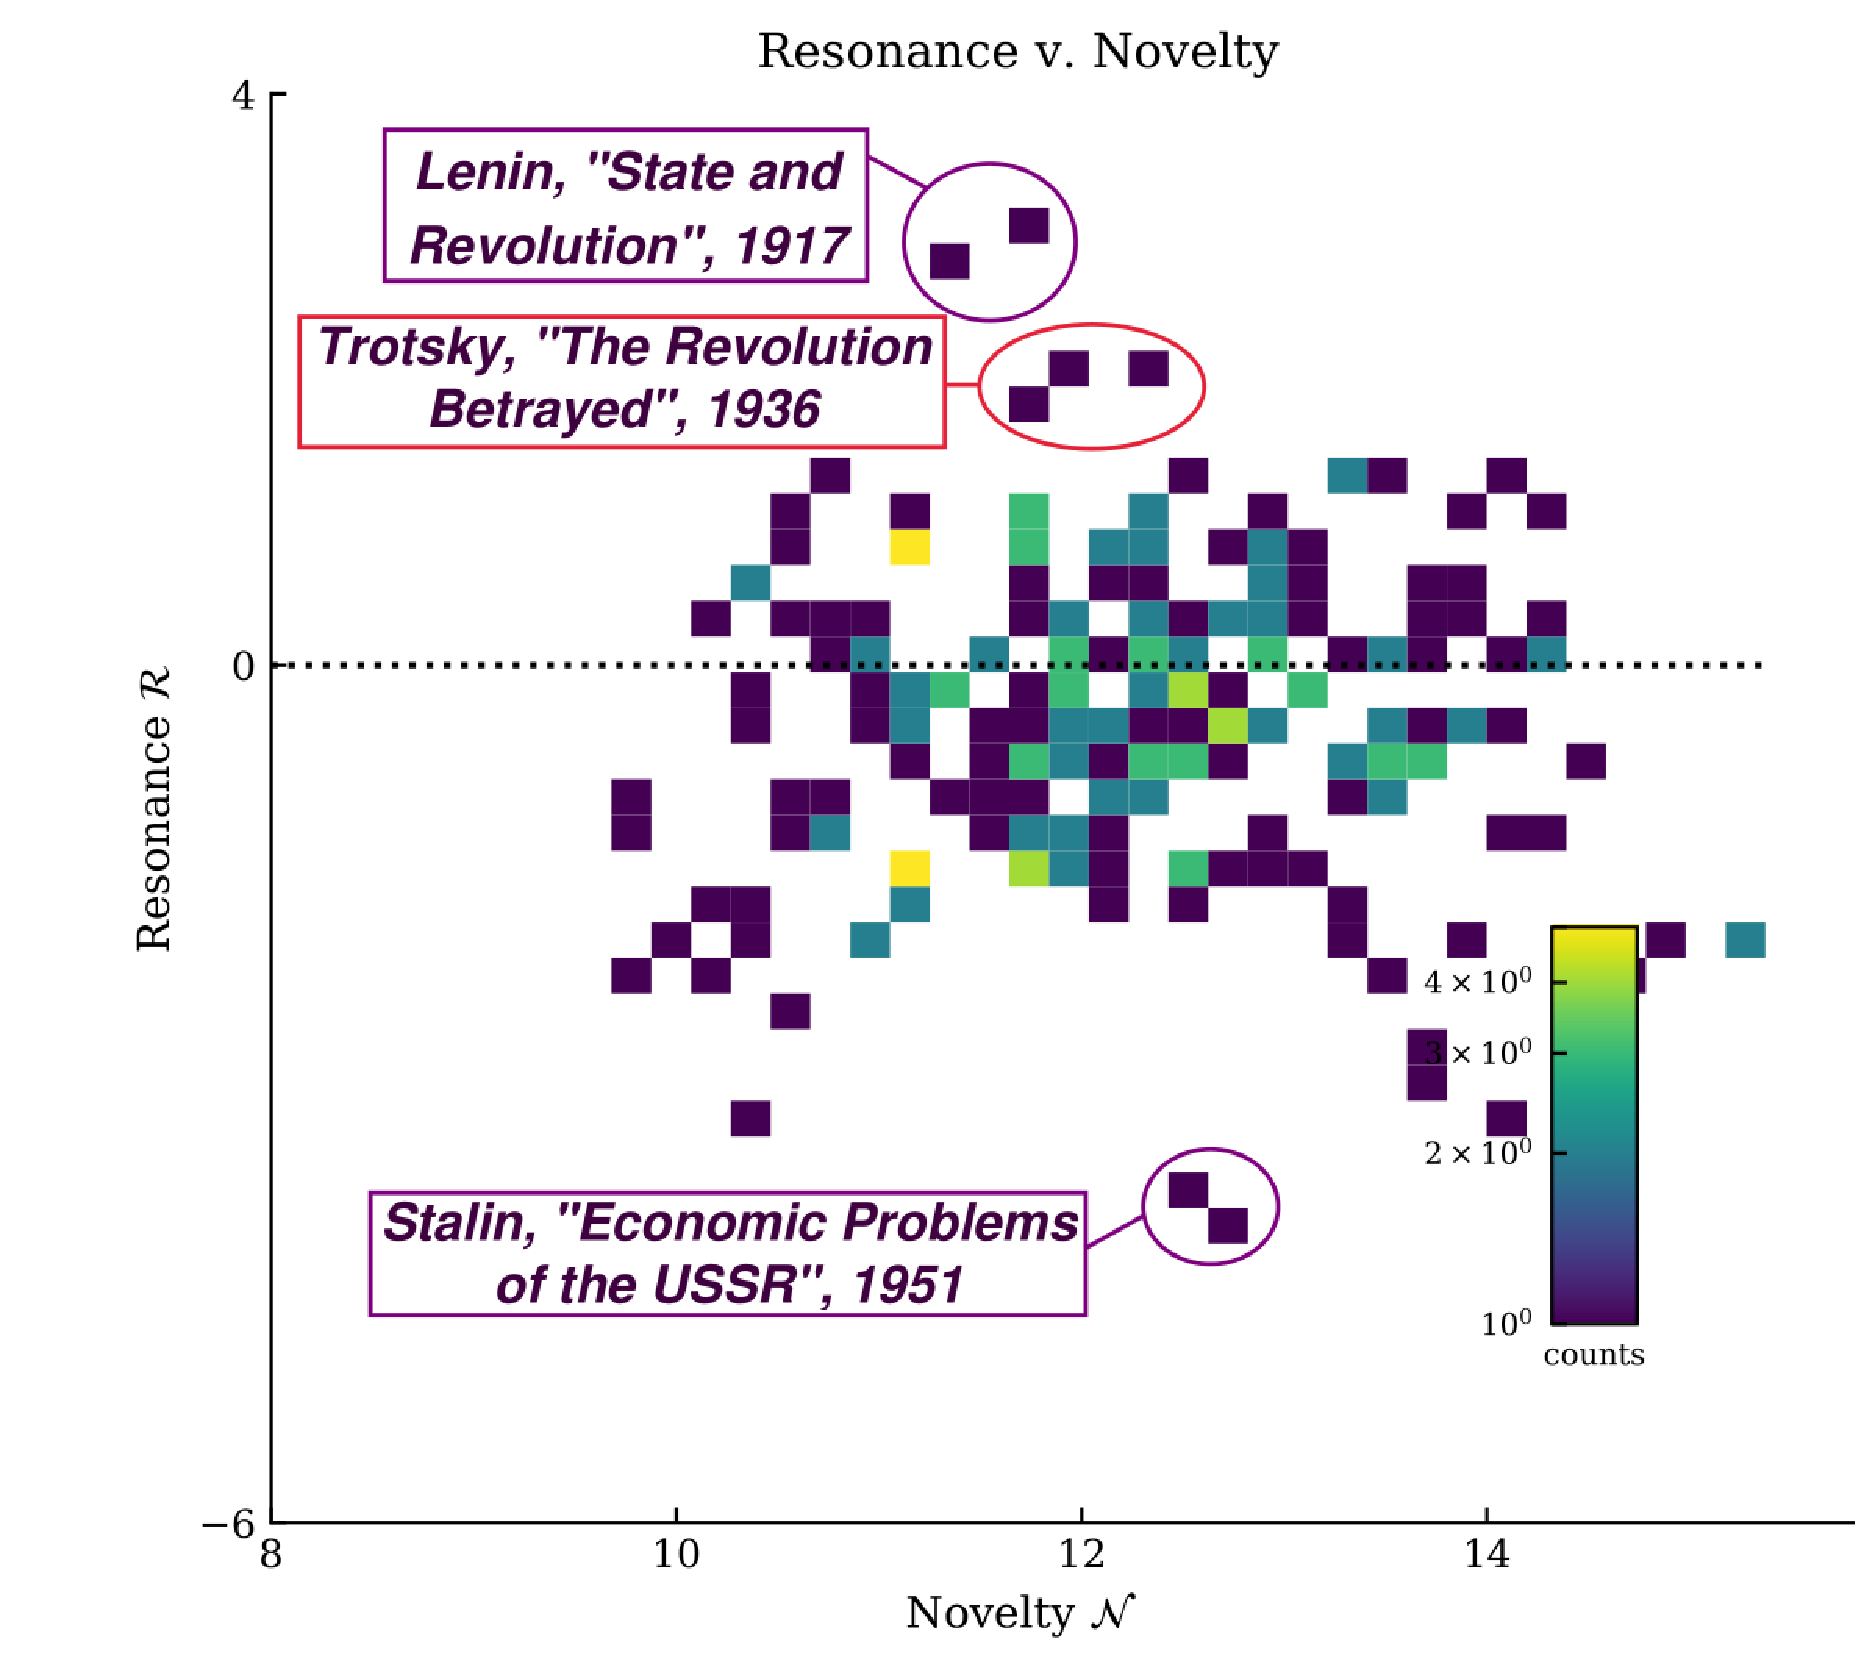
\includegraphics[width=\textwidth]{../figs/marxism_novelty_resonance.pdf}
	\caption{Novelty and resonance scores for each text in our corpus of influential Marxist texts.}
	\label{fig:novelty-resonance-marxism}
	\end{subfigure}
	\hfill
	\begin{subfigure}[t]{0.45\textwidth}
	\centering
	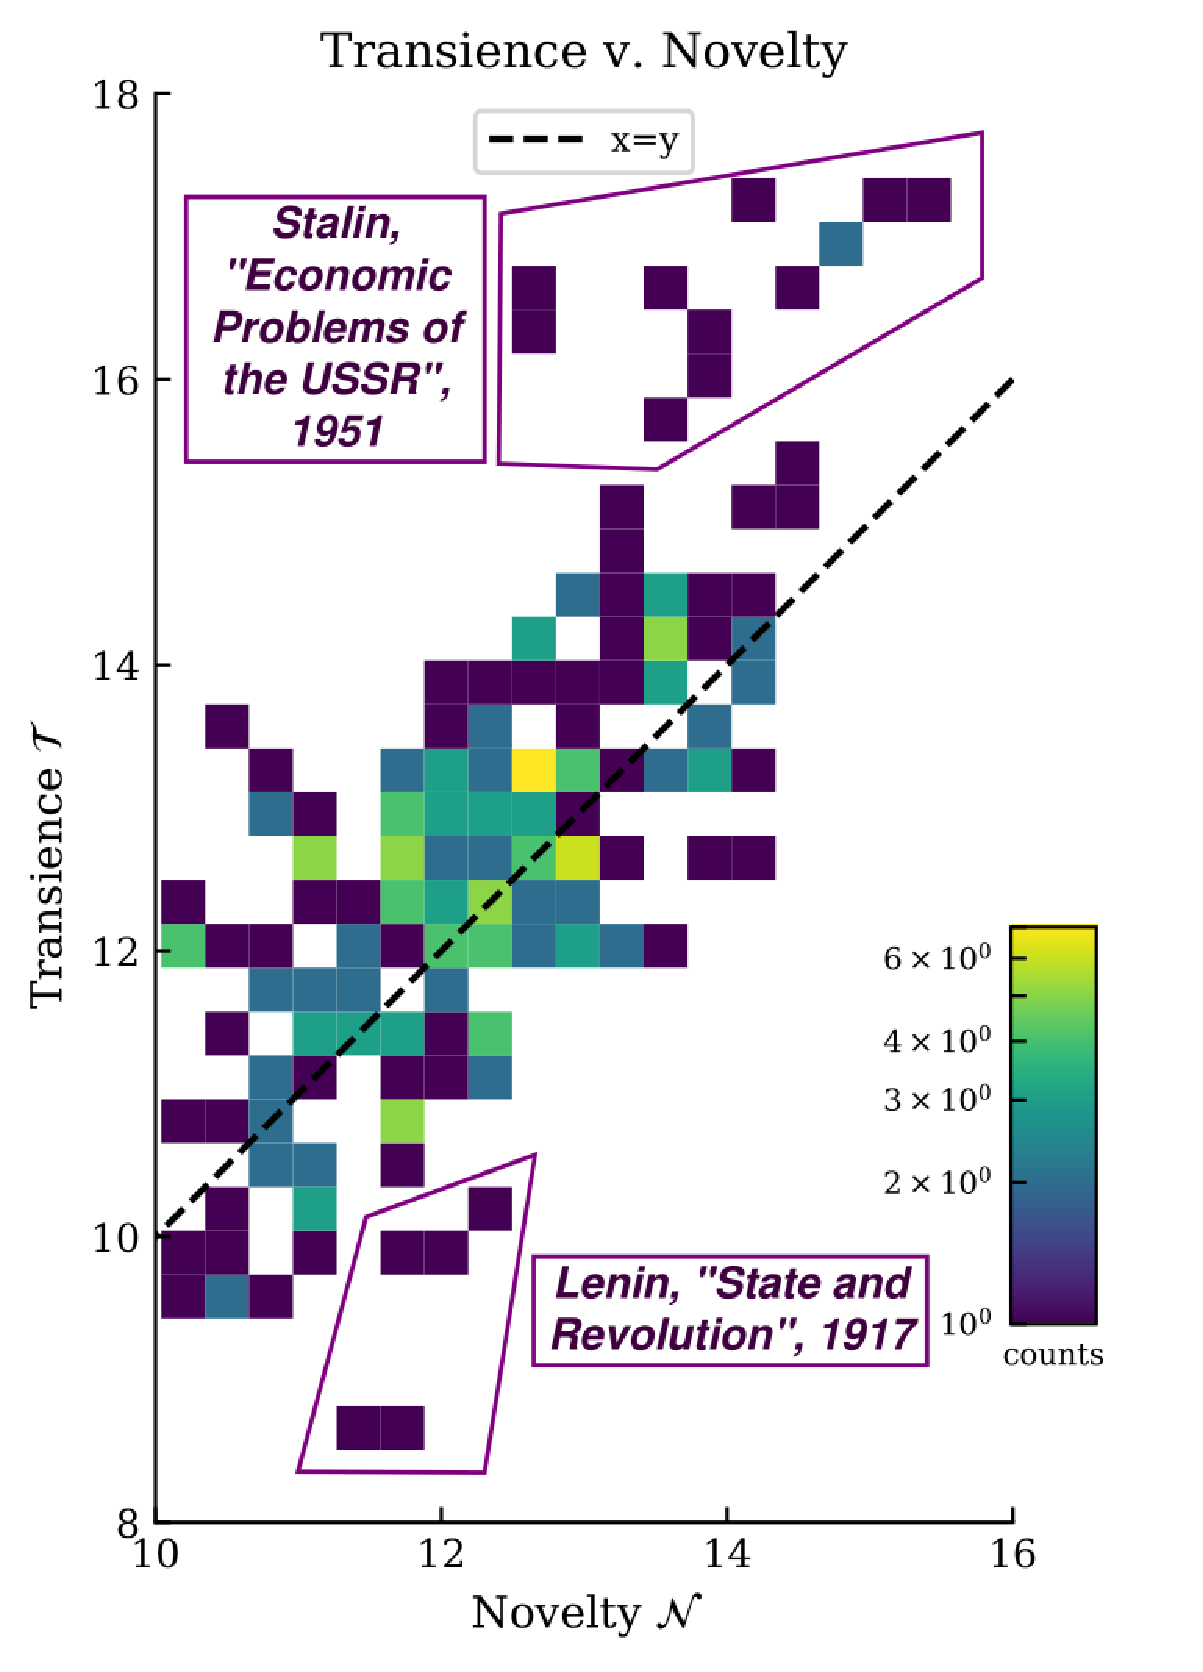
\includegraphics[width=0.8\textwidth]{../figs/marxism_transience_novelty.pdf}
	\caption{Transience and novelty scores for each text in our corpus of influential Marxist texts.}
	\label{fig:transience-novelty-marxism}
	\end{subfigure}
\end{figure}

%\subsubsection{Testing Models of Influence and Innovation with Synthetic Texts}

%Attempts to quantify influence and innovation, for example via scientometric ``impact'' scores for academic journals and scholars, are not new. In recent years, however, advances in Natural Language Processing have enabled researchers to study influence and innovation at the level of \textit{texts} themselves (\cite{barron_individuals_2018}, \cite{gerow_measuring_2018}), rather than textual metadata like citation and publication counts. While recent works in this vein have developed \textit{prima facie} plausible/reasonable models, little empirical work has been done to evaluate these models on the basis of commonsense understandings of influence and innovation, with studies instead relying upon likelihood functions derived endogenously from the models themselves. In this paper, then, we first develop a method for generating synthetic time-varying corpora with researcher control over the magnitude of influence $p$. We then use these corpora to test the influence models' ability to ``recover'' $p$, finding that []. We conclude with suggestions regarding what factors should be included in future models of influence and innovation, based upon a reading of the intellectual history literature in light of our findings.

\section{Conclusion}\label{sec:conclusion}

We began by introducing the hermeneutic background and inferential principles of the Cambridge School of historical analysis, and brought them into conversation with the computer science literature on contextual word embeddings. We showed how the latter not only \textit{implicitly} implements the Cambridge School methodology in a quantitative form but is in fact \textit{explicitly} linked to it through a shared history, which bifurcated into computational-linguistic and linguistic-philosophical strands in the 1950s, losing their shared language to an extent in the intervening years.

After describing these implicit and explicit connections, we dove more deeply into the details of how exactly computational embedding algorithms capture the contextual relationships between words: by constructing a geometric space mapping each word to a point such that points closer together share more contexts, or (in the case of the more recent \BERT{}-style models) mapping each word to a \textit{set} of points capturing different senses in which the word is used while still retaining the semantic meaning of distances between points.

We then took a quick detour through structuralist linguistics to explain the fundamental distinction between \textit{synchronic} and \textit{diachronic} modes linguistic analysis, to point out how these algorithms remain within the synchronic mode (modeling language as a single, static geometric space), and thus need to be paired with a diachronic model to constitute a sufficient tool for \textit{social-scientific} analysis of language. Considering \textit{influence} as the fundamental diachronic relationship of interest to historians of political thought, we reviewed theories and models of intellectual influence with the goal of identifying weaknesses in the standard Cambridge School approach (that is, the approach described in \cite{skinner_meaning_1969}), and constructed a new model able to overcome these weaknesses.

Next, to preview how this model can be employed towards fruitful analysis of historical texts, we walked through a series of introductory case studies, each one highlighting a particular feature of the model which our studies in the remaining chapters will take advantage of. In the mining-influence-claims case study, for example, we demonstrated a data-driven method for constructing an ontology of influence claims in the format of our model, focusing throughout on how assumptions regarding this ontology (for example, that \textsf{Collaboration} is a stronger influential force than \textsf{Shared-Geography}) can be transparently encoded---and then straightforwardly changed---as parameters within the model.
% developed a basic ontology of the types of influence that can be represented in the model

Finally, in the previous section, we introduced the Semantic Leadership Network model, which explicitly combines the synchronic embedding algorithms described in Section \ref{sec:methods-embeddings} and the diachronic influence model described in Section \ref{sec:methods-influence} by constructing \textit{networks} of embeddings where each node represents the embedding of author $a$'s writing at time $t$ and each edge is a connection between a time-$t$ node and a time-$t+1$ node, representing a potential instance of temporal influence. We concluded this section with the final three pieces of the puzzle, namely, (a) the mathematical formulation $\textsf{Lead}_{a_1 \rightarrow a_2}(w)$, which measures author $a_1$'s influence on author $a_2$ by way of their respective embeddings for a word $w$; (b) the method of edge-weighting by which the network of \textit{word}-level $\textsf{Lead}_{a_1 \rightarrow a_2}(w)$ scores is coarse-grained up to the level of author $\times$ time pairs (in our nomenclature, a network of $\textsf{Lead}^*_{a_1 \rightarrow a_2}$ scores); and (c) the use of the PageRank algorithm and its variants to derive our final author-influence scores.

By laying this groundwork---in particular, by walking through how the models emerge naturally
%in a piecewise fashion
from philosophical and social-scientific considerations, not from arrogant pretensions of automating or ``solving'' the process of historical inquiry---we hope to have preemptively quelled anxieties which may arise in the remaining chapters regarding what assumptions we're hiding in the machinery of the models, or what types of conclusions we are and are not comfortable drawing from their outputs. If we are successful in this endeavor, we hope in turn to have nudged the discussion around works of computational social science slightly away from these methodological fears and towards methodological possibilities for understanding political thought.
%and limitations.
% inherent to the practice of intellectual history, rather than 

\appendix

\section{Probabilistic Graphical Models in Political Theory}\label{sec:pgms}

\subsection{General Graphical Models}\label{sec:gms}

When trying to understand a complex historical phenomenon
%\footnote{Although we will sometimes use the term ``phenomenon'' throughout this work as a generic term for any object of investigation, we emphasize here that  Hempelian },
%complex phenomenon
one which involves lots of ``moving parts''---people, institutions, social relationships, and other related events---interacting to produce the event of interest, researchers are faced with the daunting task of where to begin their investigation. In this study we are indeed confronted with such a challenge, as we aim to understand the dynamics of three decidedly complex historical phenomena:
\begin{enumerate}
	\item the French Revolution,
	\item the intellectual origins of Marxism, and
	\item the spread of Marxism across Europe and, later, the Third World.
\end{enumerate}
Just as a mountain climber employs ``rules of thumb'' in deciding where to start their climb, in our study the following rule of thumb determines the course our investigation: that, to understand a complex historical phenomenon, the most fruitful way to make progress is to (a) break it down into its constituent elements, and then (b) specify how these elements work together to produce the phenomenon. This ``decompositional'' framework, we argue, corresponds naturally to a particular statistical framework known as Probabilistic Graphical Modeling. As we will argue below, this approach provides a method for transforming our \textit{intuitions} regarding events and their interrelationships into rigorous, measurable, and testable statistical \textit{hypotheses}.

A Probabilistic Graphical Model (PGM) is a statistical tool which, when paired with the laws of statistical inference, formalizes the decompositional framework we outlined above. Concretely, a PGM is a collection of nodes (drawn as circles), representing variables, and edges (drawn as arrows), representing relationships of influence between nodes---relationships which are then codified numerically in the form of ``Conditional Probability Tables''. This framework provides a level of abstraction that makes it invaluable for historical research, in that a wide range of historical-analytical frameworks can be subsumed (and thus formalized and tested) within it. Putting the ``probabilistic'' aspect aside for a moment, we can consider using a graphical model to begin a historical inquiry into the origins and eventual trajectory of the French Revolution, for example:
\begin{itemize}
	\item ``Mainstream'' historians can begin modeling the event by considering nodes for the Nobility, the Clergy, and the Third Estate, and edges for their pairwise interactions, as in Figure \ref{fig:fr-pgm-mainstream}.
	\item Marxist historians can instead consider the nodes to be the Bourgeoisie, the Proletariat, and the Peasantry, with edges again representing pairwise interactions, as in Figure \ref{fig:fr-pgm-marxist}.
	\item ``Great Men'' theorists can model prominent individuals as nodes: one for Louis XVI, another for Robespierre, a third for Napoleon, and so on, as in Figure \ref{fig:fr-pgm-greatman}. In this case, we see that \textit{not} all pairs of nodes have edges between them, since Louis XVI and Napoleon did not (at least, in a standard interpersonal sense) interact as part of the Revolution.
\end{itemize}

\begin{figure}[ht!]
	\centering
	\tikz{ %
		%\node[draw, rounded corners] (News) {Socialist Newspapers} ;
		\node[draw, rounded corners] (TE) {Third Estate} ; %
		\node[draw, rounded corners, above left=of TE] (N) {Nobility} ;
		\node[draw, rounded corners, above right=of TE] (C) {Clergy} ;
		\node[right=of C] (MSP) {\textit{More Social Power}} ;
		\node[below=of MSP] (LSP) {\textit{Less Social Power}} ;
		%\node[latent, right=of w] (a) {$a$} ; %
		\edge[<->] {TE} {N} ;
		\edge[<->] {TE} {C} ;
		\edge[<->] {N} {C} ;
		\edge {LSP} {MSP} ;
	}
	\caption{A graphical model illustrating the initial decomposition which a historian of the French Revolution might perform to make their analysis more tractable: three nodes representing three historical entities---the Nobility, the Clergy, and the Third Estate---and edges representing the interrelationships between each pair of entities.}
	\label{fig:fr-pgm-mainstream}
\end{figure}

\begin{figure}[ht!]
	\centering
	\tikz{ %
		%\node[draw, rounded corners] (News) {Socialist Newspapers} ;
		\node[draw, rounded corners] (B) {Bourgeoisie} ; %
		\node[draw, rounded corners, below=of B] (Pr) {Proletariat} ;
		\node[draw, rounded corners, right=of B] (LG) {Landed Gentry} ;
		\node[draw, rounded corners, below=of LG] (Pe) {Peasantry} ;
		\node[below=of Pr,yshift=5mm] (Urb) {\textit{Urban}} ;
		\node[right=of Urb,xshift=13mm] (Rur) {\textit{Rural}} ;
		\node[right=of LG,xshift=-5mm] (MSP) {\textit{More Social Power}} ;
		\node[below=of MSP] (LSP) {\textit{Less Social Power}} ;
		%\node[latent, right=of w] (a) {$a$} ; %
		\edge[<->] {B} {Pr} ;
		%\edge[<->] {B} {Pe} ;
		\edge[<->] {B} {LG} ;
		\edge[<->] {Pr} {Pe} ;
		\edge[<->] {LG} {Pe} ;
		\edge[<->] {Urb} {Rur} ;
		\edge {LSP} {MSP} ;
	}
	\caption{A graphical model illustrating the initial decomposition which a Marxist historian of the French Revolution might perform to make their analysis more tractable: three nodes representing three historical entities---the Bourgeoisie, the Proletariat, and the Peasantry---and edges representing the interrelationships between each pair of entities.}
	\label{fig:fr-pgm-marxist}
\end{figure}

\begin{figure}[ht!]
	\centering
	\tikz{ %
		%\node[draw, rounded corners] (News) {Socialist Newspapers} ;
		\node[draw, rounded corners] (AB) {A. Barnave} ;
		\node[draw, rounded corners, above=of AB] (M) {Mirabeau} ;
		\node[draw, rounded corners, left=of AB,xshift=1mm] (MA) {Marie Antoinette} ;
		\node[draw, rounded corners, above=of MA] (L) {Louis XVI} ;
		\node[draw, rounded corners, above right=of AB] (R) {Robespierre} ;
		\node[draw, rounded corners, below=of R] (MR) {Mme Roland} ;
		\node[draw, rounded corners, above right=of MR] (PB) {P. Barras} ;
		\node[draw, rounded corners, below=of PB] (GB) {G. Babeuf} ;
		\node[draw, rounded corners, right=of PB] (N) {Napoleon} ;
		\node[below=of MR,yshift=8mm] (Time) {\textit{Time}} ;
		\node[right=of Time] (BlankR) {$~$} ;
		\node[left=of Time] (BlankL) {$~$} ;
		\node[below=of L,yshift=6.5mm,xshift=-18mm] (DotL) {} ;
		\node[below=of N,yshift=6.5mm,xshift=12mm] (DotR) {} ;
		%\node[above=of AB,yshift=-5mm] (Rul) {\textit{(Held Power)}} ;
		%\node[latent, right=of w] (a) {$a$} ; %
		\edge[<->] {L} {MA} ;
		\edge[<->] {L} {AB} ;
		\edge[<->] {L} {M} ;
		\edge[<->] {M} {AB} ;
		\edge[<->] {M} {MA} ;
		\edge[<->] {M} {R} ;
		\edge[<->] {MA} {AB} ;
		\edge[<->] {AB} {MR} ;
		\edge[<->] {R} {AB} ;
		\edge[<->] {R} {MR} ;
		\edge[<->] {R} {PB} ;
		\edge[<->] {PB} {GB} ;
		\edge[<->] {PB} {N} ;
		\edge[<->] {N} {GB} ;
		\edge {Time} {BlankR} ;
		\edge[-] {BlankL} {Time} ;
		\edge[-, dashed] {DotL} {DotR} ;
	}
	\caption{A graphical model illustrating the initial decomposition which a ``Great Man'' theorist might perform to make their analysis of the French Revolution more tractable, with nodes for prominent individuals and edges between individuals who are known to have interacted.}
	\label{fig:fr-pgm-greatman}
\end{figure}

As these figures demonstrate, graphical models provide the researcher with a vast set of modeling possibilities: nodes can represent people, classes, institutions, or other units of observation, while edges can represent interpersonal interactions, economic relations, or any other dyadic relationships between nodes\footnote{In fact, although the probabilistic aspect of PGMs---the ability to derive statistical inferences regarding the nodes and their interactions---requires edges to be dyadic, for the purposes of non-probabilistic modeling one can introduce ``hyperedges'' representing a relationship between any number of nodes. The Clandestine Cell Structure of modern insurgent groups, for example, can be modeled effectively using hyperedges, since it is the holistic relationship among \textit{all} members of a cell, rather than the individual dyadic relationships between them, that is most relevant to the functioning of the structure:
	\begin{center}
		\tikz{ %
			% Top
			\node[draw, rounded corners] (NL) {Network Leader} ;
			% Second Level
			\node[draw, rounded corners, below left=of NL,yshift=5mm] (BL1) {Branch Leader} ;
			\node[draw, rounded corners, below right=of NL,yshift=5mm] (BL2) {Branch Leader} ;
			% Cells
			\factor[below left=of BL1,xshift=-4mm,yshift=-8mm]{CA}{}{}{};
			\node[draw, rounded corners, left=of CA] (CAM1) {Alice} ;
			\node[draw, rounded corners, below left=of CA] (CAM2) {Arturo} ;
			\node[draw, rounded corners, below=of CA] (CAM3) {Andrew} ;
			\node[draw,dashed,fit=(CA)(CAM1)(CAM2)(CAM3)] {};
			\factor[below right=of BL1,xshift=-5mm,yshift=-8mm]{CB}{}{}{} ;
			\node[draw, rounded corners, left=of CB] (CBM1) {Bob} ;
			\node[draw, rounded corners, below left=of CB] (CBM2) {Bill} ;
			\node[draw, rounded corners, below=of CB] (CBM3) {Barry} ;
			\node[draw, rounded corners, below right=of CB] (CBM4) {Betty} ;
			\node[draw, rounded corners, right=of CB] (CBM5) {Bruce} ;
			\node[draw,dashed,fit=(CB)(CBM1)(CBM2)(CBM3)(CBM4)(CBM5)] {};
			\factor[below left=of BL2,xshift=-3.5mm,yshift=-7mm]{CC}{}{}{} ;
			\node[draw, rounded corners, below left=of CC,xshift=8mm] (CCM1) {Chris} ;
			\node[draw, rounded corners, below right=of CC,xshift=-8mm] (CCM2) {Cathy} ;
			\node[draw, dashed, fit=(CC)(CCM1)(CCM2)] {} ;
			\factor[below right=of BL2,xshift=4mm,yshift=-8mm]{CD}{}{}{} ;
			\node[draw, rounded corners, left=of CD,xshift=2mm] (CDM1) {Derek} ;
			\node[draw, rounded corners, right=of CD,xshift=-2mm] (CDM2) {Don} ;
			\node[draw, rounded corners, below left=of CD,xshift=2mm] (CDM3) {Dana} ;
			\node[draw, rounded corners, below right=of CD,xshift=-2mm] (CDM4) {Drew} ;
			\node[draw, dashed, fit=(CD)(CDM1)(CDM2)(CDM3)(CDM4)] {} ;
			%	    \node[draw, rounded corners, below=of trinity] (HS) {\shortstack{Holy\\Spirit}} ;
			%	    \node[draw, rounded corners, above left=of trinity] (F) {Father} ;
			%	    \node[draw, rounded corners, above right=of trinity] (S) {Son} ;
			%	    \node[draw,dashed,fit=(HS) (F) (S)] {};
			%		%\node[above=of AB,yshift=-5mm] (Rul) {\textit{(Held Power)}} ;
			%		%\node[latent, right=of w] (a) {$a$} ; %
			\edge[->] {NL} {BL1} ;
			\edge[->] {NL} {BL2} ;
			\edge[->] {BL1} {CA} ;
			\edge[->] {BL1} {CB} ;
			\edge[-] {CA} {CAM1} ;
			\edge[-] {CA} {CAM2} ;
			\edge[-] {CA} {CAM3} ;
			\edge[-] {CB} {CBM1} ;
			\edge[-] {CB} {CBM2} ;
			\edge[-] {CB} {CBM3} ;
			\edge[-] {CB} {CBM4} ;
			\edge[-] {CB} {CBM5} ;
			\edge[->] {BL2} {CC} ;
			\edge[->] {BL2} {CD} ;
			\edge[-] {CC} {CCM1} ;
			\edge[-] {CC} {CCM2} ;
			\edge[-] {CD} {CDM1} ;
			\edge[-] {CD} {CDM2} ;
			\edge[-] {CD} {CDM3} ;
			\edge[-] {CD} {CDM4} ;
			%		\edge[-] {trinity} {S} ;
		}
	\end{center}
	
	%The Christian doctrine of the Trinity, for example, could be modeled as a triadic relationship between Father, Son, and Holy Spirit (unlike in the case of dyadic edges, which can be represented via arrows, hyperedges are typically represented via a dotted region containing all the $n$ nodes which comprise the $n$-ary relationship):
	%\begin{center}
	%\tikz{ %
		%	    %\node[draw, rounded corners] (HS) {\begin{tabular}{c} Holy \\ Spirit\end{tabular}} ;
		%	    \factor[]{trinity}{}{}{};
		%	    \node[draw, rounded corners, below=of trinity] (HS) {\shortstack{Holy\\Spirit}} ;
		%	    \node[draw, rounded corners, above left=of trinity] (F) {Father} ;
		%	    \node[draw, rounded corners, above right=of trinity] (S) {Son} ;
		%	    \node[draw,dashed,fit=(HS) (F) (S)] {};
		%		%\node[above=of AB,yshift=-5mm] (Rul) {\textit{(Held Power)}} ;
		%		%\node[latent, right=of w] (a) {$a$} ; %
		%		\edge[-] {trinity} {HS} ;
		%		\edge[-] {trinity} {F} ;
		%		\edge[-] {trinity} {S} ;
		%	}
	%\end{center}
}. In addition, given the graphical representation, the \textit{position} of the nodes in 2D space can also be used to represent divisions or axes of differentiation: in the case of Figure \ref{fig:fr-pgm-marxist}, for example, moving left to right represents moving from urban-situated to rural-situated entities, while moving from bottom to top represents moving in the direction of increased social power. Similarly, in Figure \ref{fig:fr-pgm-greatman}, moving left to right represents the passage of time (with nodes positioned based on when, in the course of the revolution, their role was most prominent), and the nodes are divided vertically into two groups based on whether or not the individual was the main political ruler of France at a given time. With only a few nodes this spatial organization may seem like more trouble than it's worth, but it becomes immensely helpful as the model becomes more and more complex. For example, if the Marxist researcher aimed to subsequently model the Soviet subdivision of the Peasantry into \textit{bednyak}, \textit{serednyak}, \textit{kulak}, and \textit{batrak} classes, the \textit{batrak} class could be placed somewhere in the middle of the rural-urban axis, as members of this class often migrated seasonally between urban and rural work.

As these examples show, Graphical Modeling provides a powerful tool for developing explanatory theories of historical phenomena, in forcing the researcher to think simultaneously about (a) what the relevant entities are and (b) what types of relationships exist among them. Thus far, however, we have left out the ``probabilistic'' aspect of the models used throughout this paper, by remaining agnostic about what particular types of relationships are admissible in these models. Now that we've shown the usefulness of general Graphical Modeling for theory development, in the next section we show---by way of an introduction to text-analytic topic models---how \textit{Probabilistic} Graphical Modeling further enhances the researcher's toolkit, by enabling principled statistical inferences to be drawn regarding the interrelationships between nodes in a Graphical Model.

\subsection{The Role of Probability}\label{sec:probability}

While in the previous section we restricted our examples to general historical modeling, in this section we turn to the use of \textit{textual} data in conducting a historical study, and in the process show how the probabilistic aspect of the Probabilistic Graphical Model allows us to reason in a statistically-principled manner about what a given corpus of texts tells us about the historical phenomena we're interested in studying.

The first step in a researcher's journey towards understanding a textual corpus is to develop a rough schema of topics covered in the corpus, to figure out what each text is ``about'', and to group the texts accordingly. This thematic categorization, the act of transforming an archive of texts into one partitioned into sections, often takes up a massive chunk of research time and resources. Given this resource bottleneck, this transformation is precisely what one of the first text analysis methods, Latent Semantic Analysis (LSA), was created to do, and (somewhat miraculously) it does so without any input required from the researcher besides having the texts in some digitized format.

Scale-wise, LSA is already leaps and bounds beyond human capabilities, but we can do better: in 2003, David Blei, Andrew Ng, and Michael I. Jordan developed an extension to LSA called Latent Dirichlet Analysis (LDA), which ``zooms in'' on each document and actually learns distributions over topics for each token (word). That is, while LSA places each document into a single category, LDA derives a more detailed summary of each document, like ``25\% of this document is about computer science and 75\% is about linguistics,'' a more realistic model given the tendency for most written documents to range across multiple topics (for example, a news article introducing a new technology and then discussing its potential societal impact). In fact, if a researcher does want a single category for each document, they can simply choose the topic with the highest proportion: linguistics, in the case of our example document.

%This represents, in our view, nothing short of a revolution for social science research.

For a researcher hoping to study taxation practices in \textit{ancien régime} France, for example, this means the difference between reading through \textit{every} text in the archive and reading only the specific subset of the texts which are known to discuss the topic of taxation. Depending on the time and resources available to the researcher, for example, they can read the $N$ documents with the highest proportions devoted to taxation: the more resources are available, the higher this $N$ can be.

Both LSA and LDA fall into the category of ``unsupervised'' algorithms, given the lack of user intervention in the topic-learning process. While this approach stays true to the idea of ``pure'' exploratory data analysis, it is rare for a researcher to have absolutely no idea what topics lie within an archive. More commonly, researchers come to the texts with a rough set of topics in mind and want to see which texts fall within these topics, thus shifting the nature of the research more towards confirmatory data analysis. In this case, they can use a ``semi-supervised'' Labeled LDA algorithm like CorEx \citep{gallagher_anchored_2017}, which allows them to ``suggest'' salient topics to the LDA algorithm before it runs. In our French \textit{ancien régime} example, Labeled LDA would allow researchers to suggest single keywords like ``impôts'' (taxes) or keyword groups like \{``gabelle'', ``taille''\} (the salt tax and the land tax, respectively, two of the most onerous \textit{ancien régime} tax burdens in the eyes of the peasantry), thus nudging the LDA algorithm towards detecting taxation-related topics.

%A third class of text-analysis algorithms, called supervised algorithms, re probably the most studied and widely-used. In direct confirmatory analysis, the existence of a pre-existing codebook or categorization scheme for a corpus of interest opens up even more possibilities. Though a wide variety of supervised text analysis algorithms exist, their common goal is to learn an existing user-specified categorization scheme given only a small subset of the full corpus which has been pre-categorized, aiming to learn a categorization function which best generalizes to the larger universe of texts in the corpus. If the corpus contains one million documents, for example, the researcher could randomly sample 1000 documents from the larger corpus and manually label them using their codebook, give 800 of these documents to the algorithm as training data, then evaluate the learned classification function using the remaining 200 documents (never shown to the learning algorithm) as test data\footnote{The 800/200 split is not an arbitrary choice: this 80/20 split is recommended by most practitioners in the absence of any information about how easily the categorization scheme can be learned from a certain number of documents. This is not a mathematically-justified ``rule'', however—just a heuristic or ``rule of thumb''. Researchers with simpler categorization schemes could instead set aside 10 percent or less of the documents as training data.}.

%But how exactly should we evaluate the classifier? While an intuitive measure of ``success'' is the accuracy rate of its predicted label for the 200 test documents, intuition fails in this case. A very undesirable classifier, from the researcher's perspective, could in fact still maximize this quantity. For example, if 90\% of all the documents in the corpus are about computer science, an algorithm which just guessed the label ``computer science'' for every document it ever saw would do extremely well with respect to this measure (it would be correct 90\% of the time), while failing to actually learn anything substantive about the categorization scheme. Thus, instead, computer scientists typically evaluate these learned functions using the F1 score, which incorporates both the classifier's false-positive and false-negative rates, avoiding this type of degenerate case.

But how exactly are these algorithms able to detect topics within a corpus without being given any domain-specific knowledge whatsoever? This seeming miracle is achieved, in short, via a statistical model of the writing process: since texts tend to be structured---into sentences, paragraphs, and chapters, for example---in such a way that a given section (say, a paragraph) focuses on only one or a few topics selected from the much wider set of topics existing across the corpus, we can infer that the more a pair of words co-occurs \textit{within} these sections the more likely they are to pertain to the same topic. At a high level, therefore, we can scan over a corpus and discover its constituent topics simply by identifying clusters of words that tend to occur close to one another. A topic then, in this sense, is ``coherent'' to the extent that its words are more likely to co-occur than we would expect by ``random chance''---i.e., if the words were randomly selected one-by-one from a dictionary. This captures the intuition that, for example, since the Wikipedia article for Thomas Hobbes is about a particular topic, words which occur \textit{within} this article (choosing eight at random, programmatically) are more likely to be about the same topic than words chosen at random across all words in all Wikipedia articles (again choosing eight at random, programmatically), as illustrated in Table \ref{tab:hobbes-wiki}.

% economic, rebellions, converted, mode, right-wing, countries, struggle, believed

\begin{table}[ht!]
	\centering
	\begin{tabular}{ccc}
		\toprule
		\textbf{Thomas Hobbes} & \textbf{Karl Marx} & \textbf{All Wikipedia} \\
		\midrule
		war & economic & wolf \\
		civil & rebellions & chondrite \\
		consent & converted & bawdy \\
		among & mode & larynx \\
		patriarchalists & right-wing & perchance \\
		history & countries & cytosine \\
		enter & struggle & pollinate \\
		government & industrialisation & negligible \\
		\bottomrule
	\end{tabular}
	\caption{Randomly-chosen words from Wikipedia articles on Thomas Hobbes and Karl Marx, versus randomly-chosen words from across all Wikipedia articles}
	\label{tab:hobbes-wiki}
\end{table}

Concretely, for reasons which will be elucidated in the next section, we can transform this intuition into a computationally-estimable model by specifying a ``data-generating process''---essentially a stylized story of how the author ``chose'' the sequences of words which appear in the texts. For example, previewing what is to come, Algorithm \ref{alg:text-corpus} represents the basic data-generating process underlying all topic models.

\begin{algorithm}[ht!]
	\caption{Data-Generating Process for a Text Corpus}
	\label{alg:text-corpus}
	\begin{enumerate}
		\item \textit{Choose hyperparameters}. The author decides how many documents $N$ they'd like to write, as well as a set of $K$ topics they'd like to write about in these texts. We assume the author has a vocabulary of $M$ words $V = \{w_1, w_2, \ldots, w_M\}$ to draw on while writing.
		\item \textit{Specify topics}. For each topic $t \in \{t_1, t_2, \ldots, t_K\}$, the author evaluates which words in $V$ are most and least pertinent. For example, if the topic is astronomy, ``planet'', ``moon'', and ``orbit'' will be given high scores, while ``koala'' and ``headache'' will be given low scores. Each topic $t$ is thus assigned a corresponding set of importance scores for each word: $p_t(v)$ represents the importance to topic $t$ of word $v$. In our example, the author may choose $p_t(\texttt{planet}) = p_t(\texttt{moon}) = p_t(\texttt{orbit}) = 0.3$, and $p_t(\texttt{koala}) = p_t(\texttt{headache}) = 0.05$.
		\item \textit{Specify documents}. For each document $d \in \{d_1, d_2, \ldots, d_N\}$, the author chooses
		\begin{enumerate}
			\item how many words $N_d$ they'd like to write for this document, thus creating blank slots $S_d = \{s_{d,1}, s_{d,2}, \ldots, s_{d,N_d}\}$, and
			\item the distribution of topics $\theta_d$ they'd like to cover in this document. For example, if $d$ is an article on the Franco-Prussian War, they might choose $\theta_d$ to be a balance between three topics: 40\% France, 40\% Prussia, and 20\% warfare. Mathematically, if the global set of topics $T$ chosen in Step 1 was $t_1 = \text{France}$, $t_2 = \text{Prussia}$, $t_3 = \text{warfare}$, $t_4 = \text{Buddhism}$, this balance would be represented by $\theta_d = (0.4, 0.4, 0.2, 0.0)$.
		\end{enumerate}
		\item \textit{Fill the documents with words}. For each slot $s_{d,i}$ in a document $d$, the author chooses a topic for this slot $t_{d,i}$ based on the document's topic distribution $\theta_d$ (the distribution chosen in the previous step). They then choose a word $w$ from their vocabulary $V$ to fill in this slot, with the probability of choosing a specific word $w_j$ proportional to that word's topic-$t_{d,i}$ importance score $p_{t_{d,i}}(w_j)$.
	\end{enumerate}
\end{algorithm}

Despite the simplicity of this model, its definition of a topic as a grouping of words precisely captures the word co-occurrence intuition from above: rather than choosing words at random, as in the All Wikipedia column of Table \ref{tab:hobbes-wiki}, the author first chooses a \textit{topic}, which thus establishes the likelihood that particular words are chosen. In this way, continuing our example, choosing the Thomas Hobbes topic increases the likelihood that the term ``civil'' is chosen to be the next word in the text (relative to its frequency in the English language in general), whereas choosing the Karl Marx topic would instead make ``industralisation'' more likely to be chosen (again, relative to its overall frequency in English).

Once this data-generating process is specified, all that is left to do for a computer to discover the latent topics within a corpus is to ``run it backwards'': in essence, to divide the words in the texts up into clusters which best fit this story. Putting ``chondrite'' and ``cytosine'' (the first being a type of meteorite, the second a nucleotide found in DNA) into the same cluster, for example, would not fit the story well, since these terms will rarely co-occur in the same section of a text. If it instead placed ``chondrite'' into a cluster with other astronomy terms and ``cytosine'' into a separate cluster of microbiological terms, this would better explain the tendency for words in the former to co-occur in texts about astronomy, and for words in the latter to co-occur in texts about microbiology.

The fact that a computer is able to estimate this ``best'' division in mere seconds (i.e., without trying every single possible split of the vocabulary into separate word clusters, which would be prohibitively time-consuming and computationally expensive) is due to the magic of Probabilistic Graphical Models (PGMs), algorithms which allow researchers to specify the parameters of their data-generating processes---\textit{any} data-generating processes which adhere to a loose set of constraints---and nearly instantly obtain estimates for the parameters within these specifications. In the case of general topic models, for example, the basic parameters would be (a) the distribution of \textit{topics} across the corpus, and (b) the distribution of \textit{words} within each topic. By restricting the total number of topics $K$ that we want the algorithm to generate, we force it to choose a small set of coherent topics, based on the $K$ word clusters with the strongest co-occurrence patterns. In the next section we introduce the specific form that these Probabilistic Graphical Models take, and walk through an example of how they can be constructed around a set of hypotheses.

%, since although the studies of the \textit{cahiers de dolèances} in Chapter \ref{ch:cahiers} employ a wide range of different topic models, all of them can in fact be understood as small variations on a ``base'' topic model PGM.

\begin{figure}
	\centering
	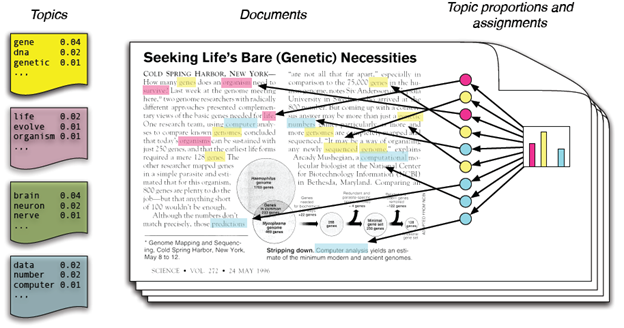
\includegraphics[width=\textwidth]{../figs/blei_lda.png}
	\caption{From \cite{blei_introduction_2012}, p. 3}
	\label{fig:my_label}
\end{figure}

Every such PGM is simply the formal mathematical representation of a data-generating process, such as the text-generation process described above in Algorithm \ref{alg:text-corpus}. So, if we wanted to model the relationship between weather and a person's choice of whether to go out and party or stay in and watch a movie on a given Saturday evening, we could begin by proposing the data-generating process given in Algorithm \ref{alg:party-weather}.

\begin{algorithm}[ht!]
	\caption{Data-Generating Process for Evening Plans}
	\label{alg:party-weather}
	\begin{enumerate}
		\item The person $P$ looks out the window and observes the weather.
		\item If the weather is sunny, $P$ goes out to a party. Otherwise, $P$ stays in and watches a movie.
	\end{enumerate}
\end{algorithm}

Now, given the description of a PGM given above (nodes as variables, edges as relationships between variables), we can perform the move alluded to in the previous section: we can convert our data-generating process into a PGM, by defining nodes (variables) and edges (relationships) as follows:

\begin{enumerate}
	\item A variable $w$ which can take on values in $\{\textsf{Sunny}, \textsf{Rainy}\}$
	\item A variable $a$ which can take on values in $\{\textsf{Go Out}, \textsf{Stay In}\}$, and 
	\item An edge $e$ from $w$ to $a$ which encodes the intuition that one is more likely to go out if it's sunny than if it's rainy via the probability distribution $P(\textsf{Go Out} \; | \; \textsf{Sunny}) = 0.75$, $P(\textsf{Stay In} \; | \; \textsf{Sunny}) = 0.25$, $P(\textsf{Go Out} \; | \; \textsf{Rainy}) = 0.25$, and $P(\textsf{Stay In} \; | \; \textsf{Rainy}) = 0.75$.
\end{enumerate}

The resulting PGM, in graphical form\footnote{The ``Graphical'' in Probabilistic Graphical Model is not used in the same sense as the ``graphical'' we're used to from vernacular English. Capital-G Graphical denotes that the Probabilistic Model is represented as a Graph, a well-defined mathematical object consisting of nodes and edges, which does not have to be represented graphically (though it could be, like in our example here with circles and arrows). In fact, when a computer program is estimating a PGM, it is by definition not in a graphical form---it's in the form of 0s and 1s, stored in the computer's memory.}, is presented in Figure \ref{fig:pgm1}, where the Conditional Probability Table describing the edge from the $w$ node to the $a$ node is given in Table \ref{tab:cpt1}.

\begin{figure}[ht!]
	\centering
	\tikz{ %
		\node[latent] (w) {$w$} ; %
		\node[latent, right=of w] (a) {$a$} ; %
		\edge {w} {a} ;
	}
	\caption{A basic PGM, representing the relationship between $w$, the weather, and $a$, the subsequent action of a person deciding whether to go out or stay in for the night.}
	\label{fig:pgm1}
\end{figure}

%\begin{figure}
%    \centering
%    \includegraphics{fig3.png}
%    \caption{A basic PGM, representing the relationship between $w$, the weather, and $a$, the subsequent action of a person deciding whether to go out or stay in for the night.}
%    \label{fig:pgm1}
%\end{figure}

\begin{table}[ht!]
	\centering
	\begin{tabular}{c|cc}
		& \textsf{Go Out} & \textsf{Stay In} \\\hline
		\textsf{Sunny} & 0.75 & 0.25 \\
		\textsf{Rainy} & 0.25 & 0.75 \\
	\end{tabular}
	\caption{The Conditional Probability Table for the PGM shown in Figure \ref{fig:pgm1}.}
	\label{tab:cpt1}
\end{table}

PGMs can help us make inferences about the world in the face of incomplete information, which is the situation in nearly every real-world problem. The key tool here is the separation of nodes into two categories: \textit{observed} (represented graphically as a shaded node) and \textit{latent} (represented graphically as an unshaded node). Thus we can now use our model as a weather-inference machine: if we observe that the person we're modeling is out at a party with us, what can we infer from this information about the weather outside? We can draw this situation as a PGM with shaded and unshaded nodes, as in Figure \ref{fig:pgm2}, and then use Bayes' Rule to perform calculations over the network, to see how the observed information about the person at the party ``flows'' back into the node representing the weather.

\begin{figure}[ht!]
	\centering
	\tikz{ %
		\node[latent] (w) {$w$} ; %
		\node[obs, right=of w] (a) {$a$} ; %
		\edge {w} {a} ;
	}
	\caption{A PGM representing the same situation as in Figure \ref{fig:pgm1}, except that the node for variable $a$ is now shaded, indicating a situation where we have observed the person's action ($a = \textsf{Go Out}$) but still only have a probability distribution over the weather $w$.}
	\label{fig:pgm2}
\end{figure}

%\begin{figure}
%    \centering
%    \includegraphics{fig4.png}
%    \caption{A PGM representing the same situation as in Figure \ref{fig:pgm1}, except that the node for variable $a$ is now shaded, indicating a situation where we have observed the person's action ($a = \textsf{Go Out}$) but still only have a probability distribution over the weather $w$.}
%    \label{fig:my_label}
%\end{figure}

Keeping in mind that Bayes' Rule tells us, for any two events $A$ and $B$, how to use information about $P(B|A)$ to obtain information about $P(A|B)$:
\begin{align*}
	P(A | B) = \frac{P(B | A)P(A)}{P(B)},
\end{align*}
We can now apply this rule to obtain our new probability distribution over the weather, taking into account the new information that the person has chosen to go out:
\begin{align*}
	P(w = \textsf{Sunny} \; | \; a = \textsf{Go Out}) &= \frac{P(a = \textsf{Go Out} \; | \; w = \textsf{Sunny})}{P(a = \textsf{Go Out})} \\
	&= \frac{P(a = \textsf{Go Out} \; | \; w = \textsf{Sunny})}{P(a = \textsf{Go Out} \; | \; w = \textsf{Sunny}) + P(a = \textsf{Go Out} \; | \; w = \textsf{Rainy})}
\end{align*}

And now we simply plug in the information we already have from our conditional probability table to obtain our new (conditional) probability of interest:
\begin{align*}
	P(w = \textsf{Sunny} \; | \; a = \textsf{Go Out}) = \frac{(0.8)(0.5)}{(0.8)(0.5) + (0.1)(0.5)} = \frac{0.4}{0.4 + 0.05} = \frac{0.4}{0.45} \approx 0.89.
\end{align*}

We have learned something interesting: now that we've observed the person out at a party, the probability that it is sunny out jumps from $0.5$ (called the ``prior'' estimate of $w$, i.e., our best guess without any other relevant information) to $0.89$ (called the ``posterior'' estimate of $w$, i.e., our best guess after incorporating relevant information).

\subsection{Topic Models}\label{sec:topic-models}

%Turning back to our analyses of the \textit{cahiers de dolèances} in the next chapter,

Turning specifically to the analysis of historical \textit{texts} using PGMs, we can now understand probabilistic \textit{topic models} in a similar fashion to the weather-estimation model: note that, in the previous example, we took information about an \textit{observed} quantity---the presence or absence of someone at our party---and used it to draw inferences about an \textit{unobserved} quantity---the weather. Analogously, for our topic model, we consider the words in the text to be our \textit{observed} data, and try to use this observed data to draw inferences about the \textit{unobserved} topics underlying the choice of words in a given text. Just as we used the presence of someone at the party to infer a higher likelihood that it's sunny out, our topic models will use the presence of particular words in a \textit{cahier}---say, ``droits'', ``liberté'', ``égalité''---to infer a higher likelihood that this grievance pertains to a particular topic---in this case, a topic involving the concept of ``individual rights''.

Given these parallels between our previous example and the basic structure of a topic model, then, we can start to model the data-generating process for a single word in the text, as illustrated in Figure \ref{fig:pgm-word-simple}. Note that it is identical to our example PGM in Figure \ref{fig:pgm2}, except for the labeling of the variables: the node which represented the observed action $a$ now represents the observed word $w_{d,i}$ (the $i$th word in document $d$), and the node which represented the unobserved weather $w$ now represents the unobserved topic $t_{d,i}$.

%%%%% PGM: First attempt %%%%%

\begin{figure}[ht!]
	\centering
	\tikz{ %
		\node[latent] (t) {$t_{d,i}$} ; %
		\node[obs, right=of t] (w) {$w_{d,i}$} ; %
		\edge {t} {w} ;
	}
	\caption{A first attempt at a PGM representing the data-generating process for an observed word $w_{d,i}$, the $i$th word in document $d$, within a text.}
	\label{fig:pgm-word-simple}
\end{figure}

However, by comparing this PGM with our full data-generating process in Algorithm \ref{alg:text-corpus} above, we can see that the former is not sufficient for representing the mechanics of this process. Whereas in the evening-plans model we \textit{assumed} specific values for the conditional probabilities of each action---for example, that $P(\textsf{Go Out} \; | \; \textsf{Sunny}) = 0.75$---in the topic modeling case we want to \textit{estimate} (rather than assume) the probabilities of words within each topic itself. In other words, we now have two ``layers'' of unknown quantities: we want to estimate \textit{both} the document-topic distributions $\theta_d$ \textit{and} the topic-word distributions $p_t(w)$.

The power of modeling via PGMs becomes apparent here since, just as we were able to split the full data-generating process in Algorithm \ref{alg:text-corpus} into steps, we can start building towards the full PGM by constructing ``sub-PGMs'', each corresponding to one step in the data-generating process.
%To start with, we can consider what the PGM for the \textsf{Specify-Topics} sub-process would look like, and arrive at the corresponding sub-PGM illustrated in Figure \ref{fig:pgm-specify-topics}.
To start with, we can consider what the PGM for the \textsf{Specify-Documents} sub-process would look like, and arrive at a sub-PGM like the one illustrated in Figure \ref{fig:pgm-specify-documents}.

The node for the observed word $w$ is in dotted rather than solid outline here to denote the fact that this PGM is \textit{incomplete} on its own: it represents the step in which the author specifies the relationships represented by edges here, i.e., specifies the likelihood of choosing a given word for each of the $K$ topics. An example of such a word-topic specification, which would complete the definition of this sub-PGM, is given in Table \ref{tab:cpt-specify-topics}. But the dotted-outline $w$ node here is \textit{not} the same as the eventual observed-word node of our full data-generating process, since in this full process the generation of a word depends on \textit{both} the likelihood of a word for each topic (as modeled here) \textit{and} the particular topic which was chosen for the slot in which the word will appear. In other words, it is only when the author has access to both of these pieces of information---when they have (a) the Conditional Probability Table specifying how to choose a topic for a given slot, and (b) the Conditional Probability Table specifying how to choose a word from that chosen topic---that they can proceed to generating the word itself. To address this incompleteness, we can \textit{separately} model the process by which the topic for each word-slot is chosen, the \textsf{Specify-Documents} sub-process of our full data-generating process, as illustrated in Figure \ref{fig:pgm-specify-documents}.

%modeling this additional complexity by  involves just adding an additional connection to our previous overly-simple model, as illustrated in Figure \ref{fig:pgm-word}.

%%%%% SPECIFY-DOCUMENTS

% PGM: Specify-Documents
\begin{figure}[ht!]
	\centering
	\tikz{ %
		\node[latent, minimum size=12mm] (theta) {$\theta_d$} ;
		\node[below=of theta, minimum size=12mm] (tdots) {$\cdots$} ; %
		\node[latent, left=of tdots, minimum size=12mm] (t2) {$t_{d,2}$} ;
		\node[obs, dashed, below=of t2, minimum size=12mm] (w2) {$w_{d,2}$} ;
		\node[latent, left=of t2, minimum size=12mm] (t1) {$t_{d,1}$} ;
		\node[obs, dashed, below=of t1, minimum size=12mm] (w1) {$w_{d,1}$} ;
		\node[latent, right=of tdots, minimum size=12mm] (tN1) {$t_{d,N_d-1}$} ;
		\node[obs, dashed, below=of tN1, minimum size=12mm] (wN1) {$w_{d,N_d-1}$} ;
		\node[latent, right=of tN1, minimum size=12mm] (tN) {$t_{d,N_d}$} ;
		\node[obs, dashed, below=of tN, minimum size=12mm] (wN) {$w_{d,N_d}$} ;
		\node[below=of tdots,minimum size=12mm] (wdots) {$\cdots$} ;
		%\node[latent, right=of w] (p) {$p_t$} ;
		\edge {theta} {t1} ;
		\edge {theta} {t2} ;
		\edge {theta} {tN1} ;
		\edge {theta} {tN} ;
		% And the word emission edges
		\edge[dashed] {t1} {w1} ;
		\edge[dashed] {t2} {w2} ;
		\edge[dashed] {tN1} {wN1} ;
		\edge[dashed] {tN} {wN} ;
		%\edge {p} {w} ;
	}
	\caption{A PGM representing the \textsf{Specify-Documents} sub-process, in which the author specifies a topic distribution $\theta_d$.}
	\label{fig:pgm-specify-documents}
\end{figure}

%%% Plate PGM: Specify-Documents
\begin{figure}[ht!]
	\centering
	\tikz{ %
		\node[latent, minimum size=12mm] (theta) {$\theta_d$} ;
		\node[latent, right=of theta, minimum size=12mm] (ti) {$t_{d,i}$} ; %
		\node[obs, dashed, right=of ti, minimum size=12mm] (wi) {$w_{d,i}$} ;
		%\node[latent, right=of w] (p) {$p_t$} ;
		\plate{Nd}{(ti)(wi)}{$j = 1\ldots N_d$} ;
		\plate{M}{(Nd)(theta)(ti)(wi)}{$d=1\ldots M$} ;
		\edge {theta} {ti} ;
		\edge[dashed] {ti} {wi} ;
		% And the word emission edges
		%\edge {t1} {w1} ;
		%\edge {t2} {w2} ;
		%\edge {p} {w} ;
	}
	\caption{A PGM representing the \textsf{Specify-Documents} sub-process, using plate notation to condense the repetition in Figure \ref{fig:pgm-specify-documents}.}
	\label{fig:pgm-specify-documents-plate}
\end{figure}

%%% CPT: Specify-Documents
\begin{table}[ht!]
	\centering
	\begin{tabular}{ccccc}
		\toprule
		& \multicolumn{4}{c}{\textbf{Document}} \\
		\textbf{Topic} & Document 1 & Document 2 & $\cdots$ & Document $M$ \\
		\midrule
		Astronomy & 0.80 & 0.25 & $\cdots$ & 0.10 \\
		Marsupials & 0.20 & 0.25 & $\cdots$ & 0.00 \\
		Music & 0.00 & 0.50 & $\cdots$ & 0.00 \\
		Vegetables & 0.00 & 0.00 & $\cdots$ & 0.90 \\
	\end{tabular}
	\caption{An example Conditional Probability Table for the \textsf{Specify-Documents} PGM shown in Figures \ref{fig:pgm-specify-documents} and \ref{fig:pgm-specify-documents-plate}.}
	\label{tab:cpt-specify-documents}
\end{table}

%%%%% SPECIFY-TOPICS %%%%%

%%% PGM: Specify-Topics
\begin{figure}[ht!]
	\centering
	\tikz{ %
		\node[latent, minimum size=8mm] (p1) {$p_1$} ;
		\node[latent, minimum size=8mm, right=of p1] (p2) {$p_2$} ;
		\node[right=of p2, minimum size=8mm] (dots) {$\cdots$} ;
		\node[latent, right=of dots, minimum size=8mm] (pK1) {$p_{K-1}$} ;
		\node[latent, right=of pK1, minimum size=8mm] (pK) {$p_K$} ;
		% And the word
		\node[obs, dashed, below=of dots, minimum size=8mm] (w) {$w$} ;
		%\node[latent, right=of w] (t) {$t$} ;
		%\plate {} {(p)} {$K$} ;
		\edge[dashed] {p1} {w} ;
		\edge[dashed] {p2} {w} ;
		\edge[dashed] {pK1} {w} ;
		\edge[dashed] {pK} {w} ;
		%\edge {t} {w} ;
	}
	\caption{A PGM representing the \textsf{Specify-Topics} sub-process, in which an author specifies a word importance score $p_t(w)$ for each word $w$ and topic $t$.}
	\label{fig:pgm-specify-topics}
\end{figure}

%%% Plate PGM: Specify-Topics

\begin{figure}[ht!]
	\centering
	\tikz{ %
		\node[latent, minimum size=12mm] (pi) {$p_i$} ;
		\node[obs, dashed, right=of pi, minimum size=12mm] (w) {$w$} ;
		%\node[latent, right=of w] (t) {$t$} ;
		\plate {} {(pi)} {$i = 1, \ldots, K$} ;
		\edge[dashed] {pi} {w} ;
		%\edge {t} {w} ;
	}
	\caption{A PGM representing the \textsf{Specify-Topics} sub-process, using plate notation to condense the repetition in Figure \ref{fig:pgm-specify-topics}.}
	\label{fig:pgm-specify-topics-plate}
\end{figure}

%%% CPT: Specify-Topics
\begin{table}[ht!]
	\centering
	\begin{tabular}{ccccc}
		\toprule
		& \multicolumn{4}{c}{\textbf{Topic}} \\
		\textbf{Word} & Astronomy & Marsupials & Music & Vegetables \\
		\midrule
		planet & 0.30 & 0.03 & 0.01 & 0.06 \\
		moon & 0.30 & 0.03 & 0.01 & 0.06 \\
		orbit & 0.30 & 0.03 & 0.01 & 0.06 \\
		koala & 0.02 & 0.41 & 0.01 & 0.06 \\
		possum & 0.02 & 0.41 & 0.01 & 0.06 \\
		guitar & 0.02 & 0.03 & 0.93 & 0.06 \\
		spinach & 0.02 & 0.03 & 0.01 & 0.32 \\
		broccoli & 0.02 & 0.03 & 0.01 & 0.32 \\
	\end{tabular}
	\caption{An example Conditional Probability Table for the \textsf{Specify-Topics} PGM shown in Figure \ref{fig:pgm-specify-topics}.}
	\label{tab:cpt-specify-topics}
\end{table}

%%%%% FULL PGM %%%%%

%%% Plate PGM: Full
\begin{figure}[ht!]
	\centering
	\tikz{ %
		\node[latent, minimum size=12mm] (theta) {$\theta_d$} ;
		\node[latent, right=of theta, minimum size=12mm] (ti) {$t_{d,i}$} ; %
		\node[obs, right=of ti, minimum size=12mm] (wi) {$w_{d,i}$} ;
		%\node[latent, right=of w] (p) {$p_t$} ;
		\plate{Nd}{(ti)(wi)}{$j = 1\ldots N_d$} ;
		\plate{M}{(Nd)(theta)(ti)(wi)}{$d=1\ldots M$} ;
		\edge {theta} {ti} ;
		\edge {ti} {wi} ;
		% And the word emission edges
		%\edge {t1} {w1} ;
		%\edge {t2} {w2} ;
		%\edge {p} {w} ;
		\node[latent, right=of wi,minimum size=12mm,xshift=2.5mm] (pi) {$p_i$} ;
		%\node[latent, right=of w] (t) {$t$} ;
		\plate {} {(pi)} {$i = 1, \ldots, K$} ;
		\edge {pi} {wi} ;
		%\factor[right=of pi,minimum size=12mm] {} {Multi} {} {};
		%\edge {t} {w} ;
		%\gate[shape=circle] {test} {(pi2)} {} ;
	}
	\caption{The complete PGM representing the data-generating process for an observed word $w_{d,i}$, with the \textsf{Specify-Documents} and \textsf{Specify-Topics} sub-processes incorporated explicitly.}
	\label{fig:pgm-full}
\end{figure}

In words, this PGM diagram tells us that given a choice of topic $t_{d,i}$ chosen for slot $s_{d,i}$, \textit{in conjunction with} a choice of word-importance scores $p_t(w)$ for all words $w$ relative to topic $t$, we can determine exactly the probability of the word $w_{d,i}$ appearing in slot $i$ of document $d$. This walkthrough of constructing a PGM from scratch has illustrated two powerful properties of PGMs that aided our modeling process: on the one hand, we have seen how \textit{factoring} the full data-generating process into sub-processes allowed us to ignore the details of e.g. the \textsf{Specify-Topics} subprocess while we thought through the \textsf{Specify-Documents} subprocess, and then gave us a natural way to join these parts together into a fully-specified model of the whole (by joining the two PGMs at the $w$ node, which both sub-processes had only partially specified). Returning to our discussion of complex historical and social processes in the beginning of the chapter, one can see how effective this factoring-and-rejoining method could be for rendering studies of complex phenomena more manageable: a team of researchers could establish a division of labor, with each individual researcher modeling their particular sub-phenomena of interest or expertise via PGMs, then join their respective PGMs at particular nodes of intersection. For example, in the French Revolution case, a node representing the text of debates in the National Assembly could sit at the intersection not only of individual models of the three estates, but also a model of the Parisian crowd who often swayed these debates via cheering or booing from the gallery (a dynamic which George Rudé's \textit{The Crowd in the French Revolution} \citep{rude_crowd_1959} brought to the forefront of French Revolution research\footnote{See also Rudé's subsequent work, \textit{The Crowd in History} \citep{rude_crowd_1964}, for an even broader examination of the role of the crowd in explaining historical social behavior.}), as illustrated in Figure \ref{fig:pgm-crowd}.

\begin{figure}[ht!]
	\centering
	\tikz{ %
		\node[obs, draw, rounded corners] (LA) {\shortstack{\text{Legislative}\\\text{Assembly}}} ;
		\node[draw, rounded corners, above left=of LA] (N) {Nobility} ;
		\node[draw, rounded corners, above right=of LA] (Cl) {Clergy} ;
		\node[draw, rounded corners, below left=of LA] (TE) {Third Estate } ;
		\node[draw, rounded corners, below right=of LA] (Cr) {Crowd} ;
		\edge[->] {N} {LA} ;
		\edge[->] {Cl} {LA} ;
		\edge[->] {TE} {LA} ;
		\edge[->] {Cr} {LA} ;
	}
	\caption{A PGM representing the fusion of several individual models of French Revolutionary entities, to explain the observed outcomes in the revolutionary Legislative Assembly.}
	\label{fig:pgm-crowd}
\end{figure}

\clearpage

\begin{singlespace}  % use single-line spacing for multi-line text within a single reference
	\setlength\bibitemsep{\baselineskip}  %manually set separataion betwen items in bibliography to double space
	\addcontentsline{toc}{chapter}{References}  %add References section to Table of Contents
	\printbibliography[title={References}, notcategory=nondiss]
\end{singlespace}

\end{document}